\documentclass[twoside,9pt]{report}
\usepackage[a5paper]{geometry}
\usepackage{newpxmath}
\usepackage{graphicx}
\usepackage{listings}
\lstset{
  showstringspaces=false,
  language=tcl,
}
%\renewcommand{\thesection}{\arabic{section}}
\title{ConsTcl}
\author{Peter Lewerin}
\date{\today}
\makeatletter
\def\@makechapterhead#1{%
  \vspace*{50\p@}%
    {\parindent \z@ \raggedright \normalfont
      \ifnum \c@secnumdepth >\m@ne
        %\if@mainmatter
          %\huge\bfseries \@chapapp\space \thechapter
          \Huge\bfseries \thechapter.\space%
          %\par\nobreak
          %\vskip 20\p@
        %\fi
      \fi
      \interlinepenalty\@M
      \Huge \bfseries #1\par\nobreak
      \vskip 40\p@
   }}
\makeatother
\begin{document}
\pagestyle{headings}
\maketitle
\tableofcontents
 
\chapter{Introduction}
\label{introduction}
\section{To run the software}
\label{to-run-the-software}

First things first. To run, source the file \textbf{constcl.tcl} (with \textbf{schemebase.lsp} in the directory) in a Tcl console (I use \textbf{tkcon}) and use the command \textbf{repl} for a primitive command dialog. Source \textbf{all.tcl} to run the test suite (you need \textbf{constcl.test} for that).

\section{Background}
\label{background}

ConsTcl is a second try at a Lisp interpreter written in Tcl--the first one was Thtcl\footnote{See \texttt{https://github.com/hoodiecrow/thtcl}}--this time with a real Lisp-like type system.

\section{About ConsTcl}
\label{about-constcl}

It's written with Vim, the one and only editor.


It steps over and back over the border between Tcl and Lisp a lot of times while working, and as a result is fairly slow. On my cheap computer, the following code (which calculates the factorial of 100) takes 0.03 seconds to run.

\noindent\makebox[\linewidth]{\rule{\linewidth}{0.4pt}}
\begin{lstlisting}
time {pe "(fact 100)"} 10
\end{lstlisting}
\noindent\makebox[\linewidth]{\rule{\linewidth}{0.4pt}}

Speed aside, it is an amusing piece of machinery. The types are implemented as TclOO classes, and evaluation is to a large extent applying Lisp methods to Tcl data.


It is limited. Quite a few standard procedures are missing. It doesn't come near to having call/cc or tail recursion. It doesn't have exact/inexact numbers, or most of the numerical tower. Error reporting is spotty, and there is no error recovery.

\section{About the book}
\label{about-the-book}

I like writing documentation, and occasionally I'm good at it. When I work on a software project, I like to annotate the source code with bits of documentation, which I then extract and put together using document stream editing tools like \texttt{sed} and \texttt{awk} (The pipeline is Vim to create annotated source > sed/awk > a markdown README document for GitHub's benefit > awk > a (La)TeX document > TeXworks > a PDF document: all the steps except the last are automated using make). On finishing up ConsTcl, it struck me that the documentation for this piece of software was fit for a book.

\section{About the program listings}
\label{about-the-program-listings}

I have tried to write clear, readable code, but the page format forces me to shorten lines. I have used two-space indents instead of four-space, a smaller font, and broken off long lines with a \textbackslash\  at the end of the first line (a so-called "tucked-in tail"). Neither of these measures improve readability, but the alternative is overwriting the margins.

\section{About me}
\label{about-me}

I'm a 60 year old former system manager who has been active in programming since 1979--46 years. Currently, since around 25 years, my language of choice is the rather marginal Tcl (it's not even in the 100 most used languages). Tcl suits me, and there are things that one can do in Tcl that one can't easily do in other languages. Lisp is a runner-up in my affections, a language that fascinates me but doesn't fit my brain very well (though I have written one large piece of software in AutoLisp).


In addition to my terms as programmer and system manager, I have worked as a teacher (teaching C/C++ in upper secondary school) and for a short while I produced teaching materials for the department for information technology at the University of Skövde. I've also been active writing answers at question-and-answer sites on the web, mainly Stack Overflow.

\chapter{Initial declarations}
\label{initial-declarations}

First, I need to create the namespace that will be used for most identifiers:

\noindent\makebox[\linewidth]{\rule{\linewidth}{0.4pt}}
\begin{lstlisting}
namespace eval ::constcl {}
\end{lstlisting}
\noindent\makebox[\linewidth]{\rule{\linewidth}{0.4pt}}
\section{Utility commands}
\label{utility-commands}

Next, some procedures that make my life as developer somewhat easier, but don't really matter to the interpreter (except the two first ones). The other ones will show up a lot in the test cases.


\textbf{reg}


\texttt{reg} registers selected built-in procedures in the definitions register. That way I don't need to manually keep track of and list procedures. The definitions register's contents will eventually get dumped into the standard library (see page \pageref{environment-startup}).


You can call \texttt{reg} with two values: \emph{key} and \emph{val}. \emph{Key} is the string that will eventually become the lookup symbol in the standard library, and \emph{val} is the name of the Tcl command that will carry out the procedure. If you don't give a value for \emph{val}, \texttt{reg} creates a value by prepending the \texttt{::constcl::} namespace to they \emph{key} value, which is sufficient 99\% of the time.

\begin{tabular}{ |l l| }
\hline
\multicolumn{2}{|l|}{reg (internal)} \\
\hline
key & a Tcl string \\
?val? & a Tcl string \\
\textit{Returns:} & nothing \\
\hline
\end{tabular}

\noindent\makebox[\linewidth]{\rule{\linewidth}{0.4pt}}
\begin{lstlisting}
proc ::reg {key args} {
  if {[llength $args]} {
    lassign $args val
  } else {
    set val ::constcl::$key
  }
  dict set ::constcl::defreg $key $val
  return
}
\end{lstlisting}
\noindent\makebox[\linewidth]{\rule{\linewidth}{0.4pt}}

\textbf{regmacro}


ConsTcl has macros, i.e. syntactic forms that are rewritten to concrete--but more verbose--forms. The evaluator passes macro forms to a command for expansion before they are fully processed. \texttt{regmacro} registers macro names in the macro list, so the evaluator knows what to expand.

\begin{tabular}{ |l l| }
\hline
\multicolumn{2}{|l|}{regmacro (internal)} \\
\hline
name & a Tcl string \\
\textit{Returns:} & nothing \\
\hline
\end{tabular}

\noindent\makebox[\linewidth]{\rule{\linewidth}{0.4pt}}
\begin{lstlisting}
proc ::regmacro {name} {
  lappend ::constcl::macrolist $name
  return
}
\end{lstlisting}
\noindent\makebox[\linewidth]{\rule{\linewidth}{0.4pt}}

\textbf{pep}


\texttt{pep} was named after the sequence parse-eval-print, and I never changed the name. It reads and evals an expression, and prints the result. It's the most common command in the test cases, since it allows me to write code in Scheme and to get nicely formatted output.

\begin{tabular}{ |l l| }
\hline
\multicolumn{2}{|l|}{pep (internal)} \\
\hline
str & a Tcl string \\
\textit{Returns:} & nothing \\
\hline
\end{tabular}

\noindent\makebox[\linewidth]{\rule{\linewidth}{0.4pt}}
\begin{lstlisting}
proc ::pep {str} {
  ::constcl::write [
    ::constcl::eval [
      ::constcl::parse $str]]
}
\end{lstlisting}
\noindent\makebox[\linewidth]{\rule{\linewidth}{0.4pt}}

\textbf{pp}


\texttt{pp} is a similar command, only it doesn't eval the expression. It just prints what is parsed. It is useful for tests when the evaluator can't (yet) evaluate the form, but I can still check if it gets read and printed correctly.

\begin{tabular}{ |l l| }
\hline
\multicolumn{2}{|l|}{pp (internal)} \\
\hline
str & a Tcl string \\
\textit{Returns:} & nothing \\
\hline
\end{tabular}

\noindent\makebox[\linewidth]{\rule{\linewidth}{0.4pt}}
\begin{lstlisting}
proc ::pp {str} {
  ::constcl::write [
    ::constcl::parse $str]
}
\end{lstlisting}
\noindent\makebox[\linewidth]{\rule{\linewidth}{0.4pt}}

\textbf{pe}


\texttt{pe} is also similar, but it doesn't print the expression. It just evaluates what is read. That way I get a value object which I can pass to another command, or pick apart in different ways.

\begin{tabular}{ |l l| }
\hline
\multicolumn{2}{|l|}{pe (internal)} \\
\hline
str & a Tcl string \\
\textit{Returns:} & a Lisp value \\
\hline
\end{tabular}

\noindent\makebox[\linewidth]{\rule{\linewidth}{0.4pt}}
\begin{lstlisting}
proc ::pe {str} {
  ::constcl::eval [
    ::constcl::parse $str]
}
\end{lstlisting}
\noindent\makebox[\linewidth]{\rule{\linewidth}{0.4pt}}

\textbf{p}


\texttt{p} only parses the input, returning an expression object.

\begin{tabular}{ |l l| }
\hline
\multicolumn{2}{|l|}{p (internal)} \\
\hline
str & a Tcl string \\
\textit{Returns:} & an expression \\
\hline
\end{tabular}

\noindent\makebox[\linewidth]{\rule{\linewidth}{0.4pt}}
\begin{lstlisting}
proc ::p {str} {
  ::constcl::parse $str
}
\end{lstlisting}
\noindent\makebox[\linewidth]{\rule{\linewidth}{0.4pt}}

\textbf{e}


\texttt{e} is another single-action procedure, evaluating an expression and returning a value.

\begin{tabular}{ |l l| }
\hline
\multicolumn{2}{|l|}{e (internal)} \\
\hline
expr & an expression \\
\textit{Returns:} & a Lisp value \\
\hline
\end{tabular}

\noindent\makebox[\linewidth]{\rule{\linewidth}{0.4pt}}
\begin{lstlisting}
proc ::e {expr} {
  ::constcl::eval $expr
}
\end{lstlisting}
\noindent\makebox[\linewidth]{\rule{\linewidth}{0.4pt}}

\textbf{w}


\texttt{w} is the third single-action procedure, printing a value and that's all.

\begin{tabular}{ |l l| }
\hline
\multicolumn{2}{|l|}{w (internal)} \\
\hline
val & a Lisp value \\
\textit{Returns:} & nothing \\
\hline
\end{tabular}

\noindent\makebox[\linewidth]{\rule{\linewidth}{0.4pt}}
\begin{lstlisting}
proc ::w {val} {
  ::constcl::write $val
}
\end{lstlisting}
\noindent\makebox[\linewidth]{\rule{\linewidth}{0.4pt}}

\textbf{r}


\texttt{r} is an extra single-action procedure, reading from default input or from a port and returning an expression object.

\begin{tabular}{ |l l| }
\hline
\multicolumn{2}{|l|}{r (internal)} \\
\hline
?port? & an input port \\
\textit{Returns:} & an expression \\
\hline
\end{tabular}

\noindent\makebox[\linewidth]{\rule{\linewidth}{0.4pt}}
\begin{lstlisting}
proc ::r {args} {
  ::constcl::read {*}$args
}
\end{lstlisting}
\noindent\makebox[\linewidth]{\rule{\linewidth}{0.4pt}}

\textbf{prp}


\texttt{prp} reads an expression, resolves defines, and prints the result. It was handy during the time I was porting the 'resolve local defines' section.

\begin{tabular}{ |l l| }
\hline
\multicolumn{2}{|l|}{prp (internal)} \\
\hline
str & a Tcl string \\
\textit{Returns:} & nothing \\
\hline
\end{tabular}

\noindent\makebox[\linewidth]{\rule{\linewidth}{0.4pt}}
\begin{lstlisting}
proc ::prp {str} {
  set expr [::constcl::parse $str]
  set expr [::constcl::resolve-local-defines \
    [::constcl::cdr $expr]]
  ::constcl::write $expr
}
\end{lstlisting}
\noindent\makebox[\linewidth]{\rule{\linewidth}{0.4pt}}

\textbf{pxp}


\texttt{pxp} attempts to macro-expand whatever it reads, and prints the result. I know that 'expand' doesn't start with an 'x'. Again, this command's heyday was when I was developing the macro facility.

\begin{tabular}{ |l l| }
\hline
\multicolumn{2}{|l|}{pxp (internal)} \\
\hline
str & a Tcl string \\
\textit{Returns:} & nothing \\
\hline
\end{tabular}

\noindent\makebox[\linewidth]{\rule{\linewidth}{0.4pt}}
\begin{lstlisting}
proc ::pxp {str} {
  set expr [::constcl::parse $str]
  set expr [::constcl::expand-macro $expr \
    ::constcl::global_env]
  ::constcl::write $expr
}
\end{lstlisting}
\noindent\makebox[\linewidth]{\rule{\linewidth}{0.4pt}}

\textbf{pn}


\texttt{pn} stands for 'procedure name'. When called, tells the caller the name of its command. I use it for error messages so the error message can automagically tell the user which command failed.

\begin{tabular}{ |l l| }
\hline
\multicolumn{2}{|l|}{pn (internal)} \\
\hline
\textit{Returns:} & a Tcl string \\
\hline
\end{tabular}

\noindent\makebox[\linewidth]{\rule{\linewidth}{0.4pt}}
\begin{lstlisting}
proc ::pn {} {
  lindex [split [lindex [info level -1] 0] :] end
}
\end{lstlisting}
\noindent\makebox[\linewidth]{\rule{\linewidth}{0.4pt}}

\textbf{typeof?}


\texttt{typeof?} looks at a value's type and reports if it is the same as the given type. To be certain, it looks at the value in two ways: once assuming that the value is a ConsTcl object, and once assuming that the value is an interpreter (the Tcl interpreter, not ConsTcl) alias for a ConsTcl object. If one of those affirms the type, the procedure returns \#t.

\begin{tabular}{ |l l| }
\hline
\multicolumn{2}{|l|}{typeof? (internal)} \\
\hline
val & a Lisp value \\
type & a Tcl string \\
\textit{Returns:} & a boolean \\
\hline
\end{tabular}

\noindent\makebox[\linewidth]{\rule{\linewidth}{0.4pt}}
\begin{lstlisting}
proc ::constcl::typeof? {val type} {
  if {[info object isa typeof $val $type]} {
    return #t
  } elseif {[info object isa typeof \
      [interp alias {} $val] $type]} {
    return #t
  } else {
    return #f
  }
}
\end{lstlisting}
\noindent\makebox[\linewidth]{\rule{\linewidth}{0.4pt}}

\textbf{in-range}


This one is a little bit of both, a utility function that is also among the builtins in the library. It started out as a one-liner by Donal K. Fellows, but has grown a bit since then to suit my needs.


The plan is to arrange a sequence of numbers, given one, two or three ConsTcl Number objects. If one is passed to the procedure, it is used as the end of the sequence: the sequence will end just before it. If two numbers are passed, the first one becomes the start of the sequence: the first number in it. The second number will become the end of the sequence. If three numbers are passed, they become start, end, and step, i.e. how much is added to the current number to find next number in the sequence.

\begin{tabular}{ |l l| }
\hline
\multicolumn{2}{|l|}{in-range (public)} \\
\hline
x & a number \\
?e? & a number \\
?t? & a number \\
\textit{Returns:} & a Lisp list of numbers \\
\hline
\end{tabular}

\noindent\makebox[\linewidth]{\rule{\linewidth}{0.4pt}}
\begin{lstlisting}
reg in-range
 
proc ::constcl::in-range {x args} {
  set start 0
  set step 1
  switch [llength $args] {
    0 {
      set e $x
      set end [$e numval]
    }
    1 {
      set s $x
      lassign $args e
      set start [$s numval]
      set end [$e numval]
    }
    2 {
      set s $x
      lassign $args e t
      set start [$s numval]
      set end [$e numval]
      set step [$t numval]
    }
  }
  set res $start
  while {$step > 0 && $end > [incr start $step] ||
      $step < 0 && $end < [incr start $step]} {
    lappend res $start
  }
  return [list {*}[lmap r $res {MkNumber $r}]]
}
\end{lstlisting}
\noindent\makebox[\linewidth]{\rule{\linewidth}{0.4pt}}
\section{The NIL class}
\label{the-nil-class}

The \texttt{NIL} class has one object: the empty list called \texttt{\#NIL}. It is also base class for many other type classes.

\noindent\makebox[\linewidth]{\rule{\linewidth}{0.4pt}}
\begin{lstlisting}
catch { ::constcl::NIL destroy }
 
oo::singleton create ::constcl::NIL {
  method bvalue {} {
    return #NIL
  }
  method car {} {
    ::error "PAIR expected"
  }
  method cdr {} {
    ::error "PAIR expected"
  }
  method set-car! {v} {
    ::error "PAIR expected"
  }
  method set-cdr! {v} {
    ::error "PAIR expected"
  }
  method numval {} {
    ::error "NUMBER expected"
  }
  method write {handle} {
    puts -nonewline $handle "()"
  }
  method display {handle} {
    my write $handle
  }
  method show {} {
    format "()"
  }
}
\end{lstlisting}
\noindent\makebox[\linewidth]{\rule{\linewidth}{0.4pt}}

\textbf{null?}


The \texttt{null?} standard predicate recognizes the empty list. Predicates in ConsTcl return \#t or \#f for true or false, so some care is necessary when calling them from Tcl code (the Tcl \texttt{if} command expects 1 or 0 as truth values).

\begin{tabular}{ |l l| }
\hline
\multicolumn{2}{|l|}{null? (public)} \\
\hline
val & a Lisp value \\
\textit{Returns:} & a boolean \\
\hline
\end{tabular}

\noindent\makebox[\linewidth]{\rule{\linewidth}{0.4pt}}
\begin{lstlisting}
reg null?
 
proc ::constcl::null? {val} {
  if {$val eq "#NIL"} {
    return #t
  } else {
    return #f
  }
}
\end{lstlisting}
\noindent\makebox[\linewidth]{\rule{\linewidth}{0.4pt}}
\section{The classes Dot, Unspecified, Undefined, and EndOfFile}
\label{the-classes-dot,-unspecified,-undefined,-and-endoffile}

The \texttt{Dot} class is a helper class for the parser.

\noindent\makebox[\linewidth]{\rule{\linewidth}{0.4pt}}
\begin{lstlisting}
catch { ::constcl::Dot destroy }
 
oo::class create ::constcl::Dot {
  method mkconstant {} {}
  method write {handle} {
    puts -nonewline $handle "."
  }
  method display {handle} {
    my write $handle
  }
}
\end{lstlisting}
\noindent\makebox[\linewidth]{\rule{\linewidth}{0.4pt}}

\textbf{dot?}


\texttt{dot?} is a type predicate that checks for membership in the type \texttt{Dot}.

\begin{tabular}{ |l l| }
\hline
\multicolumn{2}{|l|}{dot? (internal)} \\
\hline
val & a Lisp value \\
\textit{Returns:} & a boolean \\
\hline
\end{tabular}

\noindent\makebox[\linewidth]{\rule{\linewidth}{0.4pt}}
\begin{lstlisting}
proc ::constcl::dot? {val} {
  typeof? $val "Dot"
}
\end{lstlisting}
\noindent\makebox[\linewidth]{\rule{\linewidth}{0.4pt}}

The \texttt{Unspecified} class is for unspecified things. It was created to facilitate porting of code from 'Scheme 9 from Empty Space'.

\noindent\makebox[\linewidth]{\rule{\linewidth}{0.4pt}}
\begin{lstlisting}
catch { ::constcl::Unspecified destroy }
 
oo::class create ::constcl::Unspecified {
  method mkconstant {} {}
  method write {handle} {
    puts -nonewline $handle "#<unspecified>"
  }
  method display {handle} {
    my write $handle
  }
}
\end{lstlisting}
\noindent\makebox[\linewidth]{\rule{\linewidth}{0.4pt}}

The \texttt{Undefined} class is for undefined things. Also a S9fES support class.

\noindent\makebox[\linewidth]{\rule{\linewidth}{0.4pt}}
\begin{lstlisting}
catch { ::constcl::Undefined destroy }
 
oo::class create ::constcl::Undefined {
  method mkconstant {} {}
  method write {handle} {
    puts -nonewline $handle "#<undefined>"
  }
  method display {handle} {
    my write $handle
  }
}
\end{lstlisting}
\noindent\makebox[\linewidth]{\rule{\linewidth}{0.4pt}}

The \texttt{EndOfFile} class is for end-of-file conditions.

\noindent\makebox[\linewidth]{\rule{\linewidth}{0.4pt}}
\begin{lstlisting}
catch { ::constcl::EndOfFile destroy }
 
oo::class create ::constcl::EndOfFile {
  method mkconstant {} {}
  method write {handle} {
    puts -nonewline $handle "#<end-of-file>"
  }
  method display {handle} {
    my write $handle
  }
}
\end{lstlisting}
\noindent\makebox[\linewidth]{\rule{\linewidth}{0.4pt}}
\section{The error and check procedures}
\label{the-error-and-check-procedures}

\textbf{error}


\texttt{error} is used to signal an error, with \emph{msg} being a message string and the optional arguments being values to show after the message.

\begin{tabular}{ |l l| }
\hline
\multicolumn{2}{|l|}{error (public)} \\
\hline
msg & a message string \\
?exprs? & some expressions \\
\textit{Returns:} & -don't care- \\
\hline
\end{tabular}

\noindent\makebox[\linewidth]{\rule{\linewidth}{0.4pt}}
\begin{lstlisting}
reg error
 
proc ::constcl::error {msg args} {
  if {[llength $args]} {
    lappend msg "("
    set times 0
    foreach arg $args {
      if {$times} {
        ::append msg " "
      }
      ::append msg [$arg show]
      incr times
    }
    lappend msg ")"
  }
  ::error $msg
}
\end{lstlisting}
\noindent\makebox[\linewidth]{\rule{\linewidth}{0.4pt}}

\textbf{check}


\texttt{check} does a check (typically a type check) on something and throws an error if it fails.

\noindent\makebox[\linewidth]{\rule{\linewidth}{0.4pt}}
\begin{lstlisting}
proc ::constcl::check {cond msg} {
  if {[uplevel $cond] eq "#f"} {
    ::error [
      uplevel [
        ::list subst [
          ::string trim $msg]]]
  }
}
\end{lstlisting}
\noindent\makebox[\linewidth]{\rule{\linewidth}{0.4pt}}
\section{The atom? predicate}
\label{the-atom?-predicate}

\textbf{atom?}


There are two kinds of data in Lisp: lists and atoms. Lists are collections of lists and atoms. Atoms are instances of types such as booleans, characters, numbers, ports, strings, symbols, and vectors. \texttt{Atom?} recognizes an atom by checking for membership in any one of the atomic types.

\begin{tabular}{ |l l| }
\hline
\multicolumn{2}{|l|}{atom? (public)} \\
\hline
val & a Lisp value \\
\textit{Returns:} & a boolean \\
\hline
\end{tabular}

\noindent\makebox[\linewidth]{\rule{\linewidth}{0.4pt}}
\begin{lstlisting}
reg atom? ::constcl::atom?
 
proc ::constcl::atom? {val} {
  foreach type {symbol number string
      char boolean vector port} {
    if {[$type? $val] eq "#t"} {
      return #t
    }
  }
  return #f
}
\end{lstlisting}
\noindent\makebox[\linewidth]{\rule{\linewidth}{0.4pt}}
\chapter{Input}
\label{input}

The first thing an interpreter must be able to do is to take in the user's code and data input, whether from the keyboard or from a source file. \texttt{read} represents the interpreter's main input facility. As a complement, a similar set of procedures that read input from an input buffer exists (the \texttt{parse-} procedures). The main set (the \texttt{read-} procedures) read from standard input, or--if a port is provided--from the port's channel.

\section{The IB class}
\label{the-ib-class}

A quick-and-dirty input simulator, using an input buffer object to hold characters to be parsed by the \texttt{parse-} procedures.

\noindent\makebox[\linewidth]{\rule{\linewidth}{0.4pt}}
\begin{lstlisting}
catch { ::constcl::IB destroy }
 
oo::class create ::constcl::IB {
  variable peekc buffer
  constructor {str} {
    set peekc {}
    my fill $str
  }
}
\end{lstlisting}
\noindent\makebox[\linewidth]{\rule{\linewidth}{0.4pt}}

The \texttt{fill} method fills the buffer and sets the first character in the peek position.

\noindent\makebox[\linewidth]{\rule{\linewidth}{0.4pt}}
\begin{lstlisting}
oo::define ::constcl::IB method fill {str} {
  set buffer $str
  my advance
}
\end{lstlisting}
\noindent\makebox[\linewidth]{\rule{\linewidth}{0.4pt}}

The \texttt{advance} method consumes one character from the buffer.

\noindent\makebox[\linewidth]{\rule{\linewidth}{0.4pt}}
\begin{lstlisting}
oo::define ::constcl::IB method advance {} {
  if {$buffer eq {}} {
    set peekc {}
  } else {
    set peekc [::string index $buffer 0]
    set buffer [::string range $buffer 1 end]
  }
}
\end{lstlisting}
\noindent\makebox[\linewidth]{\rule{\linewidth}{0.4pt}}

\texttt{peek} peeks at the next character to be read.

\noindent\makebox[\linewidth]{\rule{\linewidth}{0.4pt}}
\begin{lstlisting}
oo::define ::constcl::IB method peek {} {
  return $peekc
}
\end{lstlisting}
\noindent\makebox[\linewidth]{\rule{\linewidth}{0.4pt}}

\texttt{unget} backs up one position and sets a given character in the peek position.

\noindent\makebox[\linewidth]{\rule{\linewidth}{0.4pt}}
\begin{lstlisting}
oo::define ::constcl::IB method unget {char} {
  set buffer $peekc$buffer
  set peekc $char
}
\end{lstlisting}
\noindent\makebox[\linewidth]{\rule{\linewidth}{0.4pt}}

The \texttt{find} method looks past whitespace to find a given character. It returns Tcl truth if it is found. Or it gets the hose again.

\noindent\makebox[\linewidth]{\rule{\linewidth}{0.4pt}}
\begin{lstlisting}
oo::define ::constcl::IB method find {char} {
  if {[::string is space -strict $peekc]} {
    for {set cp 0} \
        {$cp < [::string length $buffer]} \
        {incr cp} {
      if {![::string is space -strict [
        ::string index $buffer $cp]]} {
        break
      }
    }
    return [expr {[
      ::string index $buffer $cp] eq $char}]
  } else {
    return [expr {$peekc eq $char}]
  }
}
\end{lstlisting}
\noindent\makebox[\linewidth]{\rule{\linewidth}{0.4pt}}

\texttt{skip-ws} skips past whitespace and comments.

\noindent\makebox[\linewidth]{\rule{\linewidth}{0.4pt}}
\begin{lstlisting}
oo::define ::constcl::IB method skip-ws {} {
  while true {
    switch -regexp $peekc {
      {[[:space:]]} {
        my advance
      }
      {;} {
        while {$peekc ne "\n" && $peekc ne {}} {
          my advance
        }
      }
      default {
        return
      }
    }
  }
}
\end{lstlisting}
\noindent\makebox[\linewidth]{\rule{\linewidth}{0.4pt}}
\section{Parsing}
\label{parsing}
\subsection{The parsing process}
\label{the-parsing-process}

Parsing\footnote{See \texttt{https://en.wikipedia.org/wiki/Parsing}}, or syntactic analysis, is analyzing a sequence of letters, digits, and other characters, conforming to the rules of \emph{external representation}. The result of parsing is an \emph{expression} in internal form.


The parsing process translates an expression from external representation to internal representation. The external representation is a 'recipe' for an expression that expresses it in a unique way.


For example, the external representation for a vector is a sharp sign (\#), a left parenthesis ((), the external representation for some values, and a right parenthesis ()). When the reader or parser is working through input, a \texttt{\#(} symbol signals that a vector structure is being read. A number of subexpressions for the elements of the vector follow, and then a closing parenthesis \texttt{)} signals that the vector is done. The elements are saved in vector memory and the vector gets the address to the first element and the number of elements.


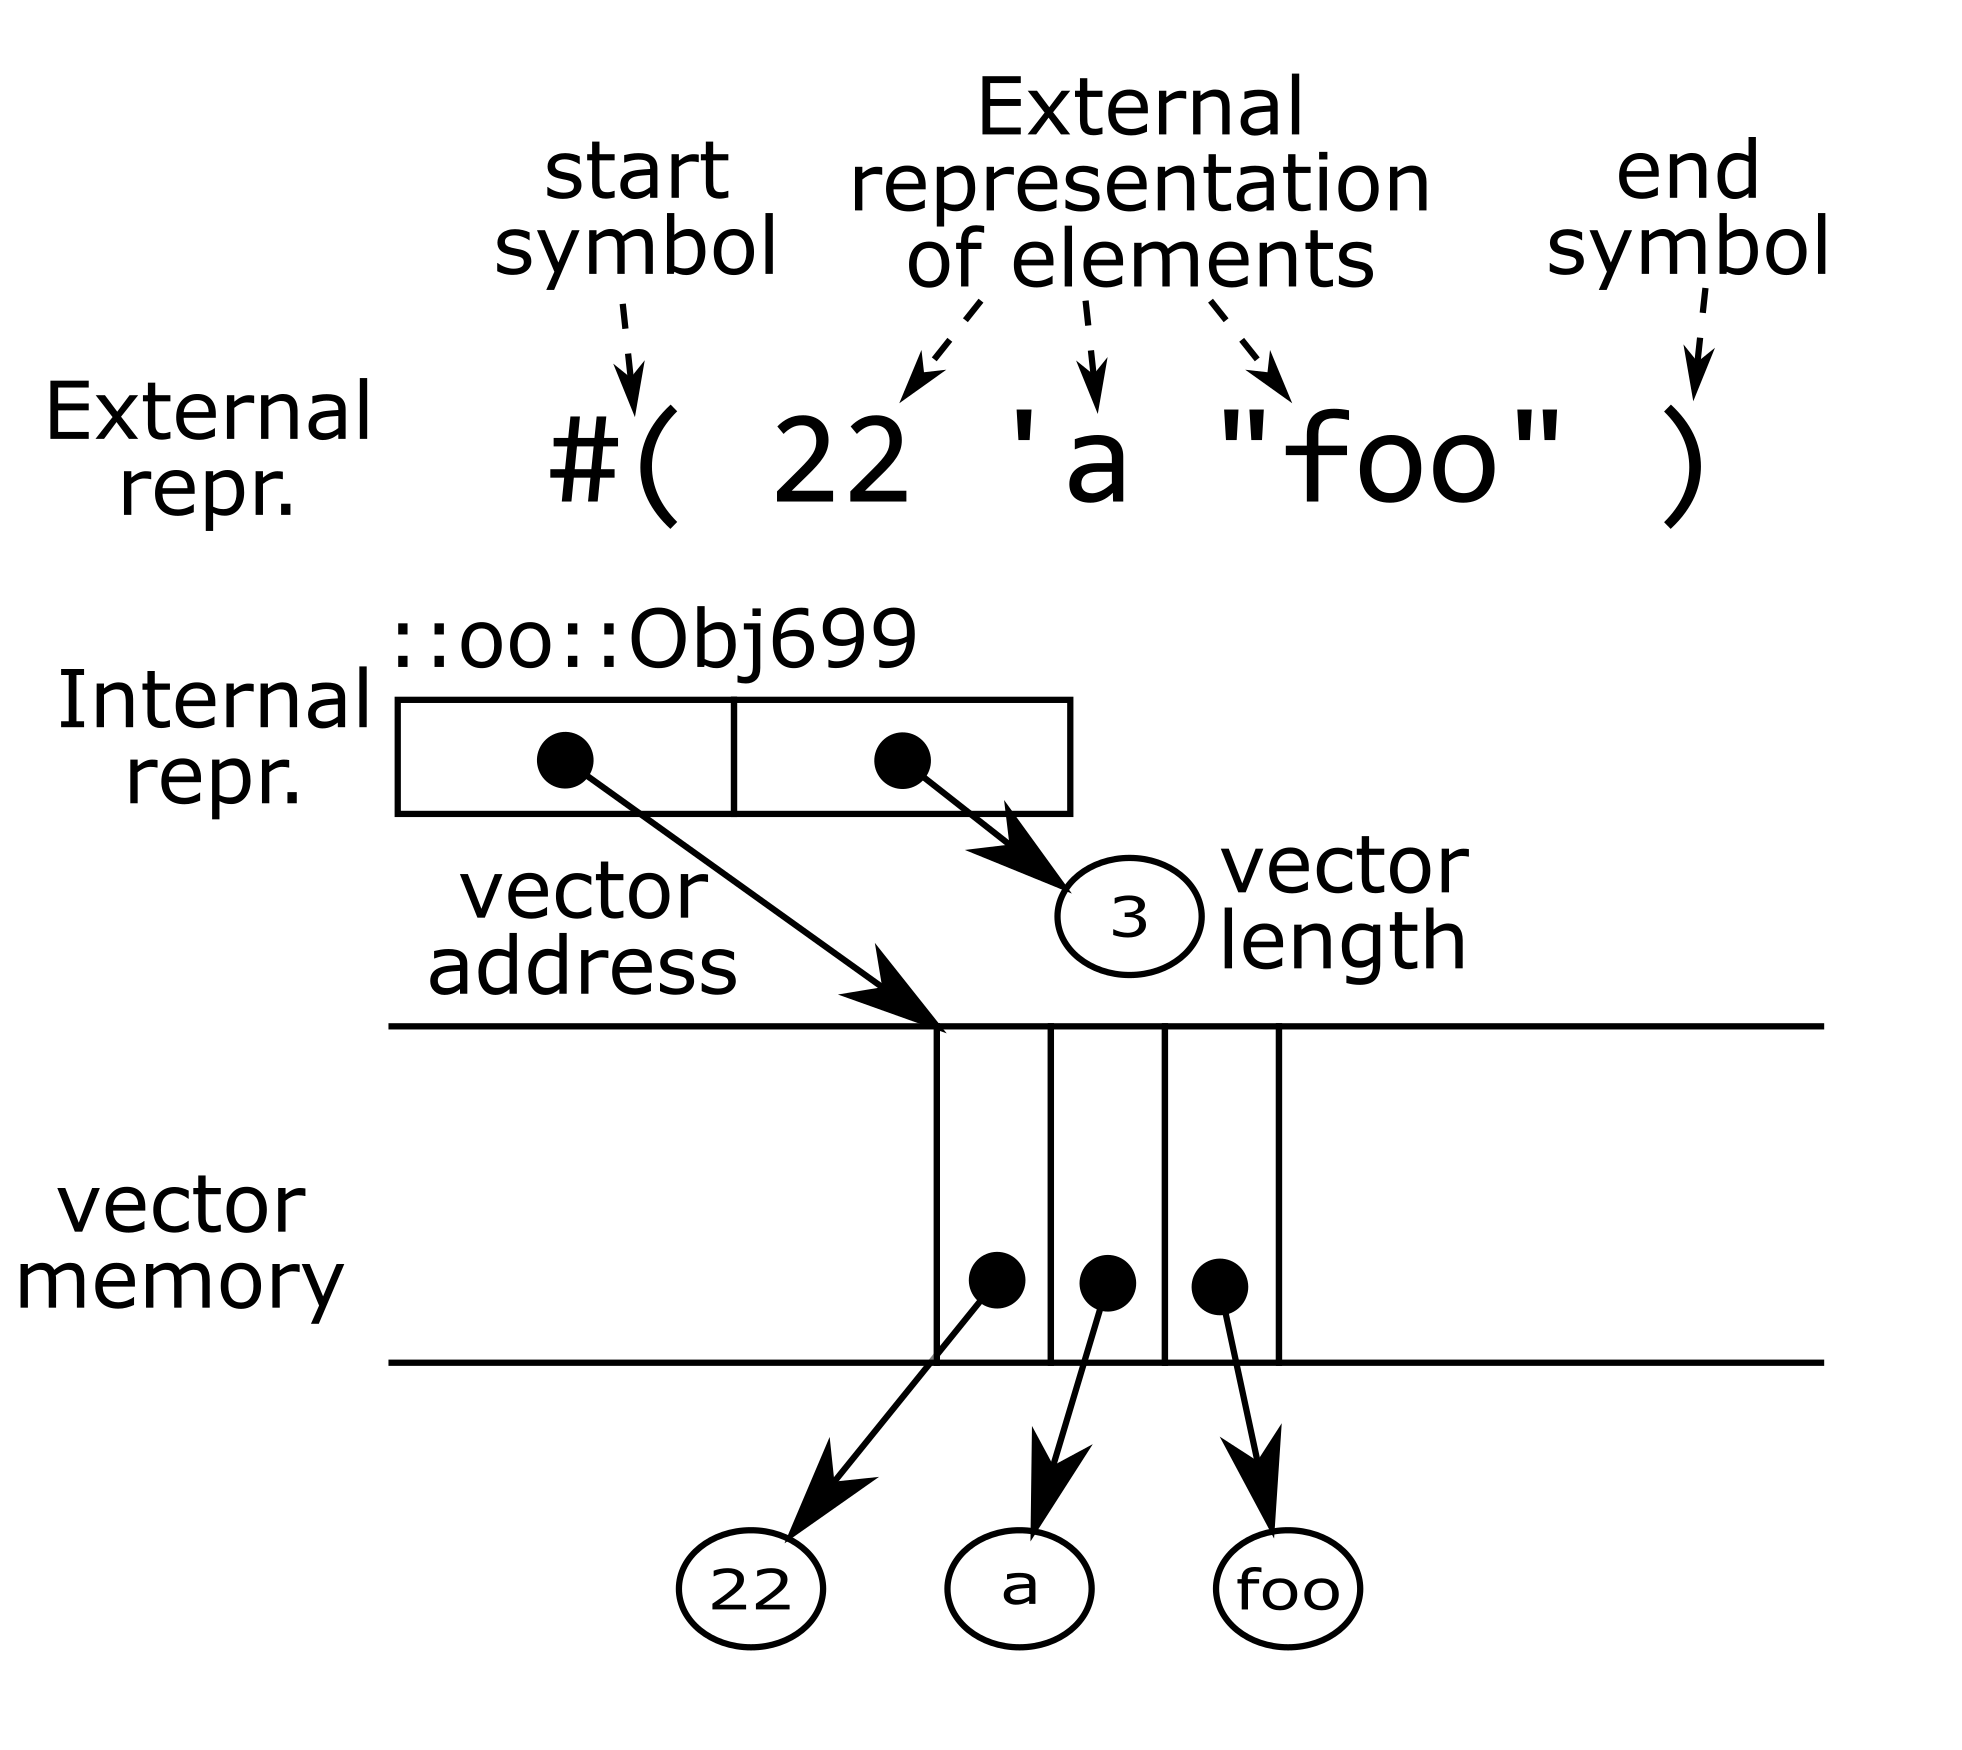
\includegraphics{images/vector-representation}


The \texttt{parse} procedure takes in the input buffer character by character, matching each character against a fitting external representation. When done, it creates a ConsTcl object, which is the internal representation of an expression. The object can then be passed to the evaluator.


Given a string, \texttt{parse} fills the input buffer. It then parses the input and produces the internal representation of an expression.


Example:

\noindent\makebox[\linewidth]{\rule{\linewidth}{0.4pt}}
\begin{lstlisting}
% ::constcl::parse "(+ 2 3)"
::oo::Obj491
\end{lstlisting}
\noindent\makebox[\linewidth]{\rule{\linewidth}{0.4pt}}

Here, \texttt{parse} parsed the external representation of a list with three elements, +, 2, and 3. It produced the expression that has an internal representation labeled \texttt{::oo::Obj491}. We will later meet procedures like \texttt{eval}, which transforms an expression into a value, and \texttt{write}, which prints a printed representation of expressions and values. Putting them together: we can see

\noindent\makebox[\linewidth]{\rule{\linewidth}{0.4pt}}
\begin{lstlisting}
% ::constcl::write ::oo::Obj491
(+ 2 3)
% ::constcl::eval ::oo::Obj491
::oo::Obj494
% ::constcl::write ::oo::Obj494
5
\end{lstlisting}
\noindent\makebox[\linewidth]{\rule{\linewidth}{0.4pt}}

Fortunately, we don't have to work at such a low level. We can use the \texttt{repl} instead:

\noindent\makebox[\linewidth]{\rule{\linewidth}{0.4pt}}
\begin{lstlisting}
ConsTcl> (+ 2 3)
5
\end{lstlisting}
\noindent\makebox[\linewidth]{\rule{\linewidth}{0.4pt}}

Then, parsing and evaluation and writing goes on in the background and the internal representations of expressions and values are hidden.


Anyway, here is how it really looks like. \texttt{::oo::Obj491} was just the head of the list.


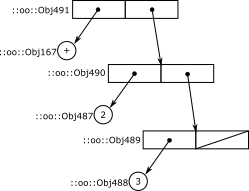
\includegraphics{images/intreplist.png}

\subsection{The parsing library}
\label{the-parsing-library}

\textbf{parse}


\texttt{parse} is the entry point into the \texttt{parse-} set of commands. It can be called with either a Tcl or ConsTcl string, or an input buffer (instance of IB). Once the input buffer is established, \texttt{parse} leaves control to \texttt{parse-expr}.

\begin{tabular}{ |l l| }
\hline
\multicolumn{2}{|l|}{parse (internal)} \\
\hline
inp & a Tcl string or an input buffer \\
\textit{Returns:} & an expression \\
\hline
\end{tabular}

\noindent\makebox[\linewidth]{\rule{\linewidth}{0.4pt}}
\begin{lstlisting}
reg parse
 
proc ::constcl::parse {inp} {
  if {[info object isa object $inp]} {
    if {[typeof? $inp IB] ne "#f"} {
      set ib $inp
    } elseif {[typeof? $inp String] ne "#f"} {
      set ib [IB new [$inp value]]
    } else {
      ::error "Unknown object [$inp show]"
    }
  } else {
    # It's a Tcl string, we hope
    set ib [IB new $inp]
  }
  return [parse-expr]
}
\end{lstlisting}
\noindent\makebox[\linewidth]{\rule{\linewidth}{0.4pt}}

\textbf{parse-expr}


The procedure \texttt{parse-expr} parses input by peeking at the first available character and delegating to one of the more detailed parsing procedures based on that, producing an expression of any kind.

\begin{tabular}{ |l l| }
\hline
\multicolumn{2}{|l|}{parse-expr (internal)} \\
\hline
\textit{Returns:} & an expression \\
\hline
\end{tabular}

\noindent\makebox[\linewidth]{\rule{\linewidth}{0.4pt}}
\begin{lstlisting}
proc ::constcl::parse-expr {} {
  upvar ib ib
  $ib skip-ws
  switch -regexp [$ib peek] {
    {\"}          { parse-string-expr }
    {\#}          { parse-sharp }
    {\'}          { parse-quoted-expr }
    {\(}          { parse-pair-expr ")" }
    {\+} - {\-}   { parse-plus-minus }
    {\,}          { parse-unquoted-expr }
    {\.} { $ib advance ; return [Dot new] }
    {\:}          { parse-object-expr }
    {\[}          { parse-pair-expr "\]" }
    {\`}          { parse-quasiquoted-expr }
    {\d}          { parse-number-expr }
    {^$}          { return}
    {[[:graph:]]} { parse-identifier-expr }
    default {
      ::error "unexpected character ([$ib peek])"
    }
  }
}
\end{lstlisting}
\noindent\makebox[\linewidth]{\rule{\linewidth}{0.4pt}}

\textbf{parse-string-expr}


\texttt{parse-string-expr} parses input starting with a double quote and collects characters until it reaches another (unescaped) double quote. It then returns a string expression--an immutable String (see page \pageref{strings}) object.

\begin{tabular}{ |l l| }
\hline
\multicolumn{2}{|l|}{parse-string-expr (internal)} \\
\hline
\textit{Returns:} & a string \\
\hline
\end{tabular}

\noindent\makebox[\linewidth]{\rule{\linewidth}{0.4pt}}
\begin{lstlisting}
proc ::constcl::parse-string-expr {} {
  upvar ib ib
  set str {}
  $ib advance
  while {[$ib peek] ne "\"" && [$ib peek] ne {}} {
    set c [$ib peek]
    if {$c eq "\\"} {
      ::append str $c
      $ib advance
      ::append str [$ib peek]
    } else {
      ::append str $c
    }
    $ib advance
  }
  if {[$ib peek] ne "\""} {
    ::error "no ending double quote"
  }
  $ib advance
  $ib skip-ws
  set expr [MkString $str]
  $expr mkconstant
  return $expr
}
\end{lstlisting}
\noindent\makebox[\linewidth]{\rule{\linewidth}{0.4pt}}

\textbf{parse-sharp}


\texttt{parse-sharp} parses input starting with a sharp sign (\#) and either produces the boolean literals, or delegates to the vector parser (if the next character is a left parenthesis) or the character parser (if it is a backslash).

\begin{tabular}{ |l l| }
\hline
\multicolumn{2}{|l|}{parse-sharp (internal)} \\
\hline
\textit{Returns:} & a vector, boolean, or character value \\
\hline
\end{tabular}

\noindent\makebox[\linewidth]{\rule{\linewidth}{0.4pt}}
\begin{lstlisting}
proc ::constcl::parse-sharp {} {
  upvar ib ib
  $ib advance
  switch [$ib peek] {
    "("  { return [parse-vector-expr] }
    "t"  { $ib advance ; $ib skip-ws ; return #t }
    "f"  { $ib advance ; $ib skip-ws ; return #f }
    "\\" { return [parse-character-expr] }
    default {
      ::error "Illegal #-literal: #[$ib peek]"
    }
  }
}
\end{lstlisting}
\noindent\makebox[\linewidth]{\rule{\linewidth}{0.4pt}}

\textbf{make-constant}


The \texttt{make-constant} helper procedure is called to set components of expressions to constants when read as a quoted literal.

\noindent\makebox[\linewidth]{\rule{\linewidth}{0.4pt}}
\begin{lstlisting}
proc ::constcl::make-constant {val} {
  if {[pair? $val] ne "#f"} {
    $val mkconstant
    make-constant [car $val]
    make-constant [cdr $val]
  } elseif {[null? $val] ne "#f"} {
    return #NIL
  } else {
    $val mkconstant
  }
}
\end{lstlisting}
\noindent\makebox[\linewidth]{\rule{\linewidth}{0.4pt}}

\textbf{parse-quoted-expr}


\texttt{parse-quoted-expr} parses input starting with an apostrophe ("'"), and then parses an entire expression beyond that, returning it wrapped in a list with \texttt{quote}. The quoted expression is made constant.

\begin{tabular}{ |l l| }
\hline
\multicolumn{2}{|l|}{parse-quoted-expr (internal)} \\
\hline
\textit{Returns:} & an expression wrapped in the quote symbol \\
\hline
\end{tabular}

\noindent\makebox[\linewidth]{\rule{\linewidth}{0.4pt}}
\begin{lstlisting}
proc ::constcl::parse-quoted-expr {} {
  upvar ib ib
  $ib advance
  set expr [parse-expr]
  $ib skip-ws
  make-constant $expr
  return [list [S quote] $expr]
}
\end{lstlisting}
\noindent\makebox[\linewidth]{\rule{\linewidth}{0.4pt}}

\textbf{parse-pair-expr}


The \texttt{parse-pair-expr} procedure parses everything between two matching parentheses, or, as the case might be, brackets. It produces a possibly recursive structure of Pair (see page \pageref{pairs-and-lists) objects, either a proper list (one that ends in \#NIL) or an improper one (one that has an atom as its last member}), or in some cases an empty list.

\begin{tabular}{ |l l| }
\hline
\multicolumn{2}{|l|}{parse-pair-expr (internal)} \\
\hline
char & the terminating paren or bracket \\
\textit{Returns:} & a structure of pair expressions \\
\hline
\end{tabular}

\noindent\makebox[\linewidth]{\rule{\linewidth}{0.4pt}}
\begin{lstlisting}
proc ::constcl::parse-pair-expr {char} {
  upvar ib ib
  $ib advance
  $ib skip-ws
  set expr [parse-pair $char]
  $ib skip-ws
  if {[$ib peek] ne $char} {
    if {$char eq ")"} {
      ::error \
        "Missing right paren. ([$ib peek])."
    } else {
      ::error \
        "Missing right bracket ([$ib peek])."
    }
  }
  $ib advance
  $ib skip-ws
  return $expr
}
\end{lstlisting}
\noindent\makebox[\linewidth]{\rule{\linewidth}{0.4pt}}

\texttt{parse-pair} is a helper procedure that does the heavy lifting in parsing a pair structure. First it checks if the list is empty, returning \#NIL in that case. Then it parses the first element in the list and then repeatedly the rest of them. If it parses a Dot object, the following element to be read is the tail of an improper list. When \texttt{parse-pair} has reached the ending parenthesis or bracket, it conses up the elements starting from the last, and returns the head of the list.

\noindent\makebox[\linewidth]{\rule{\linewidth}{0.4pt}}
\begin{lstlisting}
proc ::constcl::parse-pair {char} {
  upvar ib ib
  if {[$ib find $char]} {
    return #NIL
  }
  $ib skip-ws
  set a [parse-expr]
  $ib skip-ws
  set res $a
  set prev #NIL
  while {![$ib find $char]} {
    set x [parse-expr]
    $ib skip-ws
    if {[dot? $x] ne "#f"} {
      set prev [parse-expr]
      $ib skip-ws
    } else {
      lappend res $x
    }
    if {[llength $res] > 999} break
  }
  foreach r [lreverse $res] {
    set prev [cons $r $prev]
  }
  return $prev
}
\end{lstlisting}
\noindent\makebox[\linewidth]{\rule{\linewidth}{0.4pt}}

\textbf{parse-plus-minus}


\texttt{parse-plus-minus} reacts to a plus or minus in the input buffer, and either returns a \texttt{+} or \texttt{-} symbol, or a number.

\begin{tabular}{ |l l| }
\hline
\multicolumn{2}{|l|}{parse-plus-minus (internal)} \\
\hline
\textit{Returns:} & either the symbols + or - or a number \\
\hline
\end{tabular}

\noindent\makebox[\linewidth]{\rule{\linewidth}{0.4pt}}
\begin{lstlisting}
proc ::constcl::parse-plus-minus {} {
  upvar ib ib
  set c [$ib peek]
  $ib advance
  if {[::string is digit -strict [$ib peek]]} {
    $ib unget $c
    return [::constcl::parse-number-expr]
  } else {
    if {$c eq "+"} {
      $ib skip-ws
      return [MkSymbol "+"]
    } else {
      $ib skip-ws
      return [MkSymbol "-"]
    }
  }
}
\end{lstlisting}
\noindent\makebox[\linewidth]{\rule{\linewidth}{0.4pt}}

\textbf{parse-unquoted-expr}


\texttt{parse-unquoted-expr} parses input, producing an expression and returning it wrapped in \texttt{unquote}, or in \texttt{unquote-splicing} if an @-sign is present in the input stream.

\begin{tabular}{ |l l| }
\hline
\multicolumn{2}{|l|}{parse-unquoted-expr (internal)} \\
\hline
\textit{Returns:} & an expression wrapped in the unquote/-splicing symbol \\
\hline
\end{tabular}

\noindent\makebox[\linewidth]{\rule{\linewidth}{0.4pt}}
\begin{lstlisting}
proc ::constcl::parse-unquoted-expr {} {
  upvar ib ib
  $ib advance
  set symbol "unquote"
  if {[$ib peek] eq "@"} {
    set symbol "unquote-splicing"
    $ib advance
  }
  set expr [parse-expr]
  $ib skip-ws
  return [list [MkSymbol $symbol] $expr]
}
\end{lstlisting}
\noindent\makebox[\linewidth]{\rule{\linewidth}{0.4pt}}

\textbf{parse-quasiquoted-expr}


\texttt{parse-quasiquoted-expr} parses input, producing an expression and returning it wrapped in \texttt{quasiquote}.

\begin{tabular}{ |l l| }
\hline
\multicolumn{2}{|l|}{parse-quasiquoted-expr (internal)} \\
\hline
\textit{Returns:} & an expression wrapped in the quasiquote symbol \\
\hline
\end{tabular}

\noindent\makebox[\linewidth]{\rule{\linewidth}{0.4pt}}
\begin{lstlisting}
proc ::constcl::parse-quasiquoted-expr {} {
  upvar ib ib
  $ib advance
  set expr [parse-expr]
  $ib skip-ws
  make-constant $expr
  return [list [MkSymbol "quasiquote"] $expr]
}
\end{lstlisting}
\noindent\makebox[\linewidth]{\rule{\linewidth}{0.4pt}}

\textbf{interspace}


The \texttt{interspace} helper procedure recognizes whitespace between value representations.

\noindent\makebox[\linewidth]{\rule{\linewidth}{0.4pt}}
\begin{lstlisting}
proc ::constcl::interspace {c} {
  # don't add #EOF: parse-* uses this one too
  if {$c eq {} ||
    [::string is space $c] ||
    $c eq ";"} {
      return #t
    } else {
      return #f
    }
}
\end{lstlisting}
\noindent\makebox[\linewidth]{\rule{\linewidth}{0.4pt}}

\textbf{parse-number-expr}


\texttt{parse-number-expr} parses input, producing a number and returning a Number (see page \pageref{numbers}) object.

\begin{tabular}{ |l l| }
\hline
\multicolumn{2}{|l|}{parse-number-expr (internal)} \\
\hline
\textit{Returns:} & a number \\
\hline
\end{tabular}

\noindent\makebox[\linewidth]{\rule{\linewidth}{0.4pt}}
\begin{lstlisting}
proc ::constcl::parse-number-expr {} {
  upvar ib ib
  while {[interspace [$ib peek]] ne "#t" && \
    [$ib peek] ni {) \]}} {
      ::append num [$ib peek]
      $ib advance
    }
    $ib skip-ws
    check {::string is double -strict $num} {
      Invalid numeric constant $num
    }
    return [MkNumber $num]
}
\end{lstlisting}
\noindent\makebox[\linewidth]{\rule{\linewidth}{0.4pt}}

\textbf{parse-identifier-expr}


\texttt{parse-identifier-expr} parses input, producing an identifier expression and returning a Symbol (see page \pageref{symbols}) object.

\begin{tabular}{ |l l| }
\hline
\multicolumn{2}{|l|}{parse-identifier-expr (internal)} \\
\hline
\textit{Returns:} & a symbol \\
\hline
\end{tabular}

\noindent\makebox[\linewidth]{\rule{\linewidth}{0.4pt}}
\begin{lstlisting}
proc ::constcl::parse-identifier-expr {} {
  upvar ib ib
  while {[interspace [$ib peek]] ne "#t" &&
      [$ib peek] ni {) \]}} {
    ::append name [$ib peek]
    $ib advance
  }
  $ib skip-ws
  # idcheck throws error if invalid identifier
  return [MkSymbol [idcheck $name]]
}
\end{lstlisting}
\noindent\makebox[\linewidth]{\rule{\linewidth}{0.4pt}}

\textbf{character-check}


The \texttt{character-check} helper procedure compares a potential character constant to the valid kinds.

\begin{tabular}{ |l l| }
\hline
\multicolumn{2}{|l|}{character-check (internal)} \\
\hline
name & a Tcl string \\
\textit{Returns:} & a Tcl truth value (1 or 0) \\
\hline
\end{tabular}

\noindent\makebox[\linewidth]{\rule{\linewidth}{0.4pt}}
\begin{lstlisting}
proc ::constcl::character-check {name} {
  if {[regexp {(?i)^#\\([[:graph:]]|space|newline)$} \
      $name]} {
    return #t
  } else {
    return #f
  }
}
\end{lstlisting}
\noindent\makebox[\linewidth]{\rule{\linewidth}{0.4pt}}

\textbf{parse-character-expr}


\texttt{parse-character-expr} parses input, producing a character and returning a Char (see page \pageref{characters}) object.

\begin{tabular}{ |l l| }
\hline
\multicolumn{2}{|l|}{parse-character-expr (internal)} \\
\hline
\textit{Returns:} & a character \\
\hline
\end{tabular}

\noindent\makebox[\linewidth]{\rule{\linewidth}{0.4pt}}
\begin{lstlisting}
proc ::constcl::parse-character-expr {} {
  upvar ib ib
  set name "#"
  while {[interspace [$ib peek]] ne "#t" &&
      [$ib peek] ni {) ]}} {
    ::append name [$ib peek]
    $ib advance
  }
  check {character-check $name} {
    Invalid character constant $name
  }
  $ib skip-ws
  return [MkChar $name]
}
\end{lstlisting}
\noindent\makebox[\linewidth]{\rule{\linewidth}{0.4pt}}

\textbf{parse-vector-expr}


\texttt{parse-vector-expr} parses input, producing a vector expression and returning a Vector (see page \pageref{vectors}) object.

\begin{tabular}{ |l l| }
\hline
\multicolumn{2}{|l|}{parse-vector-expr (internal)} \\
\hline
\textit{Returns:} & a vector \\
\hline
\end{tabular}

\noindent\makebox[\linewidth]{\rule{\linewidth}{0.4pt}}
\begin{lstlisting}
proc ::constcl::parse-vector-expr {} {
  upvar ib ib
  $ib advance
  $ib skip-ws
  set res {}
  while {[$ib peek] ne {} && [$ib peek] ne ")"} {
    lappend res [parse-expr]
    $ib skip-ws
  }
  set vec [MkVector $res]
  $vec mkconstant
  if {[$ib peek] ne ")"} {
    ::error "Missing right parenthesis."
  }
  $ib advance
  $ib skip-ws
  return $vec
}
\end{lstlisting}
\noindent\makebox[\linewidth]{\rule{\linewidth}{0.4pt}}

\textbf{parse-object-expr}


A non-standard extension, \texttt{parse-object-expr} reads one of the ConsTcl objects and passes its name along.

\begin{tabular}{ |l l| }
\hline
\multicolumn{2}{|l|}{parse-object-expr (internal)} \\
\hline
\textit{Returns:} & a ConsTcl object \\
\hline
\end{tabular}

\noindent\makebox[\linewidth]{\rule{\linewidth}{0.4pt}}
\begin{lstlisting}
proc ::constcl::parse-object-expr {} {
  upvar ib ib
  foreach ch [split "::oo::Obj" {}] {
    if {[$ib peek] ne $ch} {
      error "bad object name"
    }
    $ib advance
  }
  set res "::oo::Obj"
  while {[::string is digit [$ib peek]]} {
    ::append res [$ib peek]
    $ib advance
  }
  return $res
}
\end{lstlisting}
\noindent\makebox[\linewidth]{\rule{\linewidth}{0.4pt}}
\section{read}
\label{read}

\textbf{read}


The standard builtin \texttt{read} reads and parses input into a Lisp expression in a similar manner to how \texttt{parse} parses a string buffer.

\begin{tabular}{ |l l| }
\hline
\multicolumn{2}{|l|}{read (public)} \\
\hline
?port? & a port \\
\textit{Returns:} & an expression \\
\hline
\end{tabular}

\noindent\makebox[\linewidth]{\rule{\linewidth}{0.4pt}}
\begin{lstlisting}
reg read
 
proc ::constcl::read {args} {
  set c {}
  set unget {}
  if {[llength $args]} {
    lassign $args port
  } else {
    set port $::constcl::Input_port
  }
  set oldport $::constcl::Input_port
  set ::constcl::Input_port $port
  set expr [read-expr]
  set ::constcl::Input_port $oldport
  return $expr
}
\end{lstlisting}
\noindent\makebox[\linewidth]{\rule{\linewidth}{0.4pt}}

\textbf{read-expr}


The procedure \texttt{read-expr} parses input by reading the first available character and delegating to one of the more detailed reading procedures based on that, producing an expression of any kind. A Tcl character value can be passed to it, that character will be used first before reading from the input stream. If the end of file is encountered before an expression can be read in full, the procedure returns end of file.

\begin{tabular}{ |l l| }
\hline
\multicolumn{2}{|l|}{read-expr (internal)} \\
\hline
?char? & a Tcl character \\
\textit{Returns:} & an expression or end of file \\
\hline
\end{tabular}

\noindent\makebox[\linewidth]{\rule{\linewidth}{0.4pt}}
\begin{lstlisting}
proc ::constcl::read-expr {args} {
  upvar c c unget unget
  if {[llength $args]} {
    lassign $args c
  } else {
    set c [readc]
  }
  read-eof $c
  if {[::string is space $c] || $c eq ";"} {
    skip-ws
    read-eof $c
  }
  switch -regexp $c {
    {\"}          { read-string-expr }
    {\#}          { read-sharp }
    {\'}          { read-quoted-expr }
    {\(}          { read-pair-expr ")" }
    {\+} - {\-}   { read-plus-minus $c }
    {\,}          { read-unquoted-expr }
    {\.}          { Dot new }
    {\:}          { read-object-expr }
    {\[}          { read-pair-expr "\]" }
    {\`}          { read-quasiquoted-expr }
    {\d}          { read-number-expr $c }
    {^$}          { return}
    {[[:graph:]]} { read-identifier-expr $c }
    default {
      read-eof $c
      ::error "unexpected character ($c)"
    }
  }
}
\end{lstlisting}
\noindent\makebox[\linewidth]{\rule{\linewidth}{0.4pt}}

\texttt{readc} reads one character either from the unget store or from the input stream. If the input stream is at end-of-file, an eof object is returned.

\begin{tabular}{ |l l| }
\hline
\multicolumn{2}{|l|}{readc (internal)} \\
\hline
\textit{Returns:} & a Tcl character or end of file \\
\hline
\end{tabular}

\noindent\makebox[\linewidth]{\rule{\linewidth}{0.4pt}}
\begin{lstlisting}
proc readc {} {
  upvar unget unget
  if {$unget ne {}} {
    set c $unget
    set unget {}
  } else {
    set c [::read [$::constcl::Input_port handle] 1]
    if {[eof [$::constcl::Input_port handle]]} {
      return #EOF
    }
  }
  return $c
}
\end{lstlisting}
\noindent\makebox[\linewidth]{\rule{\linewidth}{0.4pt}}

\texttt{read-find} reads ahead through whitespace to find a given character. Returns 1 if it has found the character, and 0 if it has stopped at some other character. Returns end of file if eof is encountered.

\begin{tabular}{ |l l| }
\hline
\multicolumn{2}{|l|}{read-find (internal)} \\
\hline
char & a Tcl character \\
\textit{Returns:} & a Tcl truth value (1 or 0) or end of file \\
\hline
\end{tabular}

\noindent\makebox[\linewidth]{\rule{\linewidth}{0.4pt}}
\begin{lstlisting}
proc read-find {char} {
  upvar c c unget unget
  while {[::string is space -strict $c]} {
    set c [readc]
    read-eof $c
    set unget $c
  }
  return [expr {$c eq $char}]
}
\end{lstlisting}
\noindent\makebox[\linewidth]{\rule{\linewidth}{0.4pt}}

\texttt{skip-ws} skips whitespace and comments (the ; to end of line kind). Uses the shared \_c\_ character. It leaves the first character not to be skipped in \_c\_.

\begin{tabular}{ |l l| }
\hline
\multicolumn{2}{|l|}{skip-ws (internal)} \\
\hline
\textit{Returns:} & nothing \\
\hline
\end{tabular}

\noindent\makebox[\linewidth]{\rule{\linewidth}{0.4pt}}
\begin{lstlisting}
proc skip-ws {} {
  upvar c c unget unget
  while true {
    switch -regexp $c {
      {[[:space:]]} {
        set c [readc]
      }
      {;} {
        while {$c ne "\n" && $c ne "#EOF"}  {
          set c [readc]
        }
      }
      default {
        return
      }
    }
  }
}
\end{lstlisting}
\noindent\makebox[\linewidth]{\rule{\linewidth}{0.4pt}}

\texttt{read-eof} checks a number of characters for possible end-of-file objects. If it finds one, it returns \emph{from its caller} with the EOF value.

\begin{tabular}{ |l l| }
\hline
\multicolumn{2}{|l|}{read-eof (internal)} \\
\hline
args & some characters \\
\hline
\end{tabular}

\noindent\makebox[\linewidth]{\rule{\linewidth}{0.4pt}}
\begin{lstlisting}
proc read-eof {args} {
  foreach val $args {
    if {$val eq "#EOF"} {
      return -level 1 -code return #EOF
    }
  }
}
\end{lstlisting}
\noindent\makebox[\linewidth]{\rule{\linewidth}{0.4pt}}

\textbf{read-string-expr}


\texttt{read-string-expr} parses input starting with a double quote and collects characters until it reaches another (unescaped) double quote. It then returns a string expression--an immutable String (see page \pageref{strings}) object.

\begin{tabular}{ |l l| }
\hline
\multicolumn{2}{|l|}{read-string-expr (internal)} \\
\hline
\textit{Returns:} & a string or end of file \\
\hline
\end{tabular}

\noindent\makebox[\linewidth]{\rule{\linewidth}{0.4pt}}
\begin{lstlisting}
proc ::constcl::read-string-expr {} {
  upvar c c unget unget
  set str {}
  set c [readc]
  read-eof $c
  while {$c ne "\"" && $c ne "#EOF"} {
    if {$c eq "\\"} {
      ::append str $v
      set c [readc]
    }
    ::append str $c
    set c [readc]
  }
  if {$c ne "\""} {
    error "bad string (no ending double quote)"
  }
  set c [readc]
  set expr [MkString $str]
  read-eof $expr
  $expr mkconstant
  return $expr
}
\end{lstlisting}
\noindent\makebox[\linewidth]{\rule{\linewidth}{0.4pt}}

\textbf{read-sharp}


\texttt{read-sharp} parses input starting with a sharp sign (\#) and produces the various kinds of expressions whose external representation begins with a sharp sign.

\begin{tabular}{ |l l| }
\hline
\multicolumn{2}{|l|}{read-sharp (internal)} \\
\hline
\textit{Returns:} & a vector, boolean, or character value or end of file \\
\hline
\end{tabular}

\noindent\makebox[\linewidth]{\rule{\linewidth}{0.4pt}}
\begin{lstlisting}
proc ::constcl::read-sharp {} {
  upvar c c unget unget
  set c [readc]
  read-eof $c
  switch $c {
    (    { set n [read-vector-expr] }
    t    { set n #t }
    f    { set n #f }
    "\\" { set n [read-character-expr] }
    default {
      read-eof $c
      ::error "Illegal #-literal: #$c"
    }
  }
  set c [readc]
  return $n
}
\end{lstlisting}
\noindent\makebox[\linewidth]{\rule{\linewidth}{0.4pt}}

\textbf{read-vector-expr}


\texttt{read-vector-expr} parses input, producing a vector expression and returning a Vector (see page \pageref{vectors}) object.

\begin{tabular}{ |l l| }
\hline
\multicolumn{2}{|l|}{read-vector-expr (internal)} \\
\hline
\textit{Returns:} & a vector or end of file \\
\hline
\end{tabular}

\noindent\makebox[\linewidth]{\rule{\linewidth}{0.4pt}}
\begin{lstlisting}
proc ::constcl::read-vector-expr {} {
  upvar c c unget unget
  set res {}
  set c [readc]
  while {$c ne "#EOF" && $c ne ")"} {
    lappend res [read-expr $c]
    skip-ws
    read-eof $c
  }
  set expr [MkVector $res]
  read-eof $expr
  $expr mkconstant
  if {$c ne ")"} {
    ::error "Missing right paren. ($c)."
  }
  set c [readc]
  return $expr
}
\end{lstlisting}
\noindent\makebox[\linewidth]{\rule{\linewidth}{0.4pt}}

\textbf{read-character-expr}


\texttt{read-character-expr} parses input, producing a character and returning a Char (see page \pageref{characters}) object.

\begin{tabular}{ |l l| }
\hline
\multicolumn{2}{|l|}{read-character-expr (internal)} \\
\hline
\textit{Returns:} & a character or end of file \\
\hline
\end{tabular}

\noindent\makebox[\linewidth]{\rule{\linewidth}{0.4pt}}
\begin{lstlisting}
proc ::constcl::read-character-expr {} {
  upvar c c unget unget
  set name "#\\"
  set c [readc]
  read-eof $c
  while {[::string is alpha $c]} {
    ::append name $c
    set c [readc]
    read-eof $c
  }
  check {character-check $name} {
      Invalid character constant $name
  }
  set expr [MkChar $name]
  read-eof $expr
  return $expr
}
\end{lstlisting}
\noindent\makebox[\linewidth]{\rule{\linewidth}{0.4pt}}

\textbf{read-quoted-expr}


\texttt{read-quoted-expr} parses input starting with a "'", and then parses an entire expression beyond that, returning it wrapped in a list with \texttt{quote}.

\begin{tabular}{ |l l| }
\hline
\multicolumn{2}{|l|}{read-quoted-expr (internal)} \\
\hline
\textit{Returns:} & an expression wrapped in the quote symbol or end of file \\
\hline
\end{tabular}

\noindent\makebox[\linewidth]{\rule{\linewidth}{0.4pt}}
\begin{lstlisting}
proc ::constcl::read-quoted-expr {} {
  upvar c c unget unget
  set expr [read-expr]
  read-eof $expr
  make-constant $expr
  return [list [S quote] $expr]
}
\end{lstlisting}
\noindent\makebox[\linewidth]{\rule{\linewidth}{0.4pt}}

\textbf{read-pair-expr}


The \texttt{read-pair-expr} procedure parses input and produces a structure of Pair (see page \pageref{pairs-and-lists})s expression.

\begin{tabular}{ |l l| }
\hline
\multicolumn{2}{|l|}{read-pair-expr (internal)} \\
\hline
char & the terminating paren or bracket \\
\textit{Returns:} & a structure of pair expressions or end of file \\
\hline
\end{tabular}

\noindent\makebox[\linewidth]{\rule{\linewidth}{0.4pt}}
\begin{lstlisting}
proc ::constcl::read-pair-expr {char} {
  upvar c c unget unget
  set expr [read-pair $char]
  read-eof $expr
  skip-ws
  read-eof $c
  if {$c ne $char} {
    if {$char eq ")"} {
      ::error \
        "Missing right paren. ($c)."
    } else {
      ::error \
        "Missing right bracket ($c)."
    }
  } else {
    set unget {}
    set c [readc]
  }
  return $expr
}
 
proc ::constcl::read-pair {char} {
  upvar c c unget unget
  if {[read-find $char]} {
    # read right paren/brack
    set c [readc]
    return #NIL
  }
  set c [readc]
  read-eof $c
  set a [read-expr $c]
  set res $a
  skip-ws
  set prev #NIL
  while {![read-find $char]} {
    set x [read-expr $c]
    skip-ws
    read-eof $c
    if {[dot? $x] ne "#f"} {
      set prev [read-expr $c]
      skip-ws $c]
      read-eof $c
    } else {
      lappend res $x
    }
    if {[llength $res] > 999} break
  }
  # read right paren/brack
  foreach r [lreverse $res] {
    set prev [cons $r $prev]
  }
  return $prev
}
\end{lstlisting}
\noindent\makebox[\linewidth]{\rule{\linewidth}{0.4pt}}

\textbf{read-plus-minus}


\texttt{read-plus-minus} reacts to a plus or minus in the input stream, and either returns a \texttt{+} or \texttt{-} symbol, or a number.

\begin{tabular}{ |l l| }
\hline
\multicolumn{2}{|l|}{read-plus-minus (internal)} \\
\hline
\textit{Returns:} & either the symbols + or - or a number or end of file \\
\hline
\end{tabular}

\noindent\makebox[\linewidth]{\rule{\linewidth}{0.4pt}}
\begin{lstlisting}
proc ::constcl::read-plus-minus {char} {
  upvar c c unget unget
  set c [readc]
  read-eof $c
  if {[::string is digit -strict $c]} {
    set n [read-number-expr $c]
    if {$char eq "-"} {
      set n [- $n]
    }
    return $n
  } else {
    if {$char eq "+"} {
      return [MkSymbol "+"]
    } else {
      return [MkSymbol "-"]
    }
  }
}
\end{lstlisting}
\noindent\makebox[\linewidth]{\rule{\linewidth}{0.4pt}}

\textbf{read-number-expr}


\texttt{read-number-expr} parses input, producing a number and returning a Number (see page \pageref{numbers}) object.

\begin{tabular}{ |l l| }
\hline
\multicolumn{2}{|l|}{read-number-expr (internal)} \\
\hline
?char? & a Tcl character \\
\textit{Returns:} & a number or end of file \\
\hline
\end{tabular}

\noindent\makebox[\linewidth]{\rule{\linewidth}{0.4pt}}
\begin{lstlisting}
proc ::constcl::read-number-expr {args} {
  upvar c c unget unget
  if {[llength $args]} {
    lassign $args c
  } else {
    set c [readc]
  }
  read-eof $c
  while {[interspace $c] ne "#t" && $c ne "#EOF" &&
      $c ni {) \]}} {
    ::append num $c
    set c [readc]
  }
  set unget $c
  check {::string is double -strict $num} {
      Invalid numeric constant $num
  }
  set expr [MkNumber $num]
  read-eof $expr
  return $expr
}
\end{lstlisting}
\noindent\makebox[\linewidth]{\rule{\linewidth}{0.4pt}}

\textbf{read-unquoted-expr}


\texttt{read-unquoted-expr} parses input, producing an expression and returning it wrapped in \texttt{unquote}, or in \texttt{unquote-splicing} if an @-sign is present in the input stream.

\begin{tabular}{ |l l| }
\hline
\multicolumn{2}{|l|}{read-unquoted-expr (internal)} \\
\hline
\textit{Returns:} & an expr. wr. in the unquote/-splicing symbol or end of file \\
\hline
\end{tabular}

\noindent\makebox[\linewidth]{\rule{\linewidth}{0.4pt}}
\begin{lstlisting}
proc ::constcl::read-unquoted-expr {} {
  upvar c c unget unget
  set c [readc]
  read-eof $c
  if {$c eq "@"} {
    set symbol "unquote-splicing"
    set expr [read-expr]
  } else {
    set symbol "unquote"
    set expr [read-expr $c]
  }
  read-eof $expr
  return [list [MkSymbol $symbol] $expr]
}
\end{lstlisting}
\noindent\makebox[\linewidth]{\rule{\linewidth}{0.4pt}}

\textbf{read-object-expr}


A non-standard extension, \texttt{read-object-expr} reads one of the ConsTcl objects and passes its name along.

\begin{tabular}{ |l l| }
\hline
\multicolumn{2}{|l|}{read-object-expr (internal)} \\
\hline
\textit{Returns:} & a ConsTcl object or end of file \\
\hline
\end{tabular}

\noindent\makebox[\linewidth]{\rule{\linewidth}{0.4pt}}
\begin{lstlisting}
proc ::constcl::read-object-expr {} {
  upvar c c unget unget
  foreach ch [split ":oo::Obj" {}] {
    set c [readc]
    read-eof $c
    if {$c ne $ch} {
      error "bad object name"
    }
  }
  set res "::oo::Obj"
  set c [readc]
  read-eof $c
  while {[::string is digit $c]} {
    ::append res $c
    set c [readc]
    read-eof $c
  }
  set unget $c
  return $res
}
\end{lstlisting}
\noindent\makebox[\linewidth]{\rule{\linewidth}{0.4pt}}

\textbf{read-quasiquoted-expr}


\texttt{read-quasiquoted-expr} parses input, producing an expression and returning it wrapped in \texttt{quasiquote}.

\begin{tabular}{ |l l| }
\hline
\multicolumn{2}{|l|}{read-quasiquoted-expr (internal)} \\
\hline
\textit{Returns:} & an expr. wr. in the quasiquote symbol or end of file \\
\hline
\end{tabular}

\noindent\makebox[\linewidth]{\rule{\linewidth}{0.4pt}}
\begin{lstlisting}
proc ::constcl::read-quasiquoted-expr {} {
  upvar c c unget unget
  set expr [read-expr]
  skip-ws
  read-eof $expr
  make-constant $expr
  return [list [MkSymbol "quasiquote"] $expr]
}
\end{lstlisting}
\noindent\makebox[\linewidth]{\rule{\linewidth}{0.4pt}}

\textbf{read-identifier-expr}


\texttt{read-identifier-expr} parses input, producing an identifier expression and returning a Symbol (see page \pageref{symbols}) object.

\begin{tabular}{ |l l| }
\hline
\multicolumn{2}{|l|}{read-identifier-expr (internal)} \\
\hline
?char? & a Tcl character \\
\textit{Returns:} & a symbol or end of file \\
\hline
\end{tabular}

\noindent\makebox[\linewidth]{\rule{\linewidth}{0.4pt}}
\begin{lstlisting}
proc ::constcl::read-identifier-expr {args} {
  upvar c c unget unget
  if {[llength $args]} {
    lassign $args c
  } else {
    set c [readc]
  }
  read-eof $c
  set name {}
  while {[::string is graph -strict $c]} {
    if {$c eq "#EOF" || $c in {) \]}} {
      break
    }
    ::append name $c
    set c [readc]
  }
  if {$c ne "#EOF"} {
    set unget $c
  }
  read-eof $name
  # idcheck throws error if invalid identifier
  idcheck $name
  return [MkSymbol $name]
}
\end{lstlisting}
\noindent\makebox[\linewidth]{\rule{\linewidth}{0.4pt}}
\chapter{Evaluation}
\label{evaluation}
\section{Syntactic forms}
\label{syntactic-forms}

The second thing an interpreter must be able to do is to reduce expressions to their normal form, or \emph{evaluate} them. As an example, 2 + 6 and 8 are two expressions that have the same value, but the latter is in normal form (can't be reduced further) and the former is not.


There are nine diffent forms or classes of expressions in Lisp.

\begin{tabular}{|l l|}
\hline
Syntactic form & Syntax \\
\hline
Variable reference & variable \\
Constant literal & number or boolean, etc \\
Quotation & quote datum \\
Sequence & begin expression... \\
Conditional & if test conseq alt \\
Definition & define identifier expression \\
Assignment & set! variable expression \\
Procedure definition & lambda formals body \\
Procedure call & operator operand... \\
\hline
\end{tabular}


\textbf{eval}


The heart of the Lisp interpreter, \texttt{eval} takes a Lisp expression and processes it according to its syntactic form.


\texttt{eval}:

\begin{enumerate}
\item  processes an \emph{expression} to get a \emph{value}. The exact method depends on the form of expression, see above and below.
\item  does a form of \emph{macro expansion} on the car and cdr of a non-atomic expression before processing it further. See the part about macros (see page \pageref{macros}) below.
\item  resolves \emph{local defines}, acting on expressions of the form \texttt{(begin (define ...} when in a local environment. See the part about resolving local defines (see page \pageref{resolving-local-defines}).
\end{enumerate}
\begin{tabular}{ |l l| }
\hline
\multicolumn{2}{|l|}{eval (public)} \\
\hline
expr & an expression \\
env & an environment \\
\textit{Returns:} & a Lisp value \\
\hline
\end{tabular}

\noindent\makebox[\linewidth]{\rule{\linewidth}{0.4pt}}
\begin{lstlisting}
reg eval ::constcl::eval
 
proc ::constcl::eval \
  {expr {env ::constcl::global_env}} {
  if {[symbol? $expr] ne "#f"} {
    lookup $expr $env
  } elseif {[null? $expr] ne "#f" ||
    [atom? $expr] ne "#f"} {
    set expr
  } else {
    while {[[car $expr] name] in
      $::constcl::macrolist} {
      set expr [expand-macro $expr $env]
    }
    set op [car $expr]
    set args [cdr $expr]
    if {$env ne "::constcl::global_env" &&
      [$op name] eq "begin" &&
      ([pair? [car $args]] ne "#f" &&
      [[caar $args] name] eq "define")} {
      set expr [resolve-local-defines $args]
      set op [car $expr]
      set args [cdr $expr]
    }
    switch [$op name] {
      quote { car $args }
      if { if {[eval [car $args] $env] ne "#f"} \
        {eval [cadr $args] $env} \
        {eval [caddr $args] $env} }
      begin { /begin $args $env }
      define { /define [car $args] [
        eval [cadr $args] $env] $env }
      set! { /set! [car $args] [
        eval [cadr $args] $env] $env }
      lambda { /lambda [car $args] [
        cdr $args] $env }
      default { invoke [eval $op $env] [
        eval-list $args $env] }
    }
  }
}
\end{lstlisting}
\noindent\makebox[\linewidth]{\rule{\linewidth}{0.4pt}}
\subsection{Variable reference}
\label{variable-reference}

Example: \texttt{r} => 10 (a symbol \texttt{r} is evaluated to 10)


A variable is an identifier (symbol) bound to a location in the environment. If an expression consists of the identifier it is evaluated to the value stored in that location. This is handled by the helper procedure \texttt{lookup}. It searches the environment chain for the identifier, and returns the value stored in the location it is bound to. It is an error to lookup an unbound symbol.


\textbf{lookup}

\begin{tabular}{ |l l| }
\hline
\multicolumn{2}{|l|}{lookup (internal)} \\
\hline
sym & a symbol \\
env & an environment \\
\textit{Returns:} & a Lisp value \\
\hline
\end{tabular}

\noindent\makebox[\linewidth]{\rule{\linewidth}{0.4pt}}
\begin{lstlisting}
proc ::constcl::lookup {sym env} {
  [$env find $sym] get $sym
}
\end{lstlisting}
\noindent\makebox[\linewidth]{\rule{\linewidth}{0.4pt}}
\subsection{Constant literal}
\label{constant-literal}

Example: \texttt{99} => 99 (a number evaluates to itself)


Not just numbers but booleans, characters, strings, and vectors evaluate to themselves, to their innate value. Because of this, they are called autoquoting types (see next paragraph).

\subsection{Quotation}
\label{quotation}

Example: \texttt{(quote r)} => \texttt{r} (quotation makes the symbol evaluate to itself, like a constant)


According to the rules of Variable reference, a symbol evaluates to its stored value. Well, sometimes one wishes to use the symbol itself as a value. That is what quotation is for. \texttt{(quote x)} evaluates to the symbol x itself and not to any value that might be stored under it. This is so common that there is a shorthand notation for it: \texttt{'x} is interpreted as \texttt{(quote x)} by the Lisp reader.

\subsection{Conditional}
\label{conditional}

Example: \texttt{(if (> 99 100) (* 2 2) (+ 2 4))} => 6


The conditional form \texttt{if} evaluates a Lisp list of three expressions. The first, the \_condition\_, is evaluated first. If it evaluates to anything other than \texttt{\#f} (false), the second expression (the \_consequent\_) is evaluated and the value returned. Otherwise, the third expression (the \_alternate\_) is evaluated and the value returned. One of the two latter expressions will be evaluated, and the other will remain unevaluated.


\textbf{/if}

\begin{tabular}{ |l l| }
\hline
\multicolumn{2}{|l|}{/if (internal)} \\
\hline
condition & an expression \\
consequent & an expression \\
alternate & an expression \\
\textit{Returns:} & a Lisp value \\
\hline
\end{tabular}

\noindent\makebox[\linewidth]{\rule{\linewidth}{0.4pt}}
\begin{lstlisting}
proc ::constcl::/if {cond conseq altern} {
  if {[uplevel $cond] ne "#f"} {
    uplevel $conseq
  } {
    uplevel $altern
  }
}
\end{lstlisting}
\noindent\makebox[\linewidth]{\rule{\linewidth}{0.4pt}}
\subsection{Sequence}
\label{sequence}

Example: \texttt{(begin (define r 10) (* r r))} => 100


When expressions are evaluated in sequence, the order is important for two reasons. If the expressions have any side effects, they happen in the same order of sequence. Also, if expressions are part of a pipeline of calculations, then they need to be processed in the order of that pipeline. The \texttt{/begin} helper procedure takes a Lisp list of expressions and evaluates them in sequence, returning the value of the last one.


\textbf{/begin}

\begin{tabular}{ |l l| }
\hline
\multicolumn{2}{|l|}{/begin (internal)} \\
\hline
exps & a Lisp list of expressions \\
env & an environment \\
\textit{Returns:} & a Lisp value \\
\hline
\end{tabular}

\noindent\makebox[\linewidth]{\rule{\linewidth}{0.4pt}}
\begin{lstlisting}
proc ::constcl::/begin {exps env} {
  /if {pair? $exps} {
    /if {pair? [cdr $exps]} {
      eval [car $exps] $env
      return [/begin [cdr $exps] $env]
    } {
      return [eval [car $exps] $env]
    }
  } {
    return #NIL
  }
}
\end{lstlisting}
\noindent\makebox[\linewidth]{\rule{\linewidth}{0.4pt}}
\subsection{Definition}
\label{definition}

Example: \texttt{(define r 10)} => ... (a definition doesn't evaluate to anything)


We've already seen the relationship between symbols and values. A symbol is bound to a value (or rather to the location the value is in), creating a variable, through definition. The \texttt{/define} helper procedure adds a variable to the current environment. It first checks that the symbol name is a valid identifier, then it updates the environment with the new binding.


\textbf{/define}

\begin{tabular}{ |l l| }
\hline
\multicolumn{2}{|l|}{/define (internal)} \\
\hline
sym & a symbol \\
val & a Lisp value \\
env & an environment \\
\textit{Returns:} & nothing \\
\hline
\end{tabular}

\noindent\makebox[\linewidth]{\rule{\linewidth}{0.4pt}}
\begin{lstlisting}
proc ::constcl::/define {sym val env} {
  varcheck [idcheck [$sym name]]
  $env set $sym $val
  return
}
\end{lstlisting}
\noindent\makebox[\linewidth]{\rule{\linewidth}{0.4pt}}
\subsection{Assignment}
\label{assignment}

Example: \texttt{(set! r 20)} => 20 (\texttt{r} is a bound symbol, so it's allowed to assign to it)


Once a variable has been created, the value at the location it is bound to can be changed (hence the name "variable", something that can be modified). The process is called assignment. The \texttt{/set!} helper does assignment: it modifies an existing variable that is bound somewhere in the environment chain. It finds the variable's environment and updates the binding. It returns the value, so calls to \texttt{set!} can be chained: \texttt{(set! foo (set! bar 99))} sets both variables to 99.


\textbf{/set!}

\begin{tabular}{ |l l| }
\hline
\multicolumn{2}{|l|}{/set! (internal)} \\
\hline
var & a bound symbol \\
val & a Lisp value \\
env & an environment \\
\textit{Returns:} & a Lisp value \\
\hline
\end{tabular}

\noindent\makebox[\linewidth]{\rule{\linewidth}{0.4pt}}
\begin{lstlisting}
proc ::constcl::/set! {var val env} {
  [$env find $var] set $var $val
  set val
}
\end{lstlisting}
\noindent\makebox[\linewidth]{\rule{\linewidth}{0.4pt}}
\subsection{Procedure definition}
\label{procedure-definition}

Example: \texttt{(lambda (r) (* r r))} => ::oo::Obj3601 (it will be a different object each time)


In Lisp, procedures are values just like numbers or characters. They can be defined as the value of a symbol, passed to other procedures, and returned from procedures. One diffence from most values is that procedures need to be defined. Two questions must answered: what is the procedure meant to do? The code that does that will form the body of the procedure. Also, what, if any, items of data will have to be provided to the procedure to make it possible to calculate its result?


As an example, imagine that we want to have a procedure that calculates the square (\texttt{x · x}) of a given number. In Lisp, expressions are written with the operator first and then the operands: \texttt{(* x x)}. That is the body of the procedure. Now, what data will we have to provide to the procedure to make it work? A value stored in the variable \texttt{x} will do. It's only a single variable, but by custom we need to put it in a list: \texttt{(x)}. The operator that defines procedures is called \texttt{lambda}, and we define the function with \texttt{(lambda (x) (* x x))}.


One more step is needed before we can use the procedure. It must have a name. We could define it like this: \texttt{(define square (lambda (x) (* x x)))} but there is actually a shortcut notation for it: \texttt{(define (square x) (* x x))}.


Now, \texttt{square} is pretty tame. How about the \texttt{hypotenuse} procedure? \texttt{(define (hypotenuse a b) (sqrt (+ (square a) (square b))))}. It calculates the square root of the sum of two squares.


Under the hood, the helper \texttt{/lambda} makes a Procedure (see page \pageref{control}) object. First it needs to convert the Lisp list \texttt{body}. It is packed inside a \texttt{begin} if it has more than one expression, and taken out of its list if not. The Lisp list \texttt{formals} is passed on as is.


A Scheme formals list is either:

\begin{itemize}
\item An \emph{empty list}, \texttt{()}, meaning that no arguments are accepted,
\item A \emph{proper list}, \texttt{(a b c)}, meaning it accepts three arguments, one in each symbol,
\item A \emph{symbol}, \texttt{a}, meaning that all arguments go into \texttt{a}, or
\item A \emph{dotted list}, \texttt{(a b . c)}, meaning that two arguments go into \texttt{a} and \texttt{b}, and the rest into \texttt{c}.
\end{itemize}

\textbf{/lambda}

\begin{tabular}{ |l l| }
\hline
\multicolumn{2}{|l|}{/lambda (internal)} \\
\hline
formals & a Scheme formals list \\
body & a Lisp list of expressions \\
env & an environment \\
\textit{Returns:} & a procedure \\
\hline
\end{tabular}

\noindent\makebox[\linewidth]{\rule{\linewidth}{0.4pt}}
\begin{lstlisting}
proc ::constcl::/lambda {formals body env} {
  if {[[length $body] value] > 1} {
    set body [cons [S begin] $body]
  } else {
    set body [car $body]
  }
  return [MkProcedure $formals $body $env]
}
\end{lstlisting}
\noindent\makebox[\linewidth]{\rule{\linewidth}{0.4pt}}
\subsection{Procedure call}
\label{procedure-call}

Example: \texttt{(+ 1 6)} => 7


Once we have procedures, we can call them to have their calculations performed and yield results. The procedure name is put in the operator position at the front of a list, and the operands follow in the rest of the list. Our \texttt{square} procedure would be called for instance like this: \texttt{(square 11)}, and it will return 121.


\texttt{invoke} arranges for a procedure to be called with each of the values in the \_argument list\_ (the list of operands). It checks if pr really is a procedure, and determines whether to call pr as an object or as a Tcl command.


\textbf{invoke}

\begin{tabular}{ |l l| }
\hline
\multicolumn{2}{|l|}{invoke (internal)} \\
\hline
pr & a procedure \\
vals & a Lisp list of Lisp values \\
\textit{Returns:} & what pr returns \\
\hline
\end{tabular}

\noindent\makebox[\linewidth]{\rule{\linewidth}{0.4pt}}
\begin{lstlisting}
proc ::constcl::invoke {pr vals} {
  check {procedure? $pr} {
    PROCEDURE expected\n([$pr show] val ...)
  }
  if {[info object isa object $pr]} {
    $pr call {*}[splitlist $vals]
  } else {
    $pr {*}[splitlist $vals]
  }
}
\end{lstlisting}
\noindent\makebox[\linewidth]{\rule{\linewidth}{0.4pt}}

\textbf{splitlist}


\texttt{splitlist} converts a Lisp list to a Tcl list with Lisp objects.

\begin{tabular}{ |l l| }
\hline
\multicolumn{2}{|l|}{splitlist (internal)} \\
\hline
vals & a Lisp list of Lisp values \\
\textit{Returns:} & a Tcl list of Lisp values \\
\hline
\end{tabular}

\noindent\makebox[\linewidth]{\rule{\linewidth}{0.4pt}}
\begin{lstlisting}
proc ::constcl::splitlist {vals} {
  set result {}
  while {[pair? $vals] ne "#f"} {
    lappend result [car $vals]
    set vals [cdr $vals]
  }
  return $result
}
\end{lstlisting}
\noindent\makebox[\linewidth]{\rule{\linewidth}{0.4pt}}

\textbf{eval-list}


\texttt{eval-list} successively evaluates the elements of a Lisp list and returns the collected results as a Lisp list.

\begin{tabular}{ |l l| }
\hline
\multicolumn{2}{|l|}{eval-list (internal)} \\
\hline
exps & a Lisp list of expressions \\
env & an environment \\
\textit{Returns:} & a Lisp list of Lisp values \\
\hline
\end{tabular}

\noindent\makebox[\linewidth]{\rule{\linewidth}{0.4pt}}
\begin{lstlisting}
proc ::constcl::eval-list {exps env} {
  # don't convert to /if, it breaks (fact 100)
  if {[pair? $exps] ne "#f"} {
    return [cons [eval [car $exps] $env] \
      [eval-list [cdr $exps] $env]]
  } {
    return #NIL
  }
}
\end{lstlisting}
\noindent\makebox[\linewidth]{\rule{\linewidth}{0.4pt}}
\noindent\makebox[\linewidth]{\rule{\linewidth}{0.4pt}}
\begin{lstlisting}
proc ::constcl::scheme-report-environment {version} {
    # TODO
}
\end{lstlisting}
\noindent\makebox[\linewidth]{\rule{\linewidth}{0.4pt}}
\noindent\makebox[\linewidth]{\rule{\linewidth}{0.4pt}}
\begin{lstlisting}
proc ::constcl::null-environment {version} {
    # TODO
}
\end{lstlisting}
\noindent\makebox[\linewidth]{\rule{\linewidth}{0.4pt}}
\noindent\makebox[\linewidth]{\rule{\linewidth}{0.4pt}}
\begin{lstlisting}
proc ::constcl::interaction-environment {} {
    # TODO
}
\end{lstlisting}
\noindent\makebox[\linewidth]{\rule{\linewidth}{0.4pt}}
\section{Macros}
\label{macros}

\textbf{expand-macro}


Macros that rewrite expressions into other, more concrete expressions is one of Lisp's strong points. This interpreter does macro expansion, but the user can't define new macros--the ones available are hardcoded in the code below.


\texttt{expand-macro} takes an expression and an environment as a parameter. First, the operator (\texttt{op}) and operands (\texttt{args}) are extracted to check if expansion is necessary. If the operator is the symbol \texttt{define} and the first of the operands is something other than a Pair, then expansion is unnecessary and the procedure returns with a code to break the while loop in \texttt{eval}.


The operator's symbol name is then used to select the right expansion procedure, and the whole expression and the environment is passed to it. In the end, the expanded expression is passed back to \texttt{eval}.

\begin{tabular}{ |l l| }
\hline
\multicolumn{2}{|l|}{expand-macro (internal)} \\
\hline
expr & an expression \\
env & an environment \\
\textit{Returns:} & an expression \\
\hline
\end{tabular}

\noindent\makebox[\linewidth]{\rule{\linewidth}{0.4pt}}
\begin{lstlisting}
proc ::constcl::expand-macro {expr env} {
  set op [car $expr]
  set args [cdr $expr]
  if {[$op name] eq "define" &&
      [pair? [car $args]] eq "#f"} {
    return -code break
  }
  return [expand-[$op name] $expr $env]
}
\end{lstlisting}
\noindent\makebox[\linewidth]{\rule{\linewidth}{0.4pt}}

\textbf{expand-and}


\texttt{expand-and} expands the \texttt{and} macro. It returns a \texttt{begin}-expression if the macro has 0 or 1 elements, and a nested \texttt{if} construct otherwise. \texttt{S begin} stands for "the symbol begin".

\begin{tabular}{ |l l| }
\hline
\multicolumn{2}{|l|}{expand-and (internal)} \\
\hline
expr & an expression \\
env & an environment \\
\textit{Returns:} & an expression \\
\hline
\end{tabular}

\noindent\makebox[\linewidth]{\rule{\linewidth}{0.4pt}}
\begin{lstlisting}
regmacro and
 
proc ::constcl::expand-and {expr env} {
  set tail [cdr $expr]
  if {[[length $tail] numval] == 0} {
    list [S begin] #t
  } elseif {[[length $tail] numval] == 1} {
    cons [S begin] $tail
  } else {
    do-and $tail #t $env
  }
}
\end{lstlisting}
\noindent\makebox[\linewidth]{\rule{\linewidth}{0.4pt}}
\begin{tabular}{ |l l| }
\hline
\multicolumn{2}{|l|}{do-and (internal)} \\
\hline
tail & an expression tail \\
prev & an expression \\
env & an environment \\
\textit{Returns:} & an expression \\
\hline
\end{tabular}

\noindent\makebox[\linewidth]{\rule{\linewidth}{0.4pt}}
\begin{lstlisting}
proc ::constcl::do-and {tail prev env} {
  set env [Environment new #NIL {} $env]
  if {[[length $tail] numval] == 0} {
    return $prev
  } else {
    $env set [S first] [car $tail]
    $env set [S rest] [do-and [cdr $tail] \
        [car $tail] $env]
    set qq "`(if ,first ,rest #f)"
    return [expand-quasiquote [parse $qq] $env]
  }
}
\end{lstlisting}
\noindent\makebox[\linewidth]{\rule{\linewidth}{0.4pt}}

\textbf{expand-case}


The \texttt{case} macro is expanded by \texttt{expand-case}. It returns \texttt{'()} if there are no clauses (left), and nested \texttt{if} constructs if there are some.

\begin{tabular}{ |l l| }
\hline
\multicolumn{2}{|l|}{expand-case (internal)} \\
\hline
expr & an expression \\
env & an environment \\
\textit{Returns:} & an expression \\
\hline
\end{tabular}

\noindent\makebox[\linewidth]{\rule{\linewidth}{0.4pt}}
\begin{lstlisting}
regmacro case
 
proc ::constcl::expand-case {expr env} {
  set tail [cdr $expr]
  do-case [car $tail] [cdr $tail]
}
 
proc ::constcl::do-case {keyexpr clauses} {
  if {[eq? [length $clauses] #0] ne "#f"} {
    return [list [S quote] #NIL]
  } else {
    set keyl [caar $clauses]
    set body [cdar $clauses]
    set keyl [list [S memv] $keyexpr \
        [list [S quote] $keyl]]
    if {[eq? [length $clauses] #1] ne "#f"} {
      if {[eq? [caar $clauses] [S else]] ne "#f"} {
        set keyl #t
      }
    }
    return [list [S if] $keyl \
        [cons [S begin] $body] \
        [do-case $keyexpr [cdr $clauses]]]
  }
}
\end{lstlisting}
\noindent\makebox[\linewidth]{\rule{\linewidth}{0.4pt}}

\textbf{expand-cond}


The \texttt{cond} macro is expanded by \texttt{expand-cond}. It returns \texttt{'()} if there are no clauses (left), and nested \texttt{if} constructs if there are some.

\begin{tabular}{ |l l| }
\hline
\multicolumn{2}{|l|}{expand-cond (internal)} \\
\hline
expr & an expression \\
env & an environment \\
\textit{Returns:} & an expression \\
\hline
\end{tabular}

\noindent\makebox[\linewidth]{\rule{\linewidth}{0.4pt}}
\begin{lstlisting}
regmacro cond
 
proc ::constcl::expand-cond {expr env} {
  return [do-cond [cdr $expr] $env]
}
 
proc ::constcl::do-cond {tail env} {
  set clauses $tail
  if {[eq? [length $clauses] #0] ne "#f"} {
    return [list [S quote] #NIL]
  } else {
    set pred [caar $clauses]
    set body [cdar $clauses]
    if {[symbol? [car $body]] ne "#f" &&
        [[car $body] name] eq "=>"} {
      set body [cddar $clauses]
    }
    if {[eq? [length $clauses] #1] ne "#f"} {
      if {[eq? $pred [S else]] ne "#f"} {
        set pred #t
      }
    }
    if {[null? $body] ne "#f"} {
        set body $pred
    }
    return [list [S if] $pred \
        [cons [S begin] $body] \
        [do-cond [cdr $clauses] $env]]
  }
}
\end{lstlisting}
\noindent\makebox[\linewidth]{\rule{\linewidth}{0.4pt}}

\textbf{expand-define}


\texttt{define} has two variants, one of which requires some rewriting. It's the one with an implied \texttt{lambda} call, the one that defines a procedure.


(define (\emph{symbol} \emph{formals}) \emph{body})


is transformed into


(define \emph{symbol} (lambda \emph{formals} \emph{body}))


which conforms better to \texttt{eval}'s standard of (define \emph{symbol} \emph{value}).

\begin{tabular}{ |l l| }
\hline
\multicolumn{2}{|l|}{expand-define (internal)} \\
\hline
expr & an expression \\
env & an environment \\
\textit{Returns:} & an expression \\
\hline
\end{tabular}

\noindent\makebox[\linewidth]{\rule{\linewidth}{0.4pt}}
\begin{lstlisting}
regmacro define
 
proc ::constcl::expand-define {expr env} {
  set tail [cdr $expr]
  set env [::constcl::Environment new #NIL {} $env]
  $env set [S tail] $tail
  set qq "`(define ,(caar tail)
             (lambda ,(cdar tail) ,@(cdr tail)))"
  return [expand-quasiquote [parse $qq] $env]
}
\end{lstlisting}
\noindent\makebox[\linewidth]{\rule{\linewidth}{0.4pt}}

\textbf{expand-del!}


The macro \texttt{del!} updates a property list. It removes a key-value pair if the key is present, or leaves the list untouched if it isn't.

\begin{tabular}{ |l l| }
\hline
\multicolumn{2}{|l|}{expand-del! (internal)} \\
\hline
expr & an expression \\
env & an environment \\
\textit{Returns:} & an expression \\
\hline
\end{tabular}

\noindent\makebox[\linewidth]{\rule{\linewidth}{0.4pt}}
\begin{lstlisting}
regmacro del!
 
proc ::constcl::expand-del! {expr env} {
  set tail [cdr $expr]
  set env [Environment new #NIL {} $env]
  if {[null? $tail] ne "#f"} {
    ::error "too few arguments, 0 of 2"
  }
  $env set [S listname] [car $tail]
  if {[null? [cdr $tail]] ne "#f"} {
    ::error "too few arguments, 1 of 2"
  }
  $env set [S key] [cadr $tail]
  set qq "`(set! ,listname
             (delete! ,listname ,key))"
  return [expand-quasiquote [parse $qq] $env]
}
\end{lstlisting}
\noindent\makebox[\linewidth]{\rule{\linewidth}{0.4pt}}

\textbf{expand-for}


The \texttt{expand-for} procedure expands the \texttt{for} macro. It returns a \texttt{begin} construct containing the iterations of each clause (multiple clauses weren't implemented, but I brought up my strongest brain cells and they did it).

\begin{tabular}{ |l l| }
\hline
\multicolumn{2}{|l|}{for-seq (internal)} \\
\hline
seq & a Lisp value \\
env & an environment \\
\textit{Returns:} & a Tcl list of Lisp values \\
\hline
\end{tabular}

\noindent\makebox[\linewidth]{\rule{\linewidth}{0.4pt}}
\begin{lstlisting}
regmacro for
 
proc ::constcl::for-seq {seq env} {
  if {[number? $seq] ne "#f"} {
    set seq [in-range $seq]
  } else {
    set seq [eval $seq $env]
  }
  # make it a Tcl list, one way or another
  if {[list? $seq] ne "#f"} {
    set seq [splitlist $seq]
  } elseif {[string? $seq] ne "#f"} { 
    set seq [lmap c [split [$seq value] {}] \
        {MkChar #\\$c}]
  } elseif {[vector? $seq] ne "#f"} {
    set seq [$seq value]
  }
}
\end{lstlisting}
\noindent\makebox[\linewidth]{\rule{\linewidth}{0.4pt}}
\begin{tabular}{ |l l| }
\hline
\multicolumn{2}{|l|}{do-for (internal)} \\
\hline
tail & an expression tail \\
env & an environment \\
\textit{Returns:} & a Tcl list of expressions \\
\hline
\end{tabular}

\noindent\makebox[\linewidth]{\rule{\linewidth}{0.4pt}}
\begin{lstlisting}
proc ::constcl::do-for {tail env} {
  # make clauses a Tcl list
  set clauses [splitlist [car $tail]]
  set body [cdr $tail]
  set ids {}
  set seqs {}
  for {set i 0} \
      {$i < [llength $clauses]} \
      {incr i} {
    set clause [lindex $clauses $i]
    # insert the first part of the
    # clause in the ids structure
    lset ids $i [car $clause]
    # run the second part of the clause
    # through for-seq and insert in seqs
    lset seqs $i [for-seq [cadr $clause] $env]
  }
  set res {}
  for {set item 0} \
      {$item < [llength [lindex $seqs 0]]} \
      {incr item} {
    # for each iteration of the sequences
    set x {}
    for {set clause 0} \
        {$clause < [llength $clauses]} \
        {incr clause} {
      # for each clause
      # list append to x the Lisp list
      # of the id and the iteration
      lappend x [list [lindex $ids $clause] \
          [lindex $seqs $clause $item]]
    }
    # list append to res a let expression
    # with the ids and iterations and the body
    lappend res [list [S let] [
        list {*}$x] {*}[splitlist $body]]
  }
  return $res
}
\end{lstlisting}
\noindent\makebox[\linewidth]{\rule{\linewidth}{0.4pt}}
\begin{tabular}{ |l l| }
\hline
\multicolumn{2}{|l|}{expand-for (internal)} \\
\hline
expr & an expression \\
env & an environment \\
\textit{Returns:} & an expression \\
\hline
\end{tabular}

\noindent\makebox[\linewidth]{\rule{\linewidth}{0.4pt}}
\begin{lstlisting}
proc ::constcl::expand-for {expr env} {
  set tail [cdr $expr]
  set res [do-for $tail $env]
  lappend res [list [S quote] #NIL]
  return [list [S begin] {*}$res]
}
\end{lstlisting}
\noindent\makebox[\linewidth]{\rule{\linewidth}{0.4pt}}

\textbf{expand-for/and}


The \texttt{expand-for/and} procedure expands the \texttt{for/and} macro. It returns an \texttt{and} construct containing the iterations of the clauses.

\begin{tabular}{ |l l| }
\hline
\multicolumn{2}{|l|}{expand-for/and (internal)} \\
\hline
expr & an expression \\
env & an environment \\
\textit{Returns:} & an expression \\
\hline
\end{tabular}

\noindent\makebox[\linewidth]{\rule{\linewidth}{0.4pt}}
\begin{lstlisting}
regmacro for/and
 
proc ::constcl::expand-for/and {expr env} {
  set tail [cdr $expr]
  set res [do-for $tail $env]
  return [list [MkSymbol "and"] {*}$res]
}
\end{lstlisting}
\noindent\makebox[\linewidth]{\rule{\linewidth}{0.4pt}}

\textbf{expand-for/list}


The \texttt{expand-for/list} procedure expands the \texttt{for/list} macro. It returns a \texttt{list} construct containing the iterations of each clause.

\begin{tabular}{ |l l| }
\hline
\multicolumn{2}{|l|}{expand for/list (internal)} \\
\hline
expr & an expression \\
env & an environment \\
\textit{Returns:} & an expression \\
\hline
\end{tabular}

\noindent\makebox[\linewidth]{\rule{\linewidth}{0.4pt}}
\begin{lstlisting}
regmacro for/list
 
proc ::constcl::expand-for/list {expr env} {
  set tail [cdr $expr]
  set res [do-for $tail $env]
  return [list [MkSymbol "list"] {*}$res]
}
\end{lstlisting}
\noindent\makebox[\linewidth]{\rule{\linewidth}{0.4pt}}

\textbf{expand-for/or}


The \texttt{expand-for/or} procedure expands the \texttt{for/or} macro. It returns an \texttt{or} construct containing the iterations of each clause.

\begin{tabular}{ |l l| }
\hline
\multicolumn{2}{|l|}{expand-for/or (internal)} \\
\hline
expr & an expression \\
env & an environment \\
\textit{Returns:} & an expression \\
\hline
\end{tabular}

\noindent\makebox[\linewidth]{\rule{\linewidth}{0.4pt}}
\begin{lstlisting}
regmacro for/or
 
proc ::constcl::expand-for/or {expr env} {
  set tail [cdr $expr]
  set res [do-for $tail $env]
  return [list [MkSymbol "or"] {*}$res]
}
\end{lstlisting}
\noindent\makebox[\linewidth]{\rule{\linewidth}{0.4pt}}

\textbf{expand-let}


\texttt{expand-let} expands the named \texttt{let} and 'regular' \texttt{let} macros. They ultimately expand to \texttt{lambda} constructs.

\begin{tabular}{ |l l| }
\hline
\multicolumn{2}{|l|}{expand-let (internal)} \\
\hline
expr & an expression \\
env & an environment \\
\textit{Returns:} & an expression \\
\hline
\end{tabular}

\noindent\makebox[\linewidth]{\rule{\linewidth}{0.4pt}}
\begin{lstlisting}
regmacro let
 
proc ::constcl::expand-let {expr env} {
  set tail [cdr $expr]
  set env [Environment new #NIL {} $env]
  if {[symbol? [car $tail]] ne "#f"} {
    # named let
    set variable [car $tail]
    set bindings [cadr $tail]
    set body [cddr $tail]
    set vars [dict create $variable #f]
    parse-bindings vars $bindings
    $env set [S decl] [list {*}[dict values [
      dict map {k v} $vars {list $k $v}]]]
    $env set [S variable] $variable
    $env set [S varlist] [list {*}[lrange [
      dict keys $vars] 1 end]]
    $env set [S body] $body
    $env set [S call] [list {*}[
      dict keys $vars]]
    set qq "`(let ,decl
               (set!
                 ,variable
                 (lambda ,varlist ,@body)) ,call)"
    return [expand-quasiquote [parse $qq] $env]
  } else {
    # regular let
    set bindings [car $tail]
    set body [cdr $tail]
    set vars [dict create]
    parse-bindings vars $bindings
    $env set [S varlist] [list {*}[
      dict keys $vars]]
    $env set [S body] $body
    $env set [S vallist] [list {*}[
      dict values $vars]]
    set qq "`((lambda ,varlist ,@body)
               ,@vallist)"
    return [expand-quasiquote [parse $qq] $env]
  }
}
 
proc ::constcl::parse-bindings {name bindings} {
  upvar $name vars
  foreach binding [splitlist $bindings] {
    set var [car $binding]
    set val [cadr $binding]
    if {$var in [dict keys $vars]} {
        ::error "'$var' occurs more than once"
    }
    dict set vars $var $val
  }
}
\end{lstlisting}
\noindent\makebox[\linewidth]{\rule{\linewidth}{0.4pt}}

\textbf{expand-or}


\texttt{expand-or} expands the \texttt{or} macro. It returns a \texttt{begin}-expression if the macro has 0 or 1 elements, and a nested \texttt{if} construct otherwise.

\begin{tabular}{ |l l| }
\hline
\multicolumn{2}{|l|}{expand-or (internal)} \\
\hline
expr & an expression \\
env & an environment \\
\textit{Returns:} & an expression \\
\hline
\end{tabular}

\noindent\makebox[\linewidth]{\rule{\linewidth}{0.4pt}}
\begin{lstlisting}
regmacro or
 
proc ::constcl::expand-or {expr env} {
  set tail [cdr $expr]
  if {[eq? [length $tail] #0] ne "#f"} {
    return [list [S begin] #f]
  } elseif {[eq? [length $tail] #1] ne "#f"} {
    return [cons [S begin] $tail]
  } else {
    return [do-or $tail $env]
  }
}
\end{lstlisting}
\noindent\makebox[\linewidth]{\rule{\linewidth}{0.4pt}}
\begin{tabular}{ |l l| }
\hline
\multicolumn{2}{|l|}{do-or (internal)} \\
\hline
tail & an expression tail \\
env & an environment \\
\textit{Returns:} & an expression \\
\hline
\end{tabular}

\noindent\makebox[\linewidth]{\rule{\linewidth}{0.4pt}}
\begin{lstlisting}
proc ::constcl::do-or {tail env} {
  set env [Environment new #NIL {} $env]
  /if {eq? [length $tail] #0} {
    return #f
  } {
    $env set [S first] [car $tail]
    $env set [S rest] [do-or [cdr $tail] $env]
    set qq "`(let ((x ,first)) (if x x ,rest))"
    return [expand-quasiquote [parse $qq] $env]
  }
}
\end{lstlisting}
\noindent\makebox[\linewidth]{\rule{\linewidth}{0.4pt}}

\textbf{expand-pop!}


The macro \texttt{pop!} updates a list. It removes the first element.

\begin{tabular}{ |l l| }
\hline
\multicolumn{2}{|l|}{expand-pop! (internal)} \\
\hline
expr & an expression \\
env & an environment \\
\textit{Returns:} & an expression \\
\hline
\end{tabular}

\noindent\makebox[\linewidth]{\rule{\linewidth}{0.4pt}}
\begin{lstlisting}
regmacro pop!
 
proc ::constcl::expand-pop! {expr env} {
  set tail [cdr $expr]
  set env [Environment new #NIL {} $env]
  if {[null? $tail] ne "#f"} {
      ::error "too few arguments:\n(pop! listname)"
  }
  $env set [MkSymbol "obj"] [car $tail]
  if {[symbol? [car $tail]] eq "#f"} {
      ::error "SYMBOL expected:\n(pop! listname)"
  }
  $env set [S listname] [car $tail]
  set qq "`(set! ,listname (cdr ,listname))"
  return [expand-quasiquote [parse $qq] $env]
}
\end{lstlisting}
\noindent\makebox[\linewidth]{\rule{\linewidth}{0.4pt}}

\textbf{expand-push!}


The macro \texttt{push!} updates a list. It adds a new element as the new first element.

\begin{tabular}{ |l l| }
\hline
\multicolumn{2}{|l|}{expand-push! (internal)} \\
\hline
expr & an expression \\
env & an environment \\
\textit{Returns:} & an expression \\
\hline
\end{tabular}

\noindent\makebox[\linewidth]{\rule{\linewidth}{0.4pt}}
\begin{lstlisting}
regmacro push!
 
proc ::constcl::expand-push! {expr env} {
  set tail [cdr $expr]
  set env [Environment new #NIL {} $env]
  if {[null? $tail] ne "#f"} {
    ::error \
      "too few arguments:\n(push! obj listname)"
  }
  $env set [S obj] [car $tail]
  if {[null? [cdr $tail]] ne "#f"} {
    ::error \
      "too few arguments:\n(push! obj listname)"
  }
  if {[symbol? [cadr $tail]] eq "#f"} {
    ::error \
      "SYMBOL expected:\n(push! obj listname)"
  }
  $env set [S listname] [cadr $tail]
  set qq "`(set!
             ,listname
             (cons ,obj ,listname))"
  return [expand-quasiquote [parse $qq] $env]
}
\end{lstlisting}
\noindent\makebox[\linewidth]{\rule{\linewidth}{0.4pt}}

\textbf{expand-put!}


The macro \texttt{put!} updates a property list. It adds a key-value pair if the key isn't present, or changes the value in place if it is.

\begin{tabular}{ |l l| }
\hline
\multicolumn{2}{|l|}{expand-put! (internal)} \\
\hline
expr & an expression \\
env & an environment \\
\textit{Returns:} & an expression \\
\hline
\end{tabular}

\noindent\makebox[\linewidth]{\rule{\linewidth}{0.4pt}}
\begin{lstlisting}
regmacro put!
 
proc ::constcl::expand-put! {expr env} {
  set tail [cdr $expr]
  set env [::constcl::Environment new #NIL {} $env]
  if {[null? $tail] ne "#f"} {
      ::error "too few arguments, 0 of 3"
  }
  $env set [MkSymbol "name"] [car $tail]
  if {[null? [cdr $tail]] ne "#f"} {
      ::error "too few arguments, 1 of 3"
  }
  $env set [MkSymbol "key"] [cadr $tail]
  if {[null? [cddr $tail]] ne "#f"} {
      ::error "too few arguments, 2 of 3"
  }
  $env set [MkSymbol "val"] [caddr $tail]
  set qq "`(let ((idx (list-find-key ,name ,key)))
             (if (< idx 0)
               (set! 
                 ,name
                 (append (list ,key ,val) ,name))
               (begin
                 (list-set! ,name (+ idx 1) ,val)
                 ,name)))"
  return [expand-quasiquote [parse $qq] $env]
}
\end{lstlisting}
\noindent\makebox[\linewidth]{\rule{\linewidth}{0.4pt}}

\textbf{expand-quasiquote}


A quasi-quote isn't a macro, but we will deal with it in this section anyway. \texttt{expand-quasiquote} traverses the quasi-quoted structure searching for \texttt{unquote} and \texttt{unquote-splicing}. This code is brittle and sprawling and I barely understand it myself.

\begin{tabular}{ |l l| }
\hline
\multicolumn{2}{|l|}{qq-visit-child (internal)} \\
\hline
node & a Lisp list of expressions \\
qqlevel & a Tcl number \\
env & an environment \\
\textit{Returns:} & a Tcl list of expressions \\
\hline
\end{tabular}

\noindent\makebox[\linewidth]{\rule{\linewidth}{0.4pt}}
\begin{lstlisting}
regmacro quasiquote
 
proc ::constcl::qq-visit-child {node qqlevel env} {
  if {$qqlevel < 0} {
    set qqlevel 0
  }
  if {[list? $node] ne "#f"} {
    set res {}
    foreach child [splitlist $node] {
      if {[pair? $child] ne "#f" &&
          [eq? [car $child] [S unquote]] ne "#f"} {
        if {$qqlevel == 0} {
          lappend res [eval [cadr $child] $env]
        } else {
          lappend res [list [S unquote] [
            qq-visit-child [cadr $child] [
            expr {$qqlevel - 1}] $env]]
        }
      } elseif {[pair? $child] ne "#f" &&
          [eq? [car $child] [
          S unquote-splicing]] ne "#f"} {
        if {$qqlevel == 0} {
          lappend res {*}[splitlist [
            eval [cadr $child] $env]]
        }
      } elseif {[pair? $child] ne "#f" &&
          [eq? [car $child] [S quasiquote]] ne "#f"} {
        lappend res [list [S quasiquote] [car [
          qq-visit-child [cdr $child] [
            expr {$qqlevel + 1}] $env]]] 
      } elseif {[atom? $child] ne "#f"} {
        lappend res $child
      } else {
        lappend res [
          qq-visit-child $child $qqlevel $env]
      }
    }
  }
  return [list {*}$res]
}
\end{lstlisting}
\noindent\makebox[\linewidth]{\rule{\linewidth}{0.4pt}}
\begin{tabular}{ |l l| }
\hline
\multicolumn{2}{|l|}{expand-quasiquote (internal)} \\
\hline
expr & an expression \\
env & an environment \\
\textit{Returns:} & an expression \\
\hline
\end{tabular}

\noindent\makebox[\linewidth]{\rule{\linewidth}{0.4pt}}
\begin{lstlisting}
proc ::constcl::expand-quasiquote {expr env} {
  set tail [cdr $expr]
  set qqlevel 0
  if {[list? [car $tail]] ne "#f"} {
    set node [car $tail]
    return [qq-visit-child $node 0 $env]
  } elseif {[vector? [car $tail]] ne "#f"} {
    set vect [car $tail]
    set res {}
    for {set i 0} {$i < [
        [vector-length $vect] numval]} {incr i} {
      set idx [MkNumber $i]
      set vecref [vector-ref $vect $idx]
      if {[pair? $vecref] ne "#f" &&
          [eq? [car $vecref] [
            S unquote]] ne "#f"} {
        if {$qqlevel == 0} {
          lappend res [eval [cadr $vecref] $env]
        }
      } elseif {[pair? $vecref] ne "#f" &&
          [eq? [car $vecref] [
            S unquote-splicing]] ne "#f"} {
        if {$qqlevel == 0} {
          lappend res {*}[splitlist [
            eval [cadr $vecref] $env]]
        }
      } elseif {[atom? $vecref] ne "#f"} {
        lappend res $vecref
      } else {
      }
    }
    return [list [MkSymbol "vector"] {*}$res]
  }
}
\end{lstlisting}
\noindent\makebox[\linewidth]{\rule{\linewidth}{0.4pt}}

\textbf{expand-unless}


\texttt{unless} is a conditional like \texttt{if}, with the differences that it takes a number of expressions and only executes them for a false outcome of \texttt{car \$tail}.

\begin{tabular}{ |l l| }
\hline
\multicolumn{2}{|l|}{expand-unless (internal)} \\
\hline
expr & an expression \\
env & an environment \\
\textit{Returns:} & an expression \\
\hline
\end{tabular}

\noindent\makebox[\linewidth]{\rule{\linewidth}{0.4pt}}
\begin{lstlisting}
regmacro unless
 
proc ::constcl::expand-unless {expr env} {
  set tail [cdr $expr]
  set env [Environment new #NIL {} $env]
  $env set [S tail] $tail
  set qq "`(if ,(car tail)
             '()
             (begin ,@(cdr tail)))"
  return [expand-quasiquote [parse $qq] $env]
}
\end{lstlisting}
\noindent\makebox[\linewidth]{\rule{\linewidth}{0.4pt}}

\textbf{expand-when}


\texttt{when} is a conditional like \texttt{if}, with the differences that it takes a number of expressions and only executes them for a true outcome of \texttt{car \$tail}.

\begin{tabular}{ |l l| }
\hline
\multicolumn{2}{|l|}{expand-when (internal)} \\
\hline
expr & an expression \\
env & an environment \\
\textit{Returns:} & an expression \\
\hline
\end{tabular}

\noindent\makebox[\linewidth]{\rule{\linewidth}{0.4pt}}
\begin{lstlisting}
regmacro when
 
proc ::constcl::expand-when {expr env} {
  set tail [cdr $expr]
  set env [Environment new #NIL {} $env]
  $env set [S tail] $tail
  set qq "`(if ,(car tail)
             (begin ,@(cdr tail))
             '())"
  return [expand-quasiquote [parse $qq] $env]
}
\end{lstlisting}
\noindent\makebox[\linewidth]{\rule{\linewidth}{0.4pt}}
\section{Resolving local defines}
\label{resolving-local-defines}

This section is ported from 'Scheme 9 from Empty Space'. \texttt{resolve-local-defines} is the topmost procedure in rewriting local defines as essentially a \texttt{letrec} form. It takes a list of expressions and extracts variables and values from the defines in the beginning of the list. It builds a double lambda expression with the variables and values, and the rest of the expressions from the original list as body.


\textbf{resolve-local-defines}

\begin{tabular}{ |l l| }
\hline
\multicolumn{2}{|l|}{resolve-local-defines} \\
\hline
exps & a Lisp list of expressions \\
\textit{Returns:} & an expression \\
\hline
\end{tabular}

\noindent\makebox[\linewidth]{\rule{\linewidth}{0.4pt}}
\begin{lstlisting}
proc ::constcl::resolve-local-defines {exps} {
  set rest [lassign [
    extract-from-defines $exps VALS] a error]
  if {$error ne "#f"} {
    return #NIL
  }
  set rest [lassign [
    extract-from-defines $exps VARS] v error]
  if {$error ne "#f"} {
    return #NIL
  }
  if {$rest eq "#NIL"} {
    set rest [cons #UNSP #NIL]
  }
  return [make-lambdas $v $a $rest]
}
\end{lstlisting}
\noindent\makebox[\linewidth]{\rule{\linewidth}{0.4pt}}

\textbf{extract-from-defines}


\texttt{extract-from-defines} visits every define in the given list of expressions and extracts either a variable name or a value, depending on the state of the \_part\_ flag, from each one of them. A Tcl list of 1) the resulting list of names or values, 2) error state, and 3) the rest of the expressions in the original list is returned.

\begin{tabular}{ |l l| }
\hline
\multicolumn{2}{|l|}{extract-from-defines (internal)} \\
\hline
exps & a Lisp list of expressions \\
part & a flag, VARS or VALS \\
\textit{Returns:} & a Tcl list of Lisp values \\
\hline
\end{tabular}

\noindent\makebox[\linewidth]{\rule{\linewidth}{0.4pt}}
\begin{lstlisting}
proc ::constcl::extract-from-defines {exps part} {
  set a #NIL
  while {$exps ne "#NIL"} {
    if {[atom? $exps] ne "#f" ||
        [atom? [car $exps]] ne "#f" ||
        [eq? [caar $exps] [S define]] eq "#f"} {
      break
    }
    set n [car $exps]
    set k [length $n]
    if {[list? $n] eq "#f" ||
        [$k numval] < 3 ||
        [$k numval] > 3 ||
        ([argument-list? [cadr $n]] ne "#f" ||
        [symbol? [cadr $n]] eq "#f")
      eq "#f"} {
        return [::list #NIL "#t" #NIL]
      }
      if {[pair? [cadr $n]] ne "#f"} {
        if {$part eq "VARS"} {
          set a [cons [caadr $n] $a]
        } else {
          set a [cons #NIL $a]
          set new [cons [cdadr $n] [cddr $n]]
          set new [cons [S lambda] $new]
          set-car! $a $new
        }
      } else {
        if {$part eq "VARS"} {
          set a [cons [cadr $n] $a]
        } else {
          set a [cons [caddr $n] $a]
        }
      }
      set exps [cdr $exps]
    }
    return [::list $a #f $exps]
}
\end{lstlisting}
\noindent\makebox[\linewidth]{\rule{\linewidth}{0.4pt}}

\textbf{argument-list?}


\texttt{argument-list?} accepts a Scheme formals list and rejects other values.

\begin{tabular}{ |l l| }
\hline
\multicolumn{2}{|l|}{argument-list? (internal)} \\
\hline
val & a Lisp value \\
\textit{Returns:} & a boolean \\
\hline
\end{tabular}

\noindent\makebox[\linewidth]{\rule{\linewidth}{0.4pt}}
\begin{lstlisting}
proc ::constcl::argument-list? {val} {
  if {$val eq "#NIL"} {
    return #t
  } elseif {[symbol? $val] ne "#f"} {
    return #t
  } elseif {[atom? $val] ne "#f"} {
    return #f
  }
  while {[pair? $val] ne "#f"} {
    if {[symbol? [car $val]] eq "#f"} {
      return #f
    }
    set val [cdr $val]
  }
  if {$val eq "#NIL"} {
    return #t
  } elseif {[symbol? $val] ne "#f"} {
    return #t
  }
}
\end{lstlisting}
\noindent\makebox[\linewidth]{\rule{\linewidth}{0.4pt}}

\textbf{make-lambdas}


\texttt{make-lambdas} builds the \texttt{letrec} structure.

\begin{tabular}{ |l l| }
\hline
\multicolumn{2}{|l|}{make-lambdas (internal)} \\
\hline
vars & a Lisp list of symbols \\
args & a Lisp list of expressions \\
body & a Lisp list of expressions \\
\textit{Returns:} & an expression \\
\hline
\end{tabular}

\noindent\makebox[\linewidth]{\rule{\linewidth}{0.4pt}}
\begin{lstlisting}
proc ::constcl::make-lambdas {vars args body} {
  set tmps [make-temporaries $vars]
  set body [append-b [
    make-assignments $vars $tmps] $body]
  set body [cons $body #NIL]
  set n [cons $tmps $body]
  set n [cons [S lambda] $n]
  set n [cons $n $args]
  set n [cons $n #NIL]
  set n [cons $vars $n]
  set n [cons [S lambda] $n]
  set n [cons $n [make-undefineds $vars]]
  return $n
}
\end{lstlisting}
\noindent\makebox[\linewidth]{\rule{\linewidth}{0.4pt}}

\textbf{make-temporaries}


\texttt{make-temporaries} creates the symbols that will act as middlemen in transferring the values to the variables.

\begin{tabular}{ |l l| }
\hline
\multicolumn{2}{|l|}{make-temporaries (internal)} \\
\hline
vals & a Lisp list of Lisp values \\
\textit{Returns:} & a Lisp list of Lisp values \\
\hline
\end{tabular}

\noindent\makebox[\linewidth]{\rule{\linewidth}{0.4pt}}
\begin{lstlisting}
proc ::constcl::make-temporaries {vals} {
  set res #NIL
  while {$vals ne "#NIL"} {
    set res [cons [gensym "g"] $res]
    set vals [cdr $vals]
  }
  return $res
}
\end{lstlisting}
\noindent\makebox[\linewidth]{\rule{\linewidth}{0.4pt}}

\textbf{gensym}


\texttt{gensym} generates an unique symbol.

\begin{tabular}{ |l l| }
\hline
\multicolumn{2}{|l|}{gensym (internal)} \\
\hline
prefix & a string \\
\textit{Returns:} & a symbol \\
\hline
\end{tabular}

\noindent\makebox[\linewidth]{\rule{\linewidth}{0.4pt}}
\begin{lstlisting}
proc ::constcl::gensym {prefix} {
  set symbolnames [
    dict keys $::constcl::symbolTable]
  set s $prefix<[incr ::constcl::gensymnum]>
  while {$s in $symbolnames} {
    set s $prefix[incr ::constcl::gensymnum]
  }
  return [MkSymbol $s]
}
\end{lstlisting}
\noindent\makebox[\linewidth]{\rule{\linewidth}{0.4pt}}

\textbf{append-b}


\texttt{append-b} joins two lists together.

\begin{tabular}{ |l l| }
\hline
\multicolumn{2}{|l|}{append-b (internal)} \\
\hline
a & a Lisp list of Lisp values \\
b & a Lisp list of Lisp values \\
\textit{Returns:} & a Lisp list of Lisp values \\
\hline
\end{tabular}

\noindent\makebox[\linewidth]{\rule{\linewidth}{0.4pt}}
\begin{lstlisting}
proc ::constcl::append-b {a b} {
  if {$a eq "#NIL"} {
    return $b
  }
  set p $a
  while {$p ne "#NIL"} {
    if {[atom? $p] ne "#f"} {
      ::error "append: improper list"
    }
    set last $p
    set p [cdr $p]
  }
  set-cdr! $last $b
  return $a
}
\end{lstlisting}
\noindent\makebox[\linewidth]{\rule{\linewidth}{0.4pt}}

\textbf{make-assignments}


\texttt{make-assignments} creates the structure that holds the assignment statements. Later on, it will be joined to the body of the finished expression.

\begin{tabular}{ |l l| }
\hline
\multicolumn{2}{|l|}{make-assignments (internal)} \\
\hline
vars & a Lisp list of symbols \\
tmps & a Lisp list of symbols \\
\textit{Returns:} & an expression \\
\hline
\end{tabular}

\noindent\makebox[\linewidth]{\rule{\linewidth}{0.4pt}}
\begin{lstlisting}
proc ::constcl::make-assignments {vars tmps} {
  set res #NIL
  while {$vars ne "#NIL"} {
    set asg [cons [car $tmps] #NIL]
    set asg [cons [car $vars] $asg]
    set asg [cons [S set!] $asg]
    set res [cons $asg $res]
    set vars [cdr $vars]
    set tmps [cdr $tmps]
  }
  return [cons [S begin] $res]
}
\end{lstlisting}
\noindent\makebox[\linewidth]{\rule{\linewidth}{0.4pt}}

\textbf{make-undefineds}


Due to a mysterious bug, \texttt{make-undefineds} actually creates a list of NIL values instead of undefined values.

\begin{tabular}{ |l l| }
\hline
\multicolumn{2}{|l|}{make-undefineds (internal)} \\
\hline
vals & a Lisp list of Lisp values \\
\textit{Returns:} & a Lisp list of nil values \\
\hline
\end{tabular}

\noindent\makebox[\linewidth]{\rule{\linewidth}{0.4pt}}
\begin{lstlisting}
proc ::constcl::make-undefineds {vals} {
  # TODO find bug, substitute #UNDF
  set res #NIL
  while {$vals ne "#NIL"} {
    set res [cons #NIL $res]
    set vals [cdr $vals]
  }
  return $res
}
\end{lstlisting}
\noindent\makebox[\linewidth]{\rule{\linewidth}{0.4pt}}
\chapter{Output}
\label{output}

\textbf{write}


The third member in the great triad is \texttt{write}. As long as the object given to it isn't the empty string, it passes it to \texttt{write-value} and prints a newline.

\begin{tabular}{ |l l| }
\hline
\multicolumn{2}{|l|}{write (public)} \\
\hline
val & a Lisp value \\
?port? & a port \\
\textit{Returns:} & nothing \\
\hline
\end{tabular}

\noindent\makebox[\linewidth]{\rule{\linewidth}{0.4pt}}
\begin{lstlisting}
reg write ::constcl::write
 
proc ::constcl::write {val args} {
  if {$val ne ""} {
    if {[llength $args]} {
      lassign $args port
    } else {
      set port [MkOutputPort stdout]
    }
    set ::constcl::Output_port $port
    write-value [$::constcl::Output_port handle] $val
    puts [$::constcl::Output_port handle] {}
    set ::constcl::Output_port [MkOutputPort stdout]
  }
  return
}
\end{lstlisting}
\noindent\makebox[\linewidth]{\rule{\linewidth}{0.4pt}}

\textbf{write-value}


\texttt{write-value} simply calls an object's \texttt{write} method, letting the object write itself.

\begin{tabular}{ |l l| }
\hline
\multicolumn{2}{|l|}{write-value (internal)} \\
\hline
handle & a channel handle \\
val & a Lisp value \\
\textit{Returns:} & nothing \\
\hline
\end{tabular}

\noindent\makebox[\linewidth]{\rule{\linewidth}{0.4pt}}
\begin{lstlisting}
proc ::constcl::write-value {handle val} {
  $val write $handle
  return
}
\end{lstlisting}
\noindent\makebox[\linewidth]{\rule{\linewidth}{0.4pt}}

\textbf{display}


The \texttt{display} procedure is like \texttt{write} but doesn't print a newline.

\begin{tabular}{ |l l| }
\hline
\multicolumn{2}{|l|}{display (public)} \\
\hline
val & a Lisp value \\
?port? & a port \\
\textit{Returns:} & nothing \\
\hline
\end{tabular}

\noindent\makebox[\linewidth]{\rule{\linewidth}{0.4pt}}
\begin{lstlisting}
reg display ::constcl::display
 
proc ::constcl::display {val args} {
  if {$val ne ""} {
    if {[llength $args]} {
      lassign $args port
    } else {
      set port [MkOutputPort stdout]
    }
    set ::constcl::Output_port $port
    $val display [$::constcl::Output_port handle]
    flush [$::constcl::Output_port handle]
    set ::constcl::Output_port [MkOutputPort stdout]
  }
  return
}
\end{lstlisting}
\noindent\makebox[\linewidth]{\rule{\linewidth}{0.4pt}}

\textbf{write-pair}


The \texttt{write-pair} procedure prints a Pair object.

\begin{tabular}{ |l l| }
\hline
\multicolumn{2}{|l|}{write-pair (internal)} \\
\hline
handle & a channel handle \\
pair & a pair \\
\textit{Returns:} & nothing \\
\hline
\end{tabular}

\noindent\makebox[\linewidth]{\rule{\linewidth}{0.4pt}}
\begin{lstlisting}
proc ::constcl::write-pair {handle pair} {
  # take an object and print the car
  # and the cdr of the stored value
  set a [car $pair]
  set d [cdr $pair]
  # print car
  write-value $handle $a
  if {[pair? $d] ne "#f"} {
    # cdr is a cons pair
    puts -nonewline $handle " "
    write-pair $handle $d
  } elseif {[null? $d] ne "#f"} {
    # cdr is nil
    return
  } else {
    # it is an atom
    puts -nonewline $handle " . "
    write-value $handle $d
  }
  return
}
\end{lstlisting}
\noindent\makebox[\linewidth]{\rule{\linewidth}{0.4pt}}
\chapter{Built-in procedures}
\label{built-in-procedures}
\section{Equivalence predicates}
\label{equivalence-predicates}

\textbf{eq}


\textbf{eqv}


\textbf{equal}


Of the three equivalence predicates, \texttt{eq} generally tests for identity (with exception for numbers), \texttt{eqv} tests for value equality (except for booleans and procedures, where it tests for identity), and \texttt{equal} tests for whether the output strings are equal.


\textbf{eq?}

\begin{tabular}{ |l l| }
\hline
\multicolumn{2}{|l|}{eq?, eqv?, equal? (public)} \\
\hline
val1 & a Lisp value \\
val2 & a Lisp value \\
\textit{Returns:} & a boolean \\
\hline
\end{tabular}

\noindent\makebox[\linewidth]{\rule{\linewidth}{0.4pt}}
\begin{lstlisting}
reg eq?
 
proc ::constcl::eq? {val1 val2} {
  if {[teq boolean? $val1 $val2] &&
      $val1 eq $val2} {
    return #t
  } elseif {[teq symbol? $val1 $val2] &&
      $val1 eq $val2} {
    return #t
  } elseif {[teq number? $val1 $val2] &&
      [veq $val1 $val2]} {
    return #t
  } elseif {[teq char? $val1 $val2] &&
      $val1 eq $val2} {
    return #t
  } elseif {[teq null? $val1 $val2]} {
    return #t
  } elseif {[teq pair? $val1 $val2] &&
      $val1 eq $val2} {
    return #t
  } elseif {[teq string? $val1 $val2] &&
      $val1 eq $val2} {
    return #t
  } elseif {[teq vector? $val1 $val2] &&
      $val1 eq $val2} {
    return #t
  } elseif {[teq procedure? $val1 $val2] &&
      $val1 eq $val2} {
    return #t
  } else {
    return #f
  }
}
 
proc ::constcl::teq {typep val1 val2} {
    return [expr {[$typep $val1] ne "#f" &&
      [$typep $val2] ne "#f"}]
}
 
proc ::constcl::veq {val1 val2} {
    return [expr {[$val1 value] eq [$val2 value]}]
}
\end{lstlisting}
\noindent\makebox[\linewidth]{\rule{\linewidth}{0.4pt}}

\textbf{eqv?}

\noindent\makebox[\linewidth]{\rule{\linewidth}{0.4pt}}
\begin{lstlisting}
reg eqv?
 
proc ::constcl::eqv? {val1 val2} {
  if {[teq boolean? $val1 $val2] &&
      $val1 eq $val2} {
    return #t
  } elseif {[teq symbol? $val1 $val2] &&
      [veq $val1 $val2]} {
    return #t
  } elseif {[teq number? $val1 $val2] &&
      [veq $val1 $val2]} {
    return #t
  } elseif {[teq char? $val1 $val2] &&
      [veq $val1 eq $val2]} {
    return #t
  } elseif {[teq null? $val1 $val2]} {
    return #t
  } elseif {[pair? $val1] ne "#f" &&
      [pair? $val2] ne "#f" &&
      [$val1 car] eq [$val2 car] &&
      [$val1 cdr] eq [$val2 cdr]} {
    return #t
  } elseif {[teq string? $val1 $val2] &&
      [veq $val1 $val2]} {
    return #t
  } elseif {[teq vector? $val1 $val2] &&
      [veq $val1 $val2]} {
    return #t
  } elseif {[teq procedure? $val1 $val2] &&
      $val1 eq $val2} {
    return #t
  } else {
    return #f
  }
}
\end{lstlisting}
\noindent\makebox[\linewidth]{\rule{\linewidth}{0.4pt}}

\textbf{equal?}

\noindent\makebox[\linewidth]{\rule{\linewidth}{0.4pt}}
\begin{lstlisting}
reg equal?
 
proc ::constcl::equal? {val1 val2} {
  if {[$val1 show] eq [$val2 show]} {
    return #t
  } else {
    return #f
  }
  # TODO
}
\end{lstlisting}
\noindent\makebox[\linewidth]{\rule{\linewidth}{0.4pt}}
\section{Numbers}
\label{numbers}

I have only implemented a bare-bones version of Scheme's numerical library. The following is a reasonably complete framework for operations on integers and floating-point numbers. No rationals, no complex numbers, no gcd or lcm.


\textbf{Number} class

\noindent\makebox[\linewidth]{\rule{\linewidth}{0.4pt}}
\begin{lstlisting}
oo::class create ::constcl::Number {
  superclass ::constcl::NIL
  variable value
  constructor {v} {
    if {[::string is double -strict $v]} {
      set value $v
    } else {
      ::error "NUMBER expected\n$v"
    }
  }
  method zero? {} {
    if {$value == 0} {return #t} {return #f}
  }
  method positive? {} {
    if {$value > 0} {return #t} {return #f}
  }
  method negative? {} {
    if {$value < 0} {return #t} {return #f}
  }
  method even? {} {
    if {$value % 2 == 0} {return #t} {return #f}
  }
  method odd? {} {
    if {$value % 2 == 1} {return #t} {return #f}
  }
  method value {} {
    set value
  }
  method numval {} {
    set value
  }
  method mkconstant {} {}
  method constant {} {
    return 1
  }
  method write {handle} {
    puts -nonewline $handle [my value]
  }
  method display {handle} {
    my write $handle
  }
  method show {} {
    set value
  }
}
 
interp alias {} ::constcl::MkNumber \
  {} ::constcl::Number new
interp alias {} N {} ::constcl::Number new
\end{lstlisting}
\noindent\makebox[\linewidth]{\rule{\linewidth}{0.4pt}}

\textbf{number?}


\texttt{number?} recognizes a number by object type, not by content.

\begin{tabular}{ |l l| }
\hline
\multicolumn{2}{|l|}{number? (public)} \\
\hline
val & a Lisp value \\
\textit{Returns:} & a boolean \\
\hline
\end{tabular}

\noindent\makebox[\linewidth]{\rule{\linewidth}{0.4pt}}
\begin{lstlisting}
reg number?
 
proc ::constcl::number? {val} {
  return [typeof? $val Number]
}
\end{lstlisting}
\noindent\makebox[\linewidth]{\rule{\linewidth}{0.4pt}}

\textbf{=}


\textbf{<}


\textbf{>}


\textbf{<=}


\textbf{>=}


The predicates \texttt{=}, \texttt{<}, \texttt{>}, \texttt{<=}, and \texttt{>=} are implemented.

\begin{tabular}{ |l l| }
\hline
\multicolumn{2}{|l|}{=, <, >, <=, >= (public)} \\
\hline
args & some numbers \\
\textit{Returns:} & a boolean \\
\hline
\end{tabular}

\noindent\makebox[\linewidth]{\rule{\linewidth}{0.4pt}}
\begin{lstlisting}
reg =
 
proc ::constcl::= {args} {
  try {
    set vals [lmap arg $args {$arg numval}]
  } on error {} {
    ::error "NUMBER expected\n(= num ...)"
  }
  if {[::tcl::mathop::== {*}$vals]} {
    return #t
  } else {
    return #f
  }
}
\end{lstlisting}
\noindent\makebox[\linewidth]{\rule{\linewidth}{0.4pt}}
\noindent\makebox[\linewidth]{\rule{\linewidth}{0.4pt}}
\begin{lstlisting}
reg <
 
proc ::constcl::< {args} {
  try {
    set vals [lmap arg $args {$arg numval}]
  } on error {} {
    ::error "NUMBER expected\n(< num ...)"
  }
  if {[::tcl::mathop::< {*}$vals]} {
    return #t
  } else {
    return #f
  }
}
\end{lstlisting}
\noindent\makebox[\linewidth]{\rule{\linewidth}{0.4pt}}
\noindent\makebox[\linewidth]{\rule{\linewidth}{0.4pt}}
\begin{lstlisting}
reg >
 
proc ::constcl::> {args} {
  try {
    set vals [lmap arg $args {$arg numval}]
  } on error {} {
    ::error "NUMBER expected\n(> num ...)"
  }
  if {[::tcl::mathop::> {*}$vals]} {
    return #t
  } else {
    return #f
  }
}
\end{lstlisting}
\noindent\makebox[\linewidth]{\rule{\linewidth}{0.4pt}}
\noindent\makebox[\linewidth]{\rule{\linewidth}{0.4pt}}
\begin{lstlisting}
reg <=
 
proc ::constcl::<= {args} {
  try {
    set vals [lmap arg $args {$arg numval}]
  } on error {} {
    ::error "NUMBER expected\n(<= num ...)"
  }
  if {[::tcl::mathop::<= {*}$vals]} {
    return #t
  } else {
    return #f
  }
}
\end{lstlisting}
\noindent\makebox[\linewidth]{\rule{\linewidth}{0.4pt}}
\noindent\makebox[\linewidth]{\rule{\linewidth}{0.4pt}}
\begin{lstlisting}
reg >=
 
proc ::constcl::>= {args} {
  try {
    set vals [lmap arg $args {$arg numval}]
  } on error {} {
    ::error "NUMBER expected\n(>= num ...)"
  }
  if {[::tcl::mathop::>= {*}$vals]} {
    return #t
  } else {
    return #f
  }
}
\end{lstlisting}
\noindent\makebox[\linewidth]{\rule{\linewidth}{0.4pt}}

\textbf{zero?}


The \texttt{zero?} predicate tests if a given number is equal to zero.

\begin{tabular}{ |l l| }
\hline
\multicolumn{2}{|l|}{zero? (public)} \\
\hline
num & a number \\
\textit{Returns:} & a boolean \\
\hline
\end{tabular}

\noindent\makebox[\linewidth]{\rule{\linewidth}{0.4pt}}
\begin{lstlisting}
reg zero?
 
proc ::constcl::zero? {num} {
  check {number? $num} {
      NUMBER expected\n([pn] [$num show])
  }
  return [$num zero?]
}
\end{lstlisting}
\noindent\makebox[\linewidth]{\rule{\linewidth}{0.4pt}}

\textbf{positive?}


\textbf{negative?}


\textbf{even?}


\textbf{odd?}


The \texttt{positive?}/\texttt{negative?}/\texttt{even?}/\texttt{odd?} predicates test a number for those traits.

\begin{tabular}{ |l l| }
\hline
\multicolumn{2}{|l|}{positive?, negative?, even?, odd? (public)} \\
\hline
num & a number \\
\textit{Returns:} & a boolean \\
\hline
\end{tabular}

\noindent\makebox[\linewidth]{\rule{\linewidth}{0.4pt}}
\begin{lstlisting}
reg positive?
 
proc ::constcl::positive? {num} {
  check {number? $num} {
      NUMBER expected\n([pn] [$num show])
  }
  return [$num positive?]
}
\end{lstlisting}
\noindent\makebox[\linewidth]{\rule{\linewidth}{0.4pt}}
\noindent\makebox[\linewidth]{\rule{\linewidth}{0.4pt}}
\begin{lstlisting}
reg negative?
 
proc ::constcl::negative? {num} {
  check {number? $num} {
      NUMBER expected\n([pn] [$num show])
  }
  return [$num negative?]
}
\end{lstlisting}
\noindent\makebox[\linewidth]{\rule{\linewidth}{0.4pt}}
\noindent\makebox[\linewidth]{\rule{\linewidth}{0.4pt}}
\begin{lstlisting}
reg even?
 
proc ::constcl::even? {num} {
  check {number? $num} {
      NUMBER expected\n([pn] [$num show])
  }
  return [$num even?]
}
\end{lstlisting}
\noindent\makebox[\linewidth]{\rule{\linewidth}{0.4pt}}
\noindent\makebox[\linewidth]{\rule{\linewidth}{0.4pt}}
\begin{lstlisting}
reg odd?
 
proc ::constcl::odd? {num} {
  check {number? $num} {
      NUMBER expected\n([pn] [$num show])
  }
  return [$num odd?]
}
\end{lstlisting}
\noindent\makebox[\linewidth]{\rule{\linewidth}{0.4pt}}

\textbf{max}


\textbf{min}


The \texttt{max} function selects the largest number, and the \texttt{min} function selects the smallest number.

\begin{tabular}{ |l l| }
\hline
\multicolumn{2}{|l|}{max, min (public)} \\
\hline
num & a number \\
args & some numbers \\
\textit{Returns:} & a number \\
\hline
\end{tabular}


Example:

\noindent\makebox[\linewidth]{\rule{\linewidth}{0.4pt}}
\begin{lstlisting}
(max 7 1 10 3)   =>  10
(min 7 1 10 3)   =>  1
\end{lstlisting}
\noindent\makebox[\linewidth]{\rule{\linewidth}{0.4pt}}
\noindent\makebox[\linewidth]{\rule{\linewidth}{0.4pt}}
\begin{lstlisting}
reg max
 
proc ::constcl::max {num args} {
  lappend args $num
  try {
    set vals [lmap arg $args {$arg numval}]
  } on error {} {
    ::error "NUMBER expected\n(max num...)"
  }
  MkNumber [::tcl::mathfunc::max {*}$vals]
}
\end{lstlisting}
\noindent\makebox[\linewidth]{\rule{\linewidth}{0.4pt}}
\noindent\makebox[\linewidth]{\rule{\linewidth}{0.4pt}}
\begin{lstlisting}
reg min
 
proc ::constcl::min {num args} {
  lappend args $num
  try {
    set vals [lmap arg $args {$arg numval}]
  } on error {} {
    ::error "NUMBER expected\n(min num...)"
  }
  MkNumber [::tcl::mathfunc::min {*}$vals]
}
\end{lstlisting}
\noindent\makebox[\linewidth]{\rule{\linewidth}{0.4pt}}

\textbf{+}


\textbf{*}


\textbf{-}


\textbf{/}


The operators \texttt{+}, \texttt{*}, \texttt{-}, and \texttt{/} stand for the respective mathematical operations. They take a number of operands, but at least one for \texttt{-} and \texttt{/}.

\begin{tabular}{ |l l| }
\hline
\multicolumn{2}{|l|}{+, * (public)} \\
\hline
args & some numbers \\
\textit{Returns:} & a number \\
\hline
\end{tabular}

\begin{tabular}{ |l l| }
\hline
\multicolumn{2}{|l|}{-, / (public)} \\
\hline
num & a number \\
args & some numbers \\
\textit{Returns:} & a number \\
\hline
\end{tabular}


Example:

\noindent\makebox[\linewidth]{\rule{\linewidth}{0.4pt}}
\begin{lstlisting}
(list (+ 2 2) (* 2 2)
  (- 10 6) (/ 20 5))   =>  (4 4 4 4)
(+ 21 7 3)             =>  31
(* 21 7 3)             =>  441
(- 21 7 3)             =>  11
(/ 21 7 3)             =>  1
(- 5)                  =>  -5
(/ 5)                  =>  0.2
\end{lstlisting}
\noindent\makebox[\linewidth]{\rule{\linewidth}{0.4pt}}
\noindent\makebox[\linewidth]{\rule{\linewidth}{0.4pt}}
\begin{lstlisting}
reg +
 
proc ::constcl::+ {args} {
  try {
    set vals [lmap arg $args {$arg numval}]
  } on error {} {
    ::error "NUMBER expected\n(+ num ...)"
  }
  MkNumber [::tcl::mathop::+ {*}$vals]
}
\end{lstlisting}
\noindent\makebox[\linewidth]{\rule{\linewidth}{0.4pt}}
\noindent\makebox[\linewidth]{\rule{\linewidth}{0.4pt}}
\begin{lstlisting}
reg *
 
proc ::constcl::* {args} {
  try {
    set vals [lmap arg $args {$arg numval}]
  } on error {} {
    ::error "NUMBER expected\n(* num ...)"
  }
  MkNumber [::tcl::mathop::* {*}$vals]
}
\end{lstlisting}
\noindent\makebox[\linewidth]{\rule{\linewidth}{0.4pt}}
\noindent\makebox[\linewidth]{\rule{\linewidth}{0.4pt}}
\begin{lstlisting}
reg -
 
proc ::constcl::- {num args} {
  try {
    set vals [lmap arg $args {$arg numval}]
  } on error {} {
    ::error "NUMBER expected\n(- num ...)"
  }
  MkNumber [::tcl::mathop::- [$num numval] {*}$vals]
}
\end{lstlisting}
\noindent\makebox[\linewidth]{\rule{\linewidth}{0.4pt}}
\noindent\makebox[\linewidth]{\rule{\linewidth}{0.4pt}}
\begin{lstlisting}
reg /
 
proc ::constcl::/ {num args} {
  try {
    set vals [lmap arg $args {$arg numval}]
  } on error {} {
    ::error "NUMBER expected\n(/ num ...)"
  }
  MkNumber [::tcl::mathop::/ [$num numval] {*}$vals]
}
\end{lstlisting}
\noindent\makebox[\linewidth]{\rule{\linewidth}{0.4pt}}

\textbf{abs}


The \texttt{abs} function yields the absolute value of a number.

\begin{tabular}{ |l l| }
\hline
\multicolumn{2}{|l|}{abs (public)} \\
\hline
num & a number \\
\textit{Returns:} & a number \\
\hline
\end{tabular}

\noindent\makebox[\linewidth]{\rule{\linewidth}{0.4pt}}
\begin{lstlisting}
reg abs
 
proc ::constcl::abs {num} {
  check {number? $num} {
      NUMBER expected\n([pn] [$num show])
  }
  if {[$num negative?] ne "#f"} {
    return [MkNumber [expr {[$num numval] * -1}]]
  } else {
    return $num
  }
}
\end{lstlisting}
\noindent\makebox[\linewidth]{\rule{\linewidth}{0.4pt}}

\textbf{quotient}


\texttt{quotient} calculates the quotient between two numbers.

\begin{tabular}{ |l l| }
\hline
\multicolumn{2}{|l|}{quotient (public)} \\
\hline
num1 & a number \\
num2 & a number \\
\textit{Returns:} & a number \\
\hline
\end{tabular}


Example:

\noindent\makebox[\linewidth]{\rule{\linewidth}{0.4pt}}
\begin{lstlisting}
(quotient 7 3)   =>  2.0
\end{lstlisting}
\noindent\makebox[\linewidth]{\rule{\linewidth}{0.4pt}}
\noindent\makebox[\linewidth]{\rule{\linewidth}{0.4pt}}
\begin{lstlisting}
reg quotient
 
proc ::constcl::quotient {num1 num2} {
  set q [::tcl::mathop::/ [$num1 numval] \
    [$num2 numval]]
  if {$q > 0} {
    return [MkNumber [::tcl::mathfunc::floor $q]]
  } elseif {$q < 0} {
    return [MkNumber [::tcl::mathfunc::ceil $q]]
  } else {
    return #0
  }
}
\end{lstlisting}
\noindent\makebox[\linewidth]{\rule{\linewidth}{0.4pt}}

\textbf{remainder}


\texttt{remainder} is a variant of the modulus function. (I'm a programmer, not a mathematician!)

\begin{tabular}{ |l l| }
\hline
\multicolumn{2}{|l|}{remainder (public)} \\
\hline
num1 & a number \\
num2 & a number \\
\textit{Returns:} & a number \\
\hline
\end{tabular}


Example:

\noindent\makebox[\linewidth]{\rule{\linewidth}{0.4pt}}
\begin{lstlisting}
(remainder 7 3)   =>  1
\end{lstlisting}
\noindent\makebox[\linewidth]{\rule{\linewidth}{0.4pt}}
\noindent\makebox[\linewidth]{\rule{\linewidth}{0.4pt}}
\begin{lstlisting}
reg remainder
 
proc ::constcl::remainder {num1 num2} {
  set n [::tcl::mathop::% [[abs $num1] numval] \
    [[abs $num2] numval]]
  if {[$num1 negative?] ne "#f"} {
    set n -$n
  }
  return [MkNumber $n]
}
\end{lstlisting}
\noindent\makebox[\linewidth]{\rule{\linewidth}{0.4pt}}

\textbf{modulo}

\begin{tabular}{ |l l| }
\hline
\multicolumn{2}{|l|}{modulo (public)} \\
\hline
num1 & a number \\
num2 & a number \\
\textit{Returns:} & a number \\
\hline
\end{tabular}


Example:

\noindent\makebox[\linewidth]{\rule{\linewidth}{0.4pt}}
\begin{lstlisting}
(modulo 7 3)   =>  1
\end{lstlisting}
\noindent\makebox[\linewidth]{\rule{\linewidth}{0.4pt}}
\noindent\makebox[\linewidth]{\rule{\linewidth}{0.4pt}}
\begin{lstlisting}
reg modulo
 
proc ::constcl::modulo {num1 num2} {
  return [MkNumber [::tcl::mathop::% [$num1 numval] \
    [$num2 numval]]]
}
\end{lstlisting}
\noindent\makebox[\linewidth]{\rule{\linewidth}{0.4pt}}
\noindent\makebox[\linewidth]{\rule{\linewidth}{0.4pt}}
\begin{lstlisting}
proc ::constcl::gcd {args} {
    # TODO
}
\end{lstlisting}
\noindent\makebox[\linewidth]{\rule{\linewidth}{0.4pt}}
\noindent\makebox[\linewidth]{\rule{\linewidth}{0.4pt}}
\begin{lstlisting}
proc ::constcl::lcm {args} {
    # TODO
}
\end{lstlisting}
\noindent\makebox[\linewidth]{\rule{\linewidth}{0.4pt}}
\noindent\makebox[\linewidth]{\rule{\linewidth}{0.4pt}}
\begin{lstlisting}
proc ::constcl::numerator {q} {
    # TODO
}
\end{lstlisting}
\noindent\makebox[\linewidth]{\rule{\linewidth}{0.4pt}}
\noindent\makebox[\linewidth]{\rule{\linewidth}{0.4pt}}
\begin{lstlisting}
proc ::constcl::denominator {q} {
    # TODO
}
\end{lstlisting}
\noindent\makebox[\linewidth]{\rule{\linewidth}{0.4pt}}

\textbf{floor}


\textbf{ceiling}


\textbf{truncate}


\textbf{round}


\texttt{floor}, \texttt{ceiling}, \texttt{truncate}, and \texttt{round} are different methods for converting a real number to an integer.

\begin{tabular}{ |l l| }
\hline
\multicolumn{2}{|l|}{floor, ceiling, truncate, round (public)} \\
\hline
num & a number \\
\textit{Returns:} & a number \\
\hline
\end{tabular}


Example:

\noindent\makebox[\linewidth]{\rule{\linewidth}{0.4pt}}
\begin{lstlisting}
(floor 7.5)      =>  7.0
(ceiling 7.5)    =>  8.0
(truncate 7.5)   =>  7.0
(round 7.5)      =>  8
\end{lstlisting}
\noindent\makebox[\linewidth]{\rule{\linewidth}{0.4pt}}
\noindent\makebox[\linewidth]{\rule{\linewidth}{0.4pt}}
\begin{lstlisting}
reg floor
 
proc ::constcl::floor {num} {
  check {number? $num} {
      NUMBER expected\n([pn] [$num show])
  }
  MkNumber [::tcl::mathfunc::floor [$num numval]]
}
\end{lstlisting}
\noindent\makebox[\linewidth]{\rule{\linewidth}{0.4pt}}
\noindent\makebox[\linewidth]{\rule{\linewidth}{0.4pt}}
\begin{lstlisting}
reg ceiling
 
proc ::constcl::ceiling {num} {
  check {number? $num} {
      NUMBER expected\n([pn] [$num show])
  }
  MkNumber [::tcl::mathfunc::ceil [$num numval]]
}
\end{lstlisting}
\noindent\makebox[\linewidth]{\rule{\linewidth}{0.4pt}}
\noindent\makebox[\linewidth]{\rule{\linewidth}{0.4pt}}
\begin{lstlisting}
reg truncate
 
proc ::constcl::truncate {num} {
  check {number? $num} {
      NUMBER expected\n([pn] [$num show])
  }
  if {[$num negative?] ne "#f"} {
    MkNumber [::tcl::mathfunc::ceil [$num numval]]
  } else {
    MkNumber [::tcl::mathfunc::floor [$num numval]]
  }
}
\end{lstlisting}
\noindent\makebox[\linewidth]{\rule{\linewidth}{0.4pt}}
\noindent\makebox[\linewidth]{\rule{\linewidth}{0.4pt}}
\begin{lstlisting}
reg round
 
proc ::constcl::round {num} {
  check {number? $num} {
      NUMBER expected\n([pn] [$num show])
  }
  MkNumber [::tcl::mathfunc::round [$num numval]]
}
\end{lstlisting}
\noindent\makebox[\linewidth]{\rule{\linewidth}{0.4pt}}
\noindent\makebox[\linewidth]{\rule{\linewidth}{0.4pt}}
\begin{lstlisting}
proc ::constcl::rationalize {x y} {
    # TODO
}
\end{lstlisting}
\noindent\makebox[\linewidth]{\rule{\linewidth}{0.4pt}}

\textbf{exp}


\textbf{log}


\textbf{sin}


\textbf{cos}


\textbf{tan}


\textbf{asin}


\textbf{acos}


\textbf{atan}


The mathematical functions \_e<sup>x</sup>\_, natural logarithm, sine, cosine, tangent, arcsine, arccosine, and arctangent are calculated by \texttt{exp}, \texttt{log}, \texttt{sin}, \texttt{cos}, \texttt{tan}, \texttt{asin}, \texttt{acos}, and \texttt{atan}, respectively.

\begin{tabular}{ |l l| }
\hline
\multicolumn{2}{|l|}{exp, log, sin, cos, tan, asin, acos, atan (public)} \\
\hline
num & a number \\
\textit{Returns:} & a number \\
\hline
\end{tabular}

\begin{tabular}{ |l l| }
\hline
\multicolumn{2}{|l|}{(binary) atan (public)} \\
\hline
num1 & a number \\
num2 & a number \\
\textit{Returns:} & a number \\
\hline
\end{tabular}


Example:

\noindent\makebox[\linewidth]{\rule{\linewidth}{0.4pt}}
\begin{lstlisting}
(let ((x (log 2))) (= 2 (exp x)))        =>  #t
(letrec ((a (/ pi 3)) (s (sin a)))
  (= a (asin s)))                        =>  #t
 
\end{lstlisting}
\noindent\makebox[\linewidth]{\rule{\linewidth}{0.4pt}}
\noindent\makebox[\linewidth]{\rule{\linewidth}{0.4pt}}
\begin{lstlisting}
reg exp
 
proc ::constcl::exp {num} {
  check {number? $num} {
      NUMBER expected\n([pn] [$num show])
  }
  MkNumber [::tcl::mathfunc::exp [$num numval]]
}
\end{lstlisting}
\noindent\makebox[\linewidth]{\rule{\linewidth}{0.4pt}}
\noindent\makebox[\linewidth]{\rule{\linewidth}{0.4pt}}
\begin{lstlisting}
reg log
 
proc ::constcl::log {num} {
  check {number? $num} {
      NUMBER expected\n([pn] [$num show])
  }
  MkNumber [::tcl::mathfunc::log [$num numval]]
}
\end{lstlisting}
\noindent\makebox[\linewidth]{\rule{\linewidth}{0.4pt}}
\noindent\makebox[\linewidth]{\rule{\linewidth}{0.4pt}}
\begin{lstlisting}
reg sin
 
proc ::constcl::sin {num} {
  check {number? $num} {
      NUMBER expected\n([pn] [$num show])
  }
  MkNumber [::tcl::mathfunc::sin [$num numval]]
}
\end{lstlisting}
\noindent\makebox[\linewidth]{\rule{\linewidth}{0.4pt}}
\noindent\makebox[\linewidth]{\rule{\linewidth}{0.4pt}}
\begin{lstlisting}
reg cos
 
proc ::constcl::cos {num} {
  check {number? $num} {
      NUMBER expected\n([pn] [$num show])
  }
  MkNumber [::tcl::mathfunc::cos [$num numval]]
}
\end{lstlisting}
\noindent\makebox[\linewidth]{\rule{\linewidth}{0.4pt}}
\noindent\makebox[\linewidth]{\rule{\linewidth}{0.4pt}}
\begin{lstlisting}
reg tan
 
proc ::constcl::tan {num} {
  check {number? $num} {
      NUMBER expected\n([pn] [$num show])
  }
  MkNumber [::tcl::mathfunc::tan [$num numval]]
}
\end{lstlisting}
\noindent\makebox[\linewidth]{\rule{\linewidth}{0.4pt}}
\noindent\makebox[\linewidth]{\rule{\linewidth}{0.4pt}}
\begin{lstlisting}
reg asin
 
proc ::constcl::asin {num} {
  check {number? $num} {
      NUMBER expected\n([pn] [$num show])
  }
  MkNumber [::tcl::mathfunc::asin [$num numval]]
}
\end{lstlisting}
\noindent\makebox[\linewidth]{\rule{\linewidth}{0.4pt}}
\noindent\makebox[\linewidth]{\rule{\linewidth}{0.4pt}}
\begin{lstlisting}
reg acos
 
proc ::constcl::acos {num} {
  check {number? $num} {
      NUMBER expected\n([pn] [$num show])
  }
  MkNumber [::tcl::mathfunc::acos [$num numval]]
}
\end{lstlisting}
\noindent\makebox[\linewidth]{\rule{\linewidth}{0.4pt}}
\noindent\makebox[\linewidth]{\rule{\linewidth}{0.4pt}}
\begin{lstlisting}
reg atan
 
proc ::constcl::atan {args} {
  if {[llength $args] == 1} {
    set num [lindex $args 0]
    check {number? $num} {
        NUMBER expected\n([pn] [$num show])
    }
    MkNumber [::tcl::mathfunc::atan [$num numval]]
  } else {
    lassign $args num1 num2
    check {number? $num1} {
        NUMBER expected\n([pn] [$num1 show])
    }
    check {number? $num2} {
        NUMBER expected\n([pn] [$num2 show])
    }
    MkNumber [::tcl::mathfunc::atan2 \
      [$num1 numval] [$num2 numval]]
  }
}
\end{lstlisting}
\noindent\makebox[\linewidth]{\rule{\linewidth}{0.4pt}}

\textbf{sqrt}


\texttt{sqrt} calculates the square root.

\begin{tabular}{ |l l| }
\hline
\multicolumn{2}{|l|}{sqrt (public)} \\
\hline
num & a number \\
\textit{Returns:} & a number \\
\hline
\end{tabular}

\noindent\makebox[\linewidth]{\rule{\linewidth}{0.4pt}}
\begin{lstlisting}
reg sqrt
 
proc ::constcl::sqrt {num} {
  check {number? $num} {
      NUMBER expected\n([pn] [$num show])
  }
  MkNumber [::tcl::mathfunc::sqrt [$num numval]]
}
\end{lstlisting}
\noindent\makebox[\linewidth]{\rule{\linewidth}{0.4pt}}

\textbf{expt}


\texttt{expt} calculates the \_x\_ to the power of \_y\_, or \_x<sup>y</sup>\_.

\begin{tabular}{ |l l| }
\hline
\multicolumn{2}{|l|}{expt (public)} \\
\hline
num1 & a number \\
num2 & a number \\
\textit{Returns:} & a number \\
\hline
\end{tabular}

\noindent\makebox[\linewidth]{\rule{\linewidth}{0.4pt}}
\begin{lstlisting}
reg expt
 
proc ::constcl::expt {num1 num2} {
  check {number? $num1} {
      NUMBER expected\n([pn] [$num1 show] \
        [$num2 show])
  }
  check {number? $num2} {
      NUMBER expected\n([pn] [$num1 show] \
        [$num2 show])
  }
  MkNumber [::tcl::mathfunc::pow [$num1 numval] \
    [$num2 numval]]
}
\end{lstlisting}
\noindent\makebox[\linewidth]{\rule{\linewidth}{0.4pt}}
\noindent\makebox[\linewidth]{\rule{\linewidth}{0.4pt}}
\begin{lstlisting}
proc ::constcl::make-rectangular {x1 x2} {
    # TODO
}
\end{lstlisting}
\noindent\makebox[\linewidth]{\rule{\linewidth}{0.4pt}}
\noindent\makebox[\linewidth]{\rule{\linewidth}{0.4pt}}
\begin{lstlisting}
proc ::constcl::make-polar {x3 x4} {
    # TODO
}
\end{lstlisting}
\noindent\makebox[\linewidth]{\rule{\linewidth}{0.4pt}}
\noindent\makebox[\linewidth]{\rule{\linewidth}{0.4pt}}
\begin{lstlisting}
proc ::constcl::real-part {z} {
    # TODO
}
\end{lstlisting}
\noindent\makebox[\linewidth]{\rule{\linewidth}{0.4pt}}
\noindent\makebox[\linewidth]{\rule{\linewidth}{0.4pt}}
\begin{lstlisting}
proc ::constcl::imag-part {z} {
    # TODO
}
\end{lstlisting}
\noindent\makebox[\linewidth]{\rule{\linewidth}{0.4pt}}
\noindent\makebox[\linewidth]{\rule{\linewidth}{0.4pt}}
\begin{lstlisting}
proc ::constcl::magnitude {z} {
    # TODO
}
\end{lstlisting}
\noindent\makebox[\linewidth]{\rule{\linewidth}{0.4pt}}
\noindent\makebox[\linewidth]{\rule{\linewidth}{0.4pt}}
\begin{lstlisting}
proc ::constcl::angle {z} {
    # TODO
}
\end{lstlisting}
\noindent\makebox[\linewidth]{\rule{\linewidth}{0.4pt}}
\noindent\makebox[\linewidth]{\rule{\linewidth}{0.4pt}}
\begin{lstlisting}
proc ::constcl::exact->inexact {z} {
    # TODO
}
\end{lstlisting}
\noindent\makebox[\linewidth]{\rule{\linewidth}{0.4pt}}
\noindent\makebox[\linewidth]{\rule{\linewidth}{0.4pt}}
\begin{lstlisting}
proc ::constcl::inexact->exact {z} {
    # TODO
}
\end{lstlisting}
\noindent\makebox[\linewidth]{\rule{\linewidth}{0.4pt}}

\textbf{number->string}


The procedures \texttt{number->string} and \texttt{string->number} convert between number and string with optional radix conversion.

\begin{tabular}{ |l l| }
\hline
\multicolumn{2}{|l|}{number->string (public)} \\
\hline
num & a number \\
?radix? & a number \\
\textit{Returns:} & a string \\
\hline
\end{tabular}


Example:

\noindent\makebox[\linewidth]{\rule{\linewidth}{0.4pt}}
\begin{lstlisting}
(number->string 23)      =>  "23"
(number->string 23 2)    =>  "10111"
(number->string 23 8)    =>  "27"
(number->string 23 16)   =>  "17"
\end{lstlisting}
\noindent\makebox[\linewidth]{\rule{\linewidth}{0.4pt}}
\noindent\makebox[\linewidth]{\rule{\linewidth}{0.4pt}}
\begin{lstlisting}
reg number->string
 
proc ::constcl::number->string {num args} {
  if {[llength $args] == 0} {
    check {number? $num} {
      NUMBER expected\n([pn] [$num show])
    }
    return [MkString [$num numval]]
  } else {
    lassign $args radix
    check {number? $num} {
      NUMBER expected\n([pn] [$num show])
    }
    check {number? $radix} {
      NUMBER expected\n([pn] [$num show] \
        [$radix show])
    }
    set radices [list [MkNumber 2] [MkNumber 8] \
      [MkNumber 10] [MkNumber 16]]
    check {memv $radix $radices} {
      Radix not in 2, 8, 10, 16\n([pn] \
        [$num show] [$radix show])
    }
    if {[$radix numval] == 10} {
      return [MkString [$num numval]]
    } else {
      return [MkString [base [$radix numval] \
        [$num numval]]]
    }
  }
}
\end{lstlisting}
\noindent\makebox[\linewidth]{\rule{\linewidth}{0.4pt}}

Due to Richard Suchenwirth\footnote{See \texttt{https://wiki.tcl-lang.org/page/Based+numbers}}.

\noindent\makebox[\linewidth]{\rule{\linewidth}{0.4pt}}
\begin{lstlisting}
proc base {base number} {
  set negative [regexp ^-(.+) $number -> number]
  set digits {0 1 2 3 4 5 6 7 8 9 A B C D E F}
  set res {}
  while {$number} {
    set digit [expr {$number % $base}]
    set res [lindex $digits $digit]$res
    set number [expr {$number / $base}]
  }
  if $negative {set res -$res}
  set res
}
\end{lstlisting}
\noindent\makebox[\linewidth]{\rule{\linewidth}{0.4pt}}

\textbf{string->number}


As with \texttt{number->string}, above.

\begin{tabular}{ |l l| }
\hline
\multicolumn{2}{|l|}{string->number (public)} \\
\hline
str & a string \\
?radix? & a number \\
\textit{Returns:} & a number \\
\hline
\end{tabular}


Example:

\noindent\makebox[\linewidth]{\rule{\linewidth}{0.4pt}}
\begin{lstlisting}
(string->number "23")        =>  23
(string->number "10111" 2)   =>  23
(string->number "27" 8)      =>  23
(string->number "17" 16)     =>  23
\end{lstlisting}
\noindent\makebox[\linewidth]{\rule{\linewidth}{0.4pt}}
\noindent\makebox[\linewidth]{\rule{\linewidth}{0.4pt}}
\begin{lstlisting}
reg string->number
 
proc ::constcl::string->number {str args} {
  if {[llength $args] == 0} {
    check {string? $str} {
      STRING expected\n([pn] [$str show])
    }
    return [MkNumber [$str value]]
  } else {
    lassign $args radix
    check {string? $str} {
      STRING expected\n([pn] [$str show])
    }
    set radices [list [MkNumber 2] [MkNumber 8] \
      [MkNumber 10] [MkNumber 16]]
    check {memv $radix $radices} {
      Radix not in 2, 8, 10, 16\n([pn] [$str show] \
        [$radix show])
    }
    if {[$radix numval] == 10} {
      return [MkNumber [$str value]]
    } else {
      return [MkNumber [
        frombase [$radix numval] [$str value]]]
    }
  }
}
\end{lstlisting}
\noindent\makebox[\linewidth]{\rule{\linewidth}{0.4pt}}

Due to Richard Suchenwirth\footnote{See \texttt{https://wiki.tcl-lang.org/page/Based+numbers}}.

\noindent\makebox[\linewidth]{\rule{\linewidth}{0.4pt}}
\begin{lstlisting}
proc frombase {base number} {
  set digits {0 1 2 3 4 5 6 7 8 9 A B C D E F}
  set negative [regexp ^-(.+) $number -> number]
  set res 0
  foreach digit [split $number {}] {
    # dv = decimal value
    set dv [lsearch $digits $digit]
    if {$dv < 0 || $dv >= $base} {
      ::error "bad digit $dv for base $base"
    }
    set res [expr {$res * $base + $dv}]
  }
  if $negative {set res -$res}
  set res
}
\end{lstlisting}
\noindent\makebox[\linewidth]{\rule{\linewidth}{0.4pt}}
\section{Booleans}
\label{booleans}

Booleans are logic values, either true (\texttt{\#t}) or false (\texttt{\#f}). All predicates (procedures whose name end with -?) return boolean values. The conditional \texttt{if} operator considers all values except for \texttt{\#f} to be true.


\textbf{Boolean} class

\noindent\makebox[\linewidth]{\rule{\linewidth}{0.4pt}}
\begin{lstlisting}
oo::class create ::constcl::Boolean {
  superclass ::constcl::NIL
  variable bvalue
  constructor {v} {
    if {$v ni {#t #f}} {
      ::error "bad boolean value $v"
    }
    set bvalue $v
  }
  method mkconstant {} {}
  method constant {} {
    return 1
  }
  method bvalue {} {
    set bvalue
  }
  method value {} {
    set bvalue
  }
  method write {handle} {
    puts -nonewline $handle [my bvalue]
  }
  method display {handle} {
    my write $handle
  }
  method show {} {
    set bvalue
  }
}
 
proc ::constcl::MkBoolean {v} {
  foreach instance [info class instances \
    ::constcl::Boolean] {
    if {[$instance bvalue] eq $v} {
      return $instance
    }
  }
  return [::constcl::Boolean new $v]
}
\end{lstlisting}
\noindent\makebox[\linewidth]{\rule{\linewidth}{0.4pt}}

\textbf{boolean?}


The \texttt{boolean?} predicate recognizes a Boolean by type.

\begin{tabular}{ |l l| }
\hline
\multicolumn{2}{|l|}{boolean? (public)} \\
\hline
val & a Lisp value \\
\textit{Returns:} & a boolean \\
\hline
\end{tabular}

\noindent\makebox[\linewidth]{\rule{\linewidth}{0.4pt}}
\begin{lstlisting}
reg boolean? ::constcl::boolean?
 
proc ::constcl::boolean? {val} {
  return [typeof? $val Boolean]
}
\end{lstlisting}
\noindent\makebox[\linewidth]{\rule{\linewidth}{0.4pt}}

\textbf{not}


The only operation on booleans: \texttt{not}, or logical negation.

\begin{tabular}{ |l l| }
\hline
\multicolumn{2}{|l|}{not (public)} \\
\hline
val & a Lisp value \\
\textit{Returns:} & a boolean \\
\hline
\end{tabular}


Example:

\noindent\makebox[\linewidth]{\rule{\linewidth}{0.4pt}}
\begin{lstlisting}
(not #f)    ⇒  #t   ; #f yields #t, all others #f
(not nil)   ⇒  #f   ; see?
\end{lstlisting}
\noindent\makebox[\linewidth]{\rule{\linewidth}{0.4pt}}
\noindent\makebox[\linewidth]{\rule{\linewidth}{0.4pt}}
\begin{lstlisting}
reg not ::constcl::not
 
proc ::constcl::not {val} {
  if {[$val bvalue] eq "#f"} {
    return #t
  } else {
    return #f
  }
}
\end{lstlisting}
\noindent\makebox[\linewidth]{\rule{\linewidth}{0.4pt}}
\section{Characters}
\label{characters}

Characters are any Unicode printing character, and also space and newline space characters. External representation is '\#\textbackslash\ A' (change A to relevant character) or \#\textbackslash\ space or \#\textbackslash\ newline. Internal representation is simply a Tcl character.


\textbf{Char} class

\noindent\makebox[\linewidth]{\rule{\linewidth}{0.4pt}}
\begin{lstlisting}
oo::class create ::constcl::Char {
  superclass ::constcl::NIL
  variable value
  constructor {v} {
    switch -regexp $v {
      {(?i)#\\space} {
        set v " "
      }
      {(?i)#\\newline} {
        set v "\n"
      }
      {#\\[[:graph:]]} {
        set v [::string index $v 2]
      }
    }
    set value $v
  }
  method char {} {
    set value
  }
  method alphabetic? {} {
    if {[::string is alpha -strict [my char]]} {
      return #t
    } else {
      return #f
    }
  }
  method numeric? {} {
    if {[::string is digit -strict [my char]]} {
      return #t
    } else {
      return #f
    }
  }
  method whitespace? {} {
    if {[::string is space -strict [my char]]} {
      return #t
    } else {
      return #f
    }
  }
  method upper-case? {} {
    if {[::string is upper -strict [my char]]} {
      return #t
    } else {
      return #f
    }
  }
  method lower-case? {} {
    if {[::string is lower -strict [my char]]} {
      return #t
    } else {
      return #f
    }
  }
  method mkconstant {} {}
  method constant {} {
    return 1
  }
  method value {} {
    return $value
  }
  method external {} {
    switch $value {
      " " {
        return "#\\space"
      }
      "\n" {
        return "#\\newline"
      }
      default {
        return "#\\$value"
      }
    }
  }
  method write {handle} {
    puts -nonewline $handle [my external]
  }
  method display {handle} {
    puts -nonewline $handle [my char]
  }
  method show {} {
    my external
  }
}
 
proc ::constcl::MkChar {v} {
  if {[regexp -nocase {space|newline} $v]} {
      set v [::string tolower $v]
  }
  foreach instance [
    info class instances Char] {
    if {[$instance external] eq $v} {
      return $instance
    }
  }
  return [::constcl::Char new $v]
}
\end{lstlisting}
\noindent\makebox[\linewidth]{\rule{\linewidth}{0.4pt}}

\textbf{char?}


\texttt{char?} recognizes Char values by type.

\begin{tabular}{ |l l| }
\hline
\multicolumn{2}{|l|}{char? (public)} \\
\hline
val & a Lisp value \\
\textit{Returns:} & a boolean \\
\hline
\end{tabular}

\noindent\makebox[\linewidth]{\rule{\linewidth}{0.4pt}}
\begin{lstlisting}
reg char?
 
proc ::constcl::char? {val} {
  return [typeof? $val Char]
}
\end{lstlisting}
\noindent\makebox[\linewidth]{\rule{\linewidth}{0.4pt}}

\textbf{char=?}


\textbf{char<?}


\textbf{char>?}


\textbf{char<=?}


\textbf{char>=?}


\texttt{char=?}, \texttt{char<?}, \texttt{char>?}, \texttt{char<=?}, and \texttt{char>=?} compare character values. They only compare two characters at a time.

\begin{tabular}{ |l l| }
\hline
\multicolumn{2}{|l|}{char=?, char<?, char>?, char<=?, char>=? (public)} \\
\hline
char1 & a character \\
char2 & a character \\
\textit{Returns:} & a boolean \\
\hline
\end{tabular}

\noindent\makebox[\linewidth]{\rule{\linewidth}{0.4pt}}
\begin{lstlisting}
reg char=?
 
proc ::constcl::char=? {char1 char2} {
  check {char? $char1} {
    CHAR expected\n([pn] [$char1 show] [$char2 show])
  }
  check {char? $char2} {
    CHAR expected\n([pn] [$char1 show] [$char2 show])
  }
  if {$char1 eq $char2} {
    return #t
  } else {
    return #f
  }
}
\end{lstlisting}
\noindent\makebox[\linewidth]{\rule{\linewidth}{0.4pt}}
\noindent\makebox[\linewidth]{\rule{\linewidth}{0.4pt}}
\begin{lstlisting}
reg char<?
 
proc ::constcl::char<? {char1 char2} {
  check {char? $char1} {
    CHAR expected\n([pn] [$char1 show] [$char2 show])
  }
  check {char? $char2} {
    CHAR expected\n([pn] [$char1 show] [$char2 show])
  }
  if {[$char1 char] < [$char2 char]} {
    return #t
  } else {
    return #f
  }
}
\end{lstlisting}
\noindent\makebox[\linewidth]{\rule{\linewidth}{0.4pt}}
\noindent\makebox[\linewidth]{\rule{\linewidth}{0.4pt}}
\begin{lstlisting}
reg char>?
 
proc ::constcl::char>? {char1 char2} {
  check {char? $char1} {
    CHAR expected\n([pn] [$char1 show] [$char2 show])
  }
  check {char? $char2} {
    CHAR expected\n([pn] [$char1 show] [$char2 show])
  }
  if {[$char1 char] > [$char2 char]} {
    return #t
  } else {
    return #f
  }
}
\end{lstlisting}
\noindent\makebox[\linewidth]{\rule{\linewidth}{0.4pt}}
\noindent\makebox[\linewidth]{\rule{\linewidth}{0.4pt}}
\begin{lstlisting}
reg char<=?
 
proc ::constcl::char<=? {char1 char2} {
  check {char? $char1} {
    CHAR expected\n([pn] [$char1 show] [$char2 show])
  }
  check {char? $char2} {
    CHAR expected\n([pn] [$char1 show] [$char2 show])
  }
  if {[$char1 char] <= [$char2 char]} {
    return #t
  } else {
    return #f
  }
}
\end{lstlisting}
\noindent\makebox[\linewidth]{\rule{\linewidth}{0.4pt}}
\noindent\makebox[\linewidth]{\rule{\linewidth}{0.4pt}}
\begin{lstlisting}
reg char>=?
 
proc ::constcl::char>=? {char1 char2} {
  check {char? $char1} {
    CHAR expected\n([pn] [$char1 show] [$char2 show])
  }
  check {char? $char2} {
    CHAR expected\n([pn] [$char1 show] [$char2 show])
  }
  if {[$char1 char] >= [$char2 char]} {
    return #t
  } else {
    return #f
  }
}
\end{lstlisting}
\noindent\makebox[\linewidth]{\rule{\linewidth}{0.4pt}}

\textbf{char-ci=?}


\textbf{char-ci<?}


\textbf{char-ci>?}


\textbf{char-ci<=?}


\textbf{char-ci>=?}


\texttt{char-ci=?}, \texttt{char-ci<?}, \texttt{char-ci>?}, \texttt{char-ci<=?}, and \texttt{char-ci>=?} compare character values in a case insensitive manner. They only compare two characters at a time.

\begin{tabular}{ |l l| }
\hline
\multicolumn{2}{|l|}{char-ci=?, char-ci<?, char-ci>?, char-ci<=?, char-ci>=? (public)} \\
\hline
char1 & a character \\
char2 & a character \\
\textit{Returns:} & a boolean \\
\hline
\end{tabular}

\noindent\makebox[\linewidth]{\rule{\linewidth}{0.4pt}}
\begin{lstlisting}
reg char-ci=?
 
proc ::constcl::char-ci=? {char1 char2} {
  check {char? $char1} {
    CHAR expected\n([pn] [$char1 show] [$char2 show])
  }
  check {char? $char2} {
    CHAR expected\n([pn] [$char1 show] [$char2 show])
  }
  if {[::string tolower [$char1 char]] eq
      [::string tolower [$char2 char]]} {
    return #t
  } else {
    return #f
  }
}
\end{lstlisting}
\noindent\makebox[\linewidth]{\rule{\linewidth}{0.4pt}}
\noindent\makebox[\linewidth]{\rule{\linewidth}{0.4pt}}
\begin{lstlisting}
reg char-ci<?
 
proc ::constcl::char-ci<? {char1 char2} {
  check {char? $char1} {
    CHAR expected\n([pn] [$char1 show] [$char2 show])
  }
  check {char? $char2} {
    CHAR expected\n([pn] [$char1 show] [$char2 show])
  }
  if {[::string tolower [$char1 char]] <
      [::string tolower [$char2 char]]} {
    return #t
  } else {
    return #f
  }
}
\end{lstlisting}
\noindent\makebox[\linewidth]{\rule{\linewidth}{0.4pt}}
\noindent\makebox[\linewidth]{\rule{\linewidth}{0.4pt}}
\begin{lstlisting}
reg char-ci>?
 
proc ::constcl::char-ci>? {char1 char2} {
  check {char? $char1} {
    CHAR expected\n([pn] [$char1 show] [$char2 show])
  }
  check {char? $char2} {
    CHAR expected\n([pn] [$char1 show] [$char2 show])
  }
  if {[::string tolower [$char1 char]] >
      [::string tolower [$char2 char]]} {
    return #t
  } else {
    return #f
  }
}
\end{lstlisting}
\noindent\makebox[\linewidth]{\rule{\linewidth}{0.4pt}}
\noindent\makebox[\linewidth]{\rule{\linewidth}{0.4pt}}
\begin{lstlisting}
reg char-ci<=?
 
proc ::constcl::char-ci<=? {char1 char2} {
  check {char? $char1} {
    CHAR expected\n([pn] [$char1 show] [$char2 show])
  }
  check {char? $char2} {
    CHAR expected\n([pn] [$char1 show] [$char2 show])
  }
  if {[::string tolower [$char1 char]] <=
      [::string tolower [$char2 char]]} {
    return #t
  } else {
    return #f
  }
}
\end{lstlisting}
\noindent\makebox[\linewidth]{\rule{\linewidth}{0.4pt}}
\noindent\makebox[\linewidth]{\rule{\linewidth}{0.4pt}}
\begin{lstlisting}
reg char-ci>=?
 
proc ::constcl::char-ci>=? {char1 char2} {
  check {char? $char1} {
    CHAR expected\n([pn] [$char1 show] [$char2 show])
  }
  check {char? $char2} {
    CHAR expected\n([pn] [$char1 show] [$char2 show])
  }
  if {[::string tolower [$char1 char]] >=
      [::string tolower [$char2 char]]} {
    return #t
  } else {
    return #f
  }
}
\end{lstlisting}
\noindent\makebox[\linewidth]{\rule{\linewidth}{0.4pt}}

\textbf{char-alphabetic}


\textbf{char-numeric}


\textbf{char-whitespace}


\textbf{char-upper-case}


\textbf{char-lower-case}


The predicates \texttt{char-alphabetic}, \texttt{char-numeric}, \texttt{char-whitespace}, \texttt{char-upper-case}, and \texttt{char-lower-case} test a character for these conditions.

\begin{tabular}{ |l l| }
\hline
\multicolumn{2}{|l|}{char-alphabetic?, char-numeric?, char-whitespace? (public)} \\
\hline
char & a character \\
\textit{Returns:} & a boolean \\
\hline
\end{tabular}

\begin{tabular}{ |l l| }
\hline
\multicolumn{2}{|l|}{char-upper-case?, char-lower-case? (public)} \\
\hline
char & a character \\
\textit{Returns:} & a boolean \\
\hline
\end{tabular}

\noindent\makebox[\linewidth]{\rule{\linewidth}{0.4pt}}
\begin{lstlisting}
reg char-alphabetic?
 
proc ::constcl::char-alphabetic? {char} {
  check {char? $char} {
    CHAR expected\n([pn] [$char show])
  }
  return [$char alphabetic?]
}
\end{lstlisting}
\noindent\makebox[\linewidth]{\rule{\linewidth}{0.4pt}}
\noindent\makebox[\linewidth]{\rule{\linewidth}{0.4pt}}
\begin{lstlisting}
reg char-numeric?
 
proc ::constcl::char-numeric? {char} {
  check {char? $char} {
    CHAR expected\n([pn] [$char show])
  }
  return [$char numeric?]
}
\end{lstlisting}
\noindent\makebox[\linewidth]{\rule{\linewidth}{0.4pt}}
\noindent\makebox[\linewidth]{\rule{\linewidth}{0.4pt}}
\begin{lstlisting}
reg char-whitespace?
 
proc ::constcl::char-whitespace? {char} {
  check {char? $char} {
    CHAR expected\n([pn] [$char show])
  }
  return [$char whitespace?]
}
\end{lstlisting}
\noindent\makebox[\linewidth]{\rule{\linewidth}{0.4pt}}
\noindent\makebox[\linewidth]{\rule{\linewidth}{0.4pt}}
\begin{lstlisting}
reg char-upper-case?
 
proc ::constcl::char-upper-case? {char} {
  check {char? $char} {
    CHAR expected\n([pn] [$char show])
  }
  return [$char upper-case?]
}
\end{lstlisting}
\noindent\makebox[\linewidth]{\rule{\linewidth}{0.4pt}}
\noindent\makebox[\linewidth]{\rule{\linewidth}{0.4pt}}
\begin{lstlisting}
reg char-lower-case?
 
proc ::constcl::char-lower-case? {char} {
  check {char? $char} {
    CHAR expected\n([pn] [$char show])
  }
  return [$char lower-case?]
}
\end{lstlisting}
\noindent\makebox[\linewidth]{\rule{\linewidth}{0.4pt}}

\textbf{char->integer}


\textbf{integer->char}


\texttt{char->integer} and \texttt{integer->char} convert between characters and their 16-bit numeric codes.

\begin{tabular}{ |l l| }
\hline
\multicolumn{2}{|l|}{char->integer (public)} \\
\hline
char & a character \\
\textit{Returns:} & an integer \\
\hline
\end{tabular}


Example:

\noindent\makebox[\linewidth]{\rule{\linewidth}{0.4pt}}
\begin{lstlisting}
(char->integer #\A)   =>  65
\end{lstlisting}
\noindent\makebox[\linewidth]{\rule{\linewidth}{0.4pt}}
\noindent\makebox[\linewidth]{\rule{\linewidth}{0.4pt}}
\begin{lstlisting}
reg char->integer
 
proc ::constcl::char->integer {char} {
  return [MkNumber [scan [$char char] %c]]
}
\end{lstlisting}
\noindent\makebox[\linewidth]{\rule{\linewidth}{0.4pt}}
\begin{tabular}{ |l l| }
\hline
\multicolumn{2}{|l|}{integer->char (public)} \\
\hline
int & an integer \\
\textit{Returns:} & a character \\
\hline
\end{tabular}


Example:

\noindent\makebox[\linewidth]{\rule{\linewidth}{0.4pt}}
\begin{lstlisting}
(integer->char 97)   =>  #\a
\end{lstlisting}
\noindent\makebox[\linewidth]{\rule{\linewidth}{0.4pt}}
\noindent\makebox[\linewidth]{\rule{\linewidth}{0.4pt}}
\begin{lstlisting}
reg integer->char
 
proc ::constcl::integer->char {int} {
  if {$int == 10} {
    return [MkChar #\\newline]
  } elseif {$int == 32} {
    return [MkChar #\\space]
  } else {
    return [MkChar #\\[format %c [$int numval]]]
  }
}
\end{lstlisting}
\noindent\makebox[\linewidth]{\rule{\linewidth}{0.4pt}}

\textbf{char-upcase}


\textbf{char-downcase}


\texttt{char-upcase} and \texttt{char-downcase} alter the case of a character.

\begin{tabular}{ |l l| }
\hline
\multicolumn{2}{|l|}{char-upcase, char-downcase (public)} \\
\hline
char & a character \\
\textit{Returns:} & a character \\
\hline
\end{tabular}

\noindent\makebox[\linewidth]{\rule{\linewidth}{0.4pt}}
\begin{lstlisting}
reg char-upcase
 
proc ::constcl::char-upcase {char} {
  check {char? $char} {
    CHAR expected\n([pn] [$char show])
  }
  return [MkChar [
    ::string toupper [$char value]]]
}
\end{lstlisting}
\noindent\makebox[\linewidth]{\rule{\linewidth}{0.4pt}}
\noindent\makebox[\linewidth]{\rule{\linewidth}{0.4pt}}
\begin{lstlisting}
reg char-downcase
 
proc ::constcl::char-downcase {char} {
  check {char? $char} {
    CHAR expected\n([pn] [$char show])
  }
  return [MkChar [
    ::string tolower [$char value]]]
}
\end{lstlisting}
\noindent\makebox[\linewidth]{\rule{\linewidth}{0.4pt}}
\section{Control}
\label{control}

This section concerns itself with procedures and the application of the same.


A \texttt{Procedure} object is a closure\footnote{See \texttt{https://en.wikipedia.org/wiki/Closure\_(computer\_programming)}}, storing the procedure's parameter list, the body, and the environment that is current when the object is created, i.e. when the procedure is defined.


When a \texttt{Procedure} object is called, the body is evaluated in a new environment where the parameters are given values from the argument list and the outer link goes to the closure environment.


\textbf{Procedure} class

\noindent\makebox[\linewidth]{\rule{\linewidth}{0.4pt}}
\begin{lstlisting}
catch { ::constcl::Procedure destroy }
 
oo::class create ::constcl::Procedure {
  superclass ::constcl::NIL
  variable parms body env
  constructor {p b e} {
    set parms $p
    set body $b
    set env $e
  }
  method value {} {}
  method write {handle} {
    regexp {(\d+)} [self] -> num
    puts -nonewline $handle "#<proc-$num>"
  }
  method display {handle} {
    my write $handle
  }
  method show {} {
    return [self]
  }
  method call {args} {
    ::constcl::eval $body [
      ::constcl::Environment new $parms $args $env]
  }
 
}
 
interp alias {} ::constcl::MkProcedure \
  {} ::constcl::Procedure new
\end{lstlisting}
\noindent\makebox[\linewidth]{\rule{\linewidth}{0.4pt}}

\textbf{procedure?}

\begin{tabular}{ |l l| }
\hline
\multicolumn{2}{|l|}{procedure? (public)} \\
\hline
val & a Lisp value \\
\textit{Returns:} & a boolean \\
\hline
\end{tabular}

\noindent\makebox[\linewidth]{\rule{\linewidth}{0.4pt}}
\begin{lstlisting}
reg procedure?
 
proc ::constcl::procedure? {val} {
  if {[typeof? $val Procedure] eq "#t"} {
    return #t
  } elseif {[::string match "::constcl::*" $val]} {
    return #t
  } else {
    return #f
  }
}
\end{lstlisting}
\noindent\makebox[\linewidth]{\rule{\linewidth}{0.4pt}}

\textbf{apply}


\texttt{apply} applies a procedure to a Lisp list of Lisp arguments.

\begin{tabular}{ |l l| }
\hline
\multicolumn{2}{|l|}{apply (public)} \\
\hline
pr & a procedure \\
vals & a Lisp list of Lisp values \\
\textit{Returns:} & what pr returns \\
\hline
\end{tabular}


Example:

\noindent\makebox[\linewidth]{\rule{\linewidth}{0.4pt}}
\begin{lstlisting}
(apply + (list 2 3))   =>  5
\end{lstlisting}
\noindent\makebox[\linewidth]{\rule{\linewidth}{0.4pt}}
\noindent\makebox[\linewidth]{\rule{\linewidth}{0.4pt}}
\begin{lstlisting}
reg apply
 
proc ::constcl::apply {pr vals} {
  check {procedure? $pr} {
    PROCEDURE expected\n([pn] [$pr show] ...)
  }
  invoke $pr $vals
}
\end{lstlisting}
\noindent\makebox[\linewidth]{\rule{\linewidth}{0.4pt}}

\textbf{map}


\texttt{map} iterates over one or more lists, taking an element from each list to pass to a procedure as an argument. The Lisp list of the results of the invocations is returned.

\begin{tabular}{ |l l| }
\hline
\multicolumn{2}{|l|}{map (public)} \\
\hline
pr & a procedure \\
args & some lists \\
\textit{Returns:} & a Lisp list of Lisp values \\
\hline
\end{tabular}


Example:

\noindent\makebox[\linewidth]{\rule{\linewidth}{0.4pt}}
\begin{lstlisting}
(map + '(1 2 3) '(5 6 7))   => (6 8 10)
\end{lstlisting}
\noindent\makebox[\linewidth]{\rule{\linewidth}{0.4pt}}
\noindent\makebox[\linewidth]{\rule{\linewidth}{0.4pt}}
\begin{lstlisting}
reg map
 
proc ::constcl::map {pr args} {
  check {procedure? $pr} {
    PROCEDURE expected\n([pn] [$pr show] ...)
  }
  set arglists $args
  for {set i 0} \
    {$i < [llength $arglists]} \
    {incr i} {
    lset arglists $i [
      splitlist [lindex $arglists $i]]
  }
  set res {}
  for {set item 0} \
    {$item < [llength [lindex $arglists 0]]} \
    {incr item} {
    set arguments {}
    for {set arg 0} \
      {$arg < [llength $arglists]} \
      {incr arg} {
      lappend arguments [
        lindex $arglists $arg $item]
    }
    lappend res [invoke $pr [list {*}$arguments]]
  }
  return [list {*}$res]
}
\end{lstlisting}
\noindent\makebox[\linewidth]{\rule{\linewidth}{0.4pt}}

\textbf{for-each}


\texttt{for-each} iterates over one or more lists, taking an element from each list to pass to a procedure as an argument. The empty list is returned.

\begin{tabular}{ |l l| }
\hline
\multicolumn{2}{|l|}{for-each (public)} \\
\hline
pr & a procedure \\
args & some lists \\
\textit{Returns:} & the empty list \\
\hline
\end{tabular}


Example: (from R5RS; must be pasted as a oneliner for the ConsTcl repl to stomach it.)

\noindent\makebox[\linewidth]{\rule{\linewidth}{0.4pt}}
\begin{lstlisting}
(let ((v (make-vector 5)))
  (for-each (lambda (i)
              (vector-set! v i (* i i)))
            '(0 1 2 3 4))
  v)                        =>  #(0 1 4 9 16)
\end{lstlisting}
\noindent\makebox[\linewidth]{\rule{\linewidth}{0.4pt}}
\noindent\makebox[\linewidth]{\rule{\linewidth}{0.4pt}}
\begin{lstlisting}
reg for-each
 
proc ::constcl::for-each {proc args} {
  check {procedure? $proc} {
    PROCEDURE expected\n([pn] [$proc show] ...)
  }
  set arglists $args
  for {set i 0} \
    {$i < [llength $arglists]} \
    {incr i} {
    lset arglists $i [
      splitlist [lindex $arglists $i]]
  }
  for {set item 0} \
    {$item < [llength [lindex $arglists 0]]} \
    {incr item} {
    set arguments {}
    for {set arg 0} \
      {$arg < [llength $arglists]} \
      {incr arg} {
      lappend arguments [
        lindex $arglists $arg $item]
    }
    invoke $proc [list {*}$arguments]
  }
  return #NIL
}
\end{lstlisting}
\noindent\makebox[\linewidth]{\rule{\linewidth}{0.4pt}}
\noindent\makebox[\linewidth]{\rule{\linewidth}{0.4pt}}
\begin{lstlisting}
proc ::constcl::force {promise} {
    # TODO
}
\end{lstlisting}
\noindent\makebox[\linewidth]{\rule{\linewidth}{0.4pt}}
\noindent\makebox[\linewidth]{\rule{\linewidth}{0.4pt}}
\begin{lstlisting}
proc ::constcl::call-with-current-continuation {proc} {
    # TODO
}
\end{lstlisting}
\noindent\makebox[\linewidth]{\rule{\linewidth}{0.4pt}}
\noindent\makebox[\linewidth]{\rule{\linewidth}{0.4pt}}
\begin{lstlisting}
proc ::constcl::values {args} {
    # TODO
}
\end{lstlisting}
\noindent\makebox[\linewidth]{\rule{\linewidth}{0.4pt}}
\noindent\makebox[\linewidth]{\rule{\linewidth}{0.4pt}}
\begin{lstlisting}
proc ::constcl::call-with-values {producer consumer} {
    # TODO
}
\end{lstlisting}
\noindent\makebox[\linewidth]{\rule{\linewidth}{0.4pt}}
\noindent\makebox[\linewidth]{\rule{\linewidth}{0.4pt}}
\begin{lstlisting}
proc ::constcl::dynamic-wind {before thunk after} {
    # TODO
}
\end{lstlisting}
\noindent\makebox[\linewidth]{\rule{\linewidth}{0.4pt}}
\section{Input and output}
\label{input-and-output}
\noindent\makebox[\linewidth]{\rule{\linewidth}{0.4pt}}
\begin{lstlisting}
catch { ::constcl::Port destroy }
 
oo::class create ::constcl::Port {
  variable handle
  constructor {args} {
    if {[llength $args]} {
      lassign $args handle
    } else {
      set handle #NIL
    }
  }
  method handle {} {
    set handle
  }
  method close {} {
    close $handle
    set handle #NIL
  }
  method write {h} {
    regexp {(\d+)} [self] -> num
    puts -nonewline $h "#<port-$num>"
  }
  method display {h} {
    my write $h
  }
}
 
oo::class create ::constcl::InputPort {
  superclass ::constcl::Port
  variable handle
  method open {name} {
    try {
      set handle [open [$name value] "r"]
    } on error {} {
      set handle #NIL
      return -1
    }
    return $handle
  }
  method write {h} {
    regexp {(\d+)} [self] -> num
    puts -nonewline $h "#<input-port-$num>"
  }
  method display {h} {
    my write $h
  }
}
 
oo::class create ::constcl::OutputPort {
  superclass ::constcl::Port
  variable handle
  method open {name} {
    try {
      set handle [open [$name value] "w"]
    } on error {} {
      set handle #NIL
      return -1
    }
    return $handle
  }
  method write {h} {
    regexp {(\d+)} [self] -> num
    puts -nonewline $h "#<output-port-$num>"
  }
  method display {h} {
    my write $h
  }
}
 
interp alias {} ::constcl::MkInputPort \
  {} ::constcl::InputPort new
interp alias {} ::constcl::MkOutputPort \
  {} ::constcl::OutputPort new
 
set ::constcl::Input_port [
  ::constcl::MkInputPort stdin]
set ::constcl::Output_port [
  ::constcl::MkOutputPort stdout]
 
reg port?
 
proc ::constcl::port? {val} {
  typeof? $val Port
}
\end{lstlisting}
\noindent\makebox[\linewidth]{\rule{\linewidth}{0.4pt}}
\noindent\makebox[\linewidth]{\rule{\linewidth}{0.4pt}}
\begin{lstlisting}
reg call-with-input-file
 
proc ::constcl::call-with-input-file {string proc} {
  set port [open-input-file $string]
  set res [invoke $proc [list $port]]
  close-input-port $port
  return $res
}
\end{lstlisting}
\noindent\makebox[\linewidth]{\rule{\linewidth}{0.4pt}}
\noindent\makebox[\linewidth]{\rule{\linewidth}{0.4pt}}
\begin{lstlisting}
reg call-with-output-file
 
proc ::constcl::call-with-output-file {string proc} {
  ::error "remove this line to use"
  set port [open-output-file $string]
  set res [invoke $proc [list $port]]
  close-output-port $port
  return $res
}
\end{lstlisting}
\noindent\makebox[\linewidth]{\rule{\linewidth}{0.4pt}}
\noindent\makebox[\linewidth]{\rule{\linewidth}{0.4pt}}
\begin{lstlisting}
reg input-port?
 
proc ::constcl::input-port? {val} {
  typeof? $val InputPort
}
\end{lstlisting}
\noindent\makebox[\linewidth]{\rule{\linewidth}{0.4pt}}
\noindent\makebox[\linewidth]{\rule{\linewidth}{0.4pt}}
\begin{lstlisting}
reg output-port?
 
proc ::constcl::output-port? {val} {
  typeof? $val OutputPort
}
\end{lstlisting}
\noindent\makebox[\linewidth]{\rule{\linewidth}{0.4pt}}
\noindent\makebox[\linewidth]{\rule{\linewidth}{0.4pt}}
\begin{lstlisting}
reg current-input-port
 
proc ::constcl::current-input-port {} {
  return $::constcl::Input_port
}
\end{lstlisting}
\noindent\makebox[\linewidth]{\rule{\linewidth}{0.4pt}}
\noindent\makebox[\linewidth]{\rule{\linewidth}{0.4pt}}
\begin{lstlisting}
reg current-output-port
 
proc ::constcl::current-output-port {} {
  return $::constcl::Output_port
}
\end{lstlisting}
\noindent\makebox[\linewidth]{\rule{\linewidth}{0.4pt}}
\noindent\makebox[\linewidth]{\rule{\linewidth}{0.4pt}}
\begin{lstlisting}
reg with-input-from-file
 
proc ::constcl::with-input-from-file {string thunk} {
  set newport [open-input-file $string]
  if {[$newport handle] ne "#NIL"} {
    set oldport $::constcl::Input_port
    set ::constcl::Input_port $newport
    eval $thunk
    set ::constcl::Input_port $oldport
    close-input-port $newport
  }
}
\end{lstlisting}
\noindent\makebox[\linewidth]{\rule{\linewidth}{0.4pt}}
\noindent\makebox[\linewidth]{\rule{\linewidth}{0.4pt}}
\begin{lstlisting}
reg with-output-to-file
 
proc ::constcl::with-output-to-file {string thunk} {
  ::error "remove this line to use"
  set newport [open-output-file $string]
  if {[$newport handle] ne "#NIL"} {
    set oldport $::constcl::Output_port
    set ::constcl::Output_port $newport
    eval $thunk
    set ::constcl::Output_port $oldport
    close-input-port $newport
  }
}
\end{lstlisting}
\noindent\makebox[\linewidth]{\rule{\linewidth}{0.4pt}}
\noindent\makebox[\linewidth]{\rule{\linewidth}{0.4pt}}
\begin{lstlisting}
reg open-input-file
 
proc cnof {} {return "could not open file"}
proc fae {} {return "file already exists"}
 
proc ::constcl::open-input-file {filename} {
  set p [MkInputPort]
  $p open $filename
  if {[$p handle] eq "#NIL"} {
    error "open-input-file: [cnof] $filename"
  }
  return $p
}
\end{lstlisting}
\noindent\makebox[\linewidth]{\rule{\linewidth}{0.4pt}}
\noindent\makebox[\linewidth]{\rule{\linewidth}{0.4pt}}
\begin{lstlisting}
reg open-output-file
 
proc ::constcl::open-output-file {filename} {
  ::error "remove this line to use"
  if {[file exists $filename]} {
    error "open-output-file: [fae] $filename"
  }
  set p [MkOutputPort]
  $p open $filename
  if {[$p handle] eq "#NIL"} {
    error "open-output-file: [cnof] $filename"
  }
  return $p
}
\end{lstlisting}
\noindent\makebox[\linewidth]{\rule{\linewidth}{0.4pt}}
\noindent\makebox[\linewidth]{\rule{\linewidth}{0.4pt}}
\begin{lstlisting}
reg close-input-port
 
proc ::constcl::close-input-port {port} {
  if {[$port handle] eq "stdin"} {
    error "don't close the standard input port"
  }
  $port close
}
\end{lstlisting}
\noindent\makebox[\linewidth]{\rule{\linewidth}{0.4pt}}
\noindent\makebox[\linewidth]{\rule{\linewidth}{0.4pt}}
\begin{lstlisting}
reg close-output-port
 
proc ::constcl::close-output-port {port} {
  if {[$port handle] eq "stdout"} {
    error "don't close the standard output port"
  }
  $port close
}
\end{lstlisting}
\noindent\makebox[\linewidth]{\rule{\linewidth}{0.4pt}}
\noindent\makebox[\linewidth]{\rule{\linewidth}{0.4pt}}
\begin{lstlisting}
proc ::constcl::read-char {args} {
    # TODO
}
\end{lstlisting}
\noindent\makebox[\linewidth]{\rule{\linewidth}{0.4pt}}
\noindent\makebox[\linewidth]{\rule{\linewidth}{0.4pt}}
\begin{lstlisting}
proc ::constcl::peek-char {args} {
    # TODO
}
\end{lstlisting}
\noindent\makebox[\linewidth]{\rule{\linewidth}{0.4pt}}
\noindent\makebox[\linewidth]{\rule{\linewidth}{0.4pt}}
\begin{lstlisting}
proc ::constcl::char-ready? {args} {
    # TODO
}
\end{lstlisting}
\noindent\makebox[\linewidth]{\rule{\linewidth}{0.4pt}}

\texttt{write} is implemented in the write (see page \pageref{write}) section.


\texttt{display} is implemented in the write section.


\texttt{newline} outputs a newline character. Especially helpful when using \texttt{display} for output, since it doesn't end lines with newline.

\noindent\makebox[\linewidth]{\rule{\linewidth}{0.4pt}}
\begin{lstlisting}
reg newline
 
proc ::constcl::newline {args} {
  if {[llength $args]} {
    lassign $args port
  } else {
    set port [current-output-port]
  }
  pe "(display #\\newline $port)"
}
\end{lstlisting}
\noindent\makebox[\linewidth]{\rule{\linewidth}{0.4pt}}
\noindent\makebox[\linewidth]{\rule{\linewidth}{0.4pt}}
\begin{lstlisting}
proc ::constcl::write-char {args} {
    # TODO
}
\end{lstlisting}
\noindent\makebox[\linewidth]{\rule{\linewidth}{0.4pt}}

\texttt{load} reads a Lisp source file and evals the expressions in it in the global environment. The procedure is a ConsTcl mix of Scheme calls and Tcl syntax.

\begin{tabular}{ |l l| }
\hline
\multicolumn{2}{|l|}{load (public)} \\
\hline
filename & a string \\
\textit{Returns:} & nothing \\
\hline
\end{tabular}

\noindent\makebox[\linewidth]{\rule{\linewidth}{0.4pt}}
\begin{lstlisting}
reg load
 
proc ::constcl::load {filename} {
  set p [open-input-file $filename]
  set n [read $p]
  while {$n ne "#EOF"} {
    eval $n
    set n [read $p]
  }
  close-input-port $p
}
\end{lstlisting}
\noindent\makebox[\linewidth]{\rule{\linewidth}{0.4pt}}
\noindent\makebox[\linewidth]{\rule{\linewidth}{0.4pt}}
\begin{lstlisting}
proc ::constcl::transcript-on {filename} {
    # TODO
}
\end{lstlisting}
\noindent\makebox[\linewidth]{\rule{\linewidth}{0.4pt}}
\noindent\makebox[\linewidth]{\rule{\linewidth}{0.4pt}}
\begin{lstlisting}
proc ::constcl::transcript-off {} {
    # TODO
}
\end{lstlisting}
\noindent\makebox[\linewidth]{\rule{\linewidth}{0.4pt}}
\section{Pairs and lists}
\label{pairs-and-lists}

List processing is another of Lisp's great strengths.


\textbf{Pair} class

\noindent\makebox[\linewidth]{\rule{\linewidth}{0.4pt}}
\begin{lstlisting}
catch { ::constcl::Pair destroy }
 
oo::class create ::constcl::Pair {
  superclass ::constcl::NIL
  variable car cdr constant
  constructor {a d} {
    set car $a
    set cdr $d
    set constant 0
  }
  method name {} {}
  method value {} {
    my show
  }
  method car {} {
    set car
  }
  method cdr {} {
    set cdr
  }
  method set-car! {val} {
    ::constcl::check {my mutable?} {
      Can't modify a constant pair
    }
    set car $val
    self
  }
  method set-cdr! {val} {
    ::constcl::check {my mutable?} {
      Can't modify a constant pair
    }
    set cdr $val
    self
  }
  method mkconstant {} {
    set constant 1
  }
  method constant {} {
    return $constant
  }
  method mutable? {} {
    expr {$constant ? "#f" : "#t"}
  }
  method write {handle} {
    puts -nonewline $handle "("
    ::constcl::write-pair $handle [self]
    puts -nonewline $handle ")"
  }
  method display {handle} {
    my write $handle
  }
  method show {} {
    format "(%s)" [::constcl::show-pair [self]]
  }
}
 
 
interp alias {} ::constcl::MkPair \
  {} ::constcl::Pair new
\end{lstlisting}
\noindent\makebox[\linewidth]{\rule{\linewidth}{0.4pt}}

\textbf{pair?}

\begin{tabular}{ |l l| }
\hline
\multicolumn{2}{|l|}{pair? (public)} \\
\hline
val & a Lisp value \\
\textit{Returns:} & a boolean \\
\hline
\end{tabular}

\noindent\makebox[\linewidth]{\rule{\linewidth}{0.4pt}}
\begin{lstlisting}
reg pair?
 
proc ::constcl::pair? {val} {
  typeof? $val Pair
}
\end{lstlisting}
\noindent\makebox[\linewidth]{\rule{\linewidth}{0.4pt}}

\textbf{show-pair}


Helper procedure to make a string representation of a list.

\begin{tabular}{ |l l| }
\hline
\multicolumn{2}{|l|}{show-pair (internal)} \\
\hline
pair & a pair \\
\textit{Returns:} & a Tcl string \\
\hline
\end{tabular}

\noindent\makebox[\linewidth]{\rule{\linewidth}{0.4pt}}
\begin{lstlisting}
proc ::constcl::show-pair {pair} {
  # take an object and print the car
  # and the cdr of the stored value
  set str {}
  set a [car $pair]
  set d [cdr $pair]
  # print car
  ::append str [$a show]
  if {[pair? $d] ne "#f"} {
    # cdr is a cons pair
    ::append str " "
    ::append str [show-pair $d]
  } elseif {[null? $d] ne "#f"} {
    # cdr is nil
    return $str
  } else {
    # it is an atom
    ::append str " . "
    ::append str [$d show]
  }
  return $str
}
\end{lstlisting}
\noindent\makebox[\linewidth]{\rule{\linewidth}{0.4pt}}

\textbf{cons}


\texttt{cons} joins two values in a pair; useful in many operations such as pushing a new value onto a list.

\begin{tabular}{ |l l| }
\hline
\multicolumn{2}{|l|}{cons (public)} \\
\hline
car & a Lisp value \\
cdr & a Lisp value \\
\textit{Returns:} & a pair \\
\hline
\end{tabular}


Example:

\noindent\makebox[\linewidth]{\rule{\linewidth}{0.4pt}}
\begin{lstlisting}
(cons 'a 'b)              =>  (a . b)
(cons 'a nil)             =>  (a)
(cons 'a (cons 'b nil))   =>  (a b)
\end{lstlisting}
\noindent\makebox[\linewidth]{\rule{\linewidth}{0.4pt}}

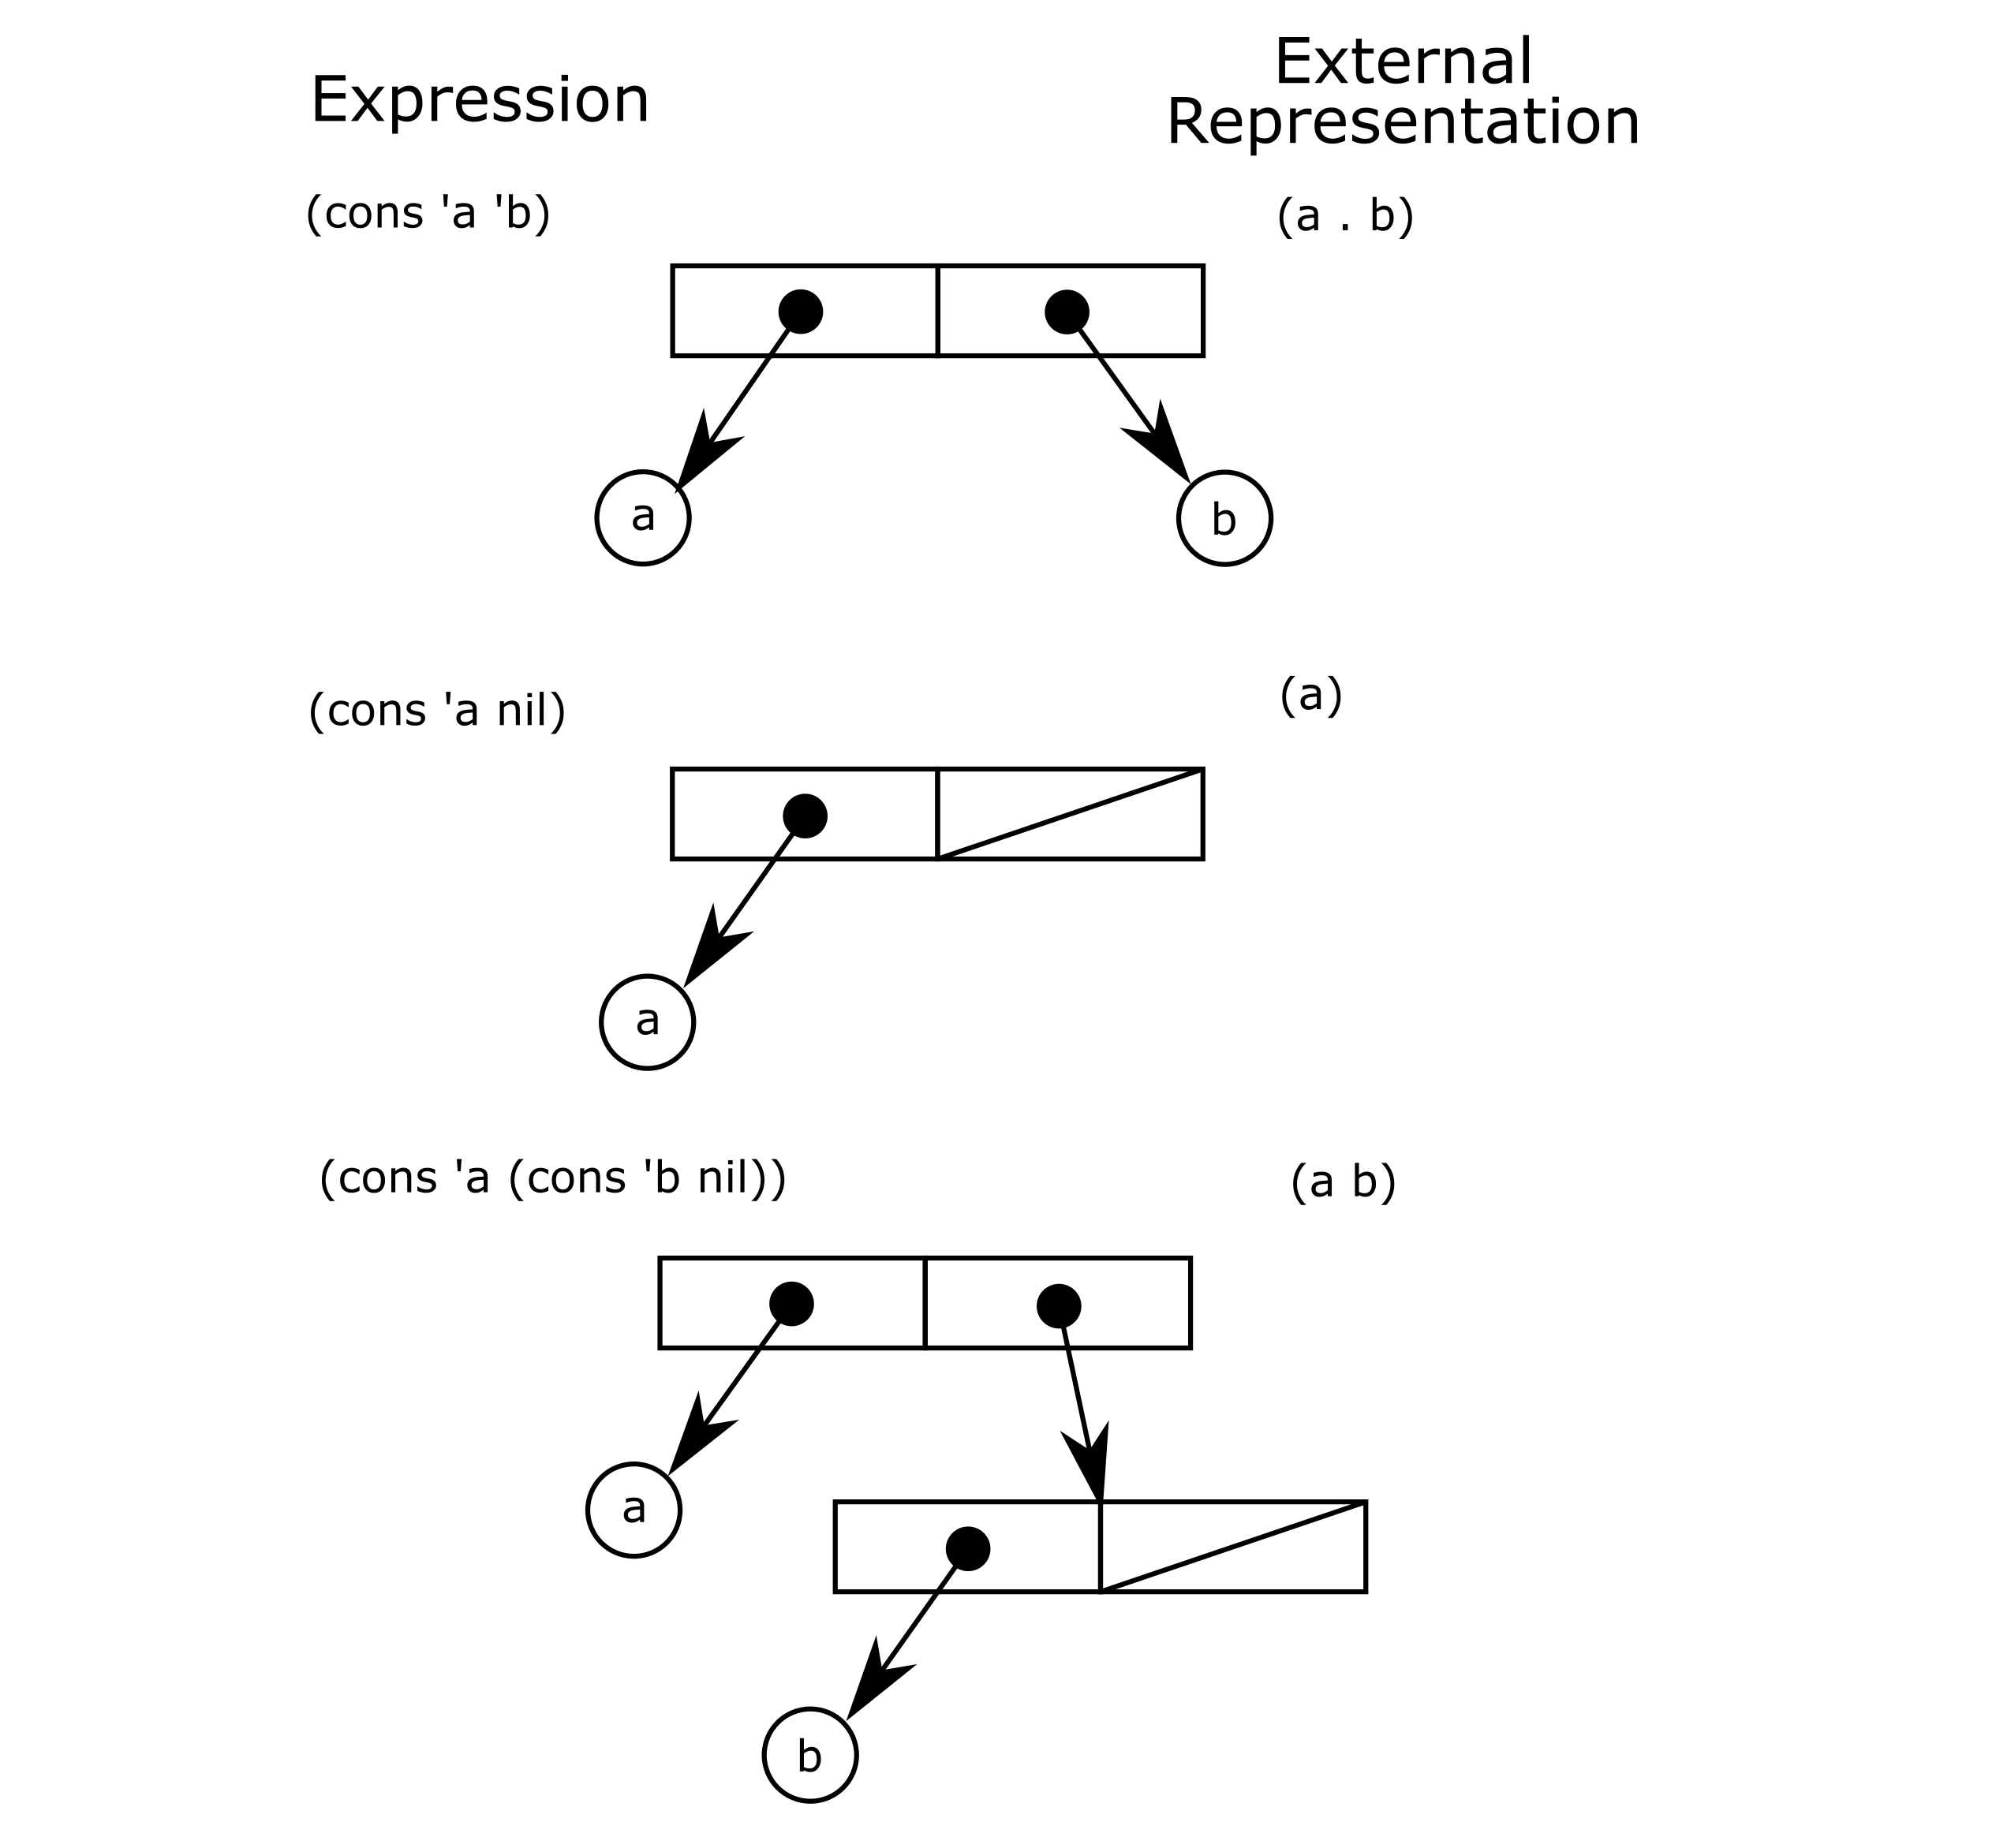
\includegraphics{images/consing.png}

\noindent\makebox[\linewidth]{\rule{\linewidth}{0.4pt}}
\begin{lstlisting}
reg cons
 
proc ::constcl::cons {car cdr} {
  MkPair $car $cdr
}
\end{lstlisting}
\noindent\makebox[\linewidth]{\rule{\linewidth}{0.4pt}}

\textbf{car}


\texttt{car} gets the contents of the first cell in a pair.

\begin{tabular}{ |l l| }
\hline
\multicolumn{2}{|l|}{car (public)} \\
\hline
pair & a pair \\
\textit{Returns:} & a Lisp value \\
\hline
\end{tabular}


Example:

\noindent\makebox[\linewidth]{\rule{\linewidth}{0.4pt}}
\begin{lstlisting}
(car '(a b))   =>  a
\end{lstlisting}
\noindent\makebox[\linewidth]{\rule{\linewidth}{0.4pt}}
\noindent\makebox[\linewidth]{\rule{\linewidth}{0.4pt}}
\begin{lstlisting}
reg car
 
proc ::constcl::car {pair} {
  $pair car
}
\end{lstlisting}
\noindent\makebox[\linewidth]{\rule{\linewidth}{0.4pt}}

\textbf{cdr}


\texttt{cdr} gets the contents of the second cell in a pair.

\begin{tabular}{ |l l| }
\hline
\multicolumn{2}{|l|}{cdr (public)} \\
\hline
pair & a pair \\
\textit{Returns:} & a Lisp value \\
\hline
\end{tabular}


Example:

\noindent\makebox[\linewidth]{\rule{\linewidth}{0.4pt}}
\begin{lstlisting}
(cdr '(a b))   =>  (b)
\end{lstlisting}
\noindent\makebox[\linewidth]{\rule{\linewidth}{0.4pt}}
\noindent\makebox[\linewidth]{\rule{\linewidth}{0.4pt}}
\begin{lstlisting}
reg cdr
 
proc ::constcl::cdr {pair} {
  $pair cdr
}
\end{lstlisting}
\noindent\makebox[\linewidth]{\rule{\linewidth}{0.4pt}}

\textbf{caar} to \textbf{cddddr}


\texttt{car} and \texttt{cdr} can be combined to form 28 composite access operations.

\noindent\makebox[\linewidth]{\rule{\linewidth}{0.4pt}}
\begin{lstlisting}
foreach ads {
  aa
  ad
  da
  dd
  aaa
  ada
  daa
  dda
  aad
  add
  dad
  ddd
  aaaa
  adaa
  daaa
  ddaa
  aada
  adda
  dada
  ddda
  aaad
  adad
  daad
  ddad
  aadd
  addd
  dadd
  dddd
} {
    reg c${ads}r
 
    proc ::constcl::c${ads}r {pair} "
        foreach c \[lreverse \[split $ads {}\]\] {
            if {\$c eq \"a\"} {
                set pair \[car \$pair\]
            } else {
                set pair \[cdr \$pair\]
            }
        }
        return \$pair
    "
 
}
\end{lstlisting}
\noindent\makebox[\linewidth]{\rule{\linewidth}{0.4pt}}

\textbf{set-car!}


\texttt{set-car!} sets the contents of the first cell in a pair.

\begin{tabular}{ |l l| }
\hline
\multicolumn{2}{|l|}{set-car! (public)} \\
\hline
pair & a pair \\
val & a Lisp value \\
\textit{Returns:} & a pair \\
\hline
\end{tabular}


Example:

\noindent\makebox[\linewidth]{\rule{\linewidth}{0.4pt}}
\begin{lstlisting}
(let ((pair (cons 'a 'b)) (val 'x))
  (set-car! pair val))                =>  (x . b)
\end{lstlisting}
\noindent\makebox[\linewidth]{\rule{\linewidth}{0.4pt}}
\noindent\makebox[\linewidth]{\rule{\linewidth}{0.4pt}}
\begin{lstlisting}
reg set-car!
 
proc ::constcl::set-car! {pair val} {
  $pair set-car! $val
}
\end{lstlisting}
\noindent\makebox[\linewidth]{\rule{\linewidth}{0.4pt}}

\textbf{set-cdr!}


\texttt{set-cdr!} sets the contents of the second cell in a pair.

\begin{tabular}{ |l l| }
\hline
\multicolumn{2}{|l|}{set-cdr! (public)} \\
\hline
pair & a pair \\
val & a Lisp value \\
\textit{Returns:} & a pair \\
\hline
\end{tabular}


Example:

\noindent\makebox[\linewidth]{\rule{\linewidth}{0.4pt}}
\begin{lstlisting}
(let ((pair (cons 'a 'b)) (val 'x))
  (set-cdr! pair val))                =>  (a . x)
\end{lstlisting}
\noindent\makebox[\linewidth]{\rule{\linewidth}{0.4pt}}
\noindent\makebox[\linewidth]{\rule{\linewidth}{0.4pt}}
\begin{lstlisting}
reg set-cdr!
 
proc ::constcl::set-cdr! {pair val} {
  $pair set-cdr! $val
}
\end{lstlisting}
\noindent\makebox[\linewidth]{\rule{\linewidth}{0.4pt}}

\textbf{list?}


The \texttt{list?} predicate tests if a pair is part of a proper list, one that ends with NIL.

\begin{tabular}{ |l l| }
\hline
\multicolumn{2}{|l|}{list? (public)} \\
\hline
val & a Lisp value \\
\textit{Returns:} & a boolean \\
\hline
\end{tabular}

\noindent\makebox[\linewidth]{\rule{\linewidth}{0.4pt}}
\begin{lstlisting}
reg list?
 
proc ::constcl::list? {val} {
  set visited {}
  if {[null? $val] ne "#f"} {
      return #t
  } elseif {[pair? $val] ne "#f"} {
      return [listp $val]
  } else {
      return #f
  }
}
\end{lstlisting}
\noindent\makebox[\linewidth]{\rule{\linewidth}{0.4pt}}
\begin{tabular}{ |l l| }
\hline
\multicolumn{2}{|l|}{listp (internal)} \\
\hline
pair & a pair \\
\textit{Returns:} & a boolean \\
\hline
\end{tabular}

\noindent\makebox[\linewidth]{\rule{\linewidth}{0.4pt}}
\begin{lstlisting}
proc ::constcl::listp {pair} {
  upvar visited visited
  if {$pair in $visited} {
    return #f
  }
  lappend visited $pair
  if {[null? $pair] ne "#f"} {
    return #t
  } elseif {[pair? $pair] ne "#f"} {
    return [listp [cdr $pair]]
  } else {
    return #f
  }
}
\end{lstlisting}
\noindent\makebox[\linewidth]{\rule{\linewidth}{0.4pt}}

\textbf{list}


\texttt{list} constructs a Lisp list from a number of values.

\begin{tabular}{ |l l| }
\hline
\multicolumn{2}{|l|}{list (public)} \\
\hline
args & some Lisp values \\
\textit{Returns:} & a Lisp list of Lisp values \\
\hline
\end{tabular}


Example:

\noindent\makebox[\linewidth]{\rule{\linewidth}{0.4pt}}
\begin{lstlisting}
(list 1 2 3)   =>  (1 2 3)
\end{lstlisting}
\noindent\makebox[\linewidth]{\rule{\linewidth}{0.4pt}}
\noindent\makebox[\linewidth]{\rule{\linewidth}{0.4pt}}
\begin{lstlisting}
reg list
 
proc ::constcl::list {args} {
  if {[llength $args] == 0} {
    return #NIL
  } else {
    set prev #NIL
    foreach obj [lreverse $args] {
      set prev [cons $obj $prev]
    }
    return $prev
  }
}
\end{lstlisting}
\noindent\makebox[\linewidth]{\rule{\linewidth}{0.4pt}}

\textbf{length}


\texttt{length} reports the length of a Lisp list.

\begin{tabular}{ |l l| }
\hline
\multicolumn{2}{|l|}{length (public)} \\
\hline
pair & a pair \\
\textit{Returns:} & a number \\
\hline
\end{tabular}


Example:

\noindent\makebox[\linewidth]{\rule{\linewidth}{0.4pt}}
\begin{lstlisting}
(length '(a b c d))   =>  4
\end{lstlisting}
\noindent\makebox[\linewidth]{\rule{\linewidth}{0.4pt}}
\noindent\makebox[\linewidth]{\rule{\linewidth}{0.4pt}}
\begin{lstlisting}
reg length
 
proc ::constcl::length {pair} {
  check {list? $pair} {
    LIST expected\n([pn] lst)
  }
  MkNumber [length-helper $pair]
}
\end{lstlisting}
\noindent\makebox[\linewidth]{\rule{\linewidth}{0.4pt}}
\begin{tabular}{ |l l| }
\hline
\multicolumn{2}{|l|}{length-helper (internal)} \\
\hline
pair & a pair \\
\textit{Returns:} & a Tcl number \\
\hline
\end{tabular}

\noindent\makebox[\linewidth]{\rule{\linewidth}{0.4pt}}
\begin{lstlisting}
proc ::constcl::length-helper {pair} {
  if {[null? $pair] ne "#f"} {
    return 0
  } else {
    return [expr {1 +
      [length-helper [cdr $pair]]}]
  }
}
\end{lstlisting}
\noindent\makebox[\linewidth]{\rule{\linewidth}{0.4pt}}

\textbf{append}


\texttt{append} joins lists together.


Example:

\noindent\makebox[\linewidth]{\rule{\linewidth}{0.4pt}}
\begin{lstlisting}
(append '(a b) '(c d))   =>  (a b c d)
\end{lstlisting}
\noindent\makebox[\linewidth]{\rule{\linewidth}{0.4pt}}
\begin{tabular}{ |l l| }
\hline
\multicolumn{2}{|l|}{append (public)} \\
\hline
args & some lists \\
\textit{Returns:} & a Lisp list of Lisp values \\
\hline
\end{tabular}

\noindent\makebox[\linewidth]{\rule{\linewidth}{0.4pt}}
\begin{lstlisting}
reg append
 
proc ::constcl::append {args} {
  set prev [lindex $args end]
  foreach r [lreverse [lrange $args 0 end-1]] {
    check {list? $r} {
      LIST expected\n([pn] [$r show])
    }
    set prev [copy-list $r $prev]
  }
  set prev
}
\end{lstlisting}
\noindent\makebox[\linewidth]{\rule{\linewidth}{0.4pt}}
\begin{tabular}{ |l l| }
\hline
\multicolumn{2}{|l|}{copy-list (internal)} \\
\hline
pair & a pair \\
next & a Lisp list of Lisp values \\
\textit{Returns:} & a Lisp list of Lisp values \\
\hline
\end{tabular}

\noindent\makebox[\linewidth]{\rule{\linewidth}{0.4pt}}
\begin{lstlisting}
proc ::constcl::copy-list {pair next} {
  # TODO only fresh conses in the direct chain to NIL
  if {[null? $pair] ne "#f"} {
    set next
  } elseif {[null? [cdr $pair]] ne "#f"} {
    cons [car $pair] $next
  } else {
    cons [car $pair] [copy-list [cdr $pair] $next]
  }
}
\end{lstlisting}
\noindent\makebox[\linewidth]{\rule{\linewidth}{0.4pt}}

\textbf{reverse}


\texttt{reverse} produces a reversed copy of a Lisp list.

\begin{tabular}{ |l l| }
\hline
\multicolumn{2}{|l|}{reverse (public)} \\
\hline
vals & a Lisp list of Lisp values \\
\textit{Returns:} & a Lisp list of Lisp values \\
\hline
\end{tabular}


Example:

\noindent\makebox[\linewidth]{\rule{\linewidth}{0.4pt}}
\begin{lstlisting}
(reverse '(a b c))   =>  (c b a)
\end{lstlisting}
\noindent\makebox[\linewidth]{\rule{\linewidth}{0.4pt}}
\noindent\makebox[\linewidth]{\rule{\linewidth}{0.4pt}}
\begin{lstlisting}
reg reverse
 
proc ::constcl::reverse {vals} {
  list {*}[lreverse [splitlist $vals]]
}
\end{lstlisting}
\noindent\makebox[\linewidth]{\rule{\linewidth}{0.4pt}}

\textbf{list-tail}


Given a list index, \texttt{list-tail} yields the sublist starting from that index.

\begin{tabular}{ |l l| }
\hline
\multicolumn{2}{|l|}{list-tail (public)} \\
\hline
vals & a Lisp list of Lisp values \\
k & a number \\
\textit{Returns:} & a Lisp list of Lisp values \\
\hline
\end{tabular}


Example:

\noindent\makebox[\linewidth]{\rule{\linewidth}{0.4pt}}
\begin{lstlisting}
(let ((lst '(a b c d e f)) (k 3))
  (list-tail lst k))                =>  (d e f)
\end{lstlisting}
\noindent\makebox[\linewidth]{\rule{\linewidth}{0.4pt}}
\noindent\makebox[\linewidth]{\rule{\linewidth}{0.4pt}}
\begin{lstlisting}
reg list-tail
 
proc ::constcl::list-tail {vals k} {
  if {[zero? $k] ne "#f"} {
    return $vals
  } else {
    list-tail [cdr $vals] [- $k #1]
  }
}
\end{lstlisting}
\noindent\makebox[\linewidth]{\rule{\linewidth}{0.4pt}}

\textbf{list-ref}


\texttt{list-ref} yields the list item at a given index.

\begin{tabular}{ |l l| }
\hline
\multicolumn{2}{|l|}{list-ref (public)} \\
\hline
vals & a Lisp list of Lisp values \\
k & a number \\
\textit{Returns:} & a Lisp value \\
\hline
\end{tabular}


Example:

\noindent\makebox[\linewidth]{\rule{\linewidth}{0.4pt}}
\begin{lstlisting}
(let ((lst '(a b c d e f)) (k 3))
  (list-ref lst k))                 =>  d
\end{lstlisting}
\noindent\makebox[\linewidth]{\rule{\linewidth}{0.4pt}}
\noindent\makebox[\linewidth]{\rule{\linewidth}{0.4pt}}
\begin{lstlisting}
reg list-ref
 
proc ::constcl::list-ref {vals k} {
  car [list-tail $vals $k]
}
\end{lstlisting}
\noindent\makebox[\linewidth]{\rule{\linewidth}{0.4pt}}

\textbf{memq}


\textbf{memv}


\textbf{member}


\texttt{memq}, \texttt{memv}, and \texttt{member} return the sublist starting with a given item, or \texttt{\#f} if there is none. They use \texttt{eq?}, \texttt{eqv?}, and \texttt{equal?}, respectively, for the comparison.

\begin{tabular}{ |l l| }
\hline
\multicolumn{2}{|l|}{memq (public)} \\
\hline
val1 & a Lisp value \\
val2 & a Lisp list of Lisp values \\
\textit{Returns:} & a Lisp list of values OR \#f \\
\hline
\end{tabular}


Example:

\noindent\makebox[\linewidth]{\rule{\linewidth}{0.4pt}}
\begin{lstlisting}
(let ((lst '(a b c d e f)) (val 'd))
  (memq val lst))                      =>  (d e f)
\end{lstlisting}
\noindent\makebox[\linewidth]{\rule{\linewidth}{0.4pt}}
\noindent\makebox[\linewidth]{\rule{\linewidth}{0.4pt}}
\begin{lstlisting}
reg memq
 
proc ::constcl::memq {val1 val2} {
  return [member-proc eq? $val1 $val2]
}
\end{lstlisting}
\noindent\makebox[\linewidth]{\rule{\linewidth}{0.4pt}}
\begin{tabular}{ |l l| }
\hline
\multicolumn{2}{|l|}{memv (public)} \\
\hline
val1 & a Lisp value \\
val2 & a Lisp list of Lisp values \\
\textit{Returns:} & a Lisp list of values OR \#f \\
\hline
\end{tabular}

\noindent\makebox[\linewidth]{\rule{\linewidth}{0.4pt}}
\begin{lstlisting}
reg memv
 
proc ::constcl::memv {val1 val2} {
  return [member-proc eqv? $val1 $val2]
}
\end{lstlisting}
\noindent\makebox[\linewidth]{\rule{\linewidth}{0.4pt}}
\begin{tabular}{ |l l| }
\hline
\multicolumn{2}{|l|}{member (public)} \\
\hline
val1 & a Lisp value \\
val2 & a Lisp list of Lisp values \\
\textit{Returns:} & a Lisp list of values OR \#f \\
\hline
\end{tabular}

\noindent\makebox[\linewidth]{\rule{\linewidth}{0.4pt}}
\begin{lstlisting}
reg member
 
proc ::constcl::member {val1 val2} {
  return [member-proc equal? $val1 $val2]
}
\end{lstlisting}
\noindent\makebox[\linewidth]{\rule{\linewidth}{0.4pt}}
\begin{tabular}{ |l l| }
\hline
\multicolumn{2}{|l|}{member-proc (internal)} \\
\hline
epred & an equivalence predicate \\
val1 & a Lisp value \\
val2 & a Lisp list of Lisp values \\
\textit{Returns:} & a Lisp list of values OR \#f \\
\hline
\end{tabular}

\noindent\makebox[\linewidth]{\rule{\linewidth}{0.4pt}}
\begin{lstlisting}
 
proc ::constcl::member-proc {epred val1 val2} {
  switch $epred {
    eq? { set name "memq" }
    eqv? { set name "memv" }
    equal? { set name "member" }
  }
  check {list? $val2} {
    LIST expected\n($name [$val1 show] [$val2 show])
  }
  if {[null? $val2] ne "#f"} {
    return #f
  } elseif {[pair? $val2] ne "#f"} {
    if {[$epred $val1 [car $val2]] ne "#f"} {
      return $val2
    } else {
      return [member-proc $epred $val1 [cdr $val2]]
    }
  }
}
\end{lstlisting}
\noindent\makebox[\linewidth]{\rule{\linewidth}{0.4pt}}

\textbf{assq}


\textbf{assv}


\textbf{assoc}


\texttt{assq}, \texttt{assv}, and \texttt{assoc} return the associative item marked with a given item, or \texttt{\#f} if there is none. They use \texttt{eq?}, \texttt{eqv?}, and \texttt{equal?}, respectively, for the comparison. They implement lookup in the form of lookup table known as an association list, or \_alist\_.


Example:

\noindent\makebox[\linewidth]{\rule{\linewidth}{0.4pt}}
\begin{lstlisting}
(define e '((a 1) (b 2) (c 3)))
(assq 'a e)                       => (a 1)
\end{lstlisting}
\noindent\makebox[\linewidth]{\rule{\linewidth}{0.4pt}}
\begin{tabular}{ |l l| }
\hline
\multicolumn{2}{|l|}{assq (public)} \\
\hline
val1 & a Lisp value \\
val2 & an association list \\
\textit{Returns:} & a Lisp list of values OR \#f \\
\hline
\end{tabular}

\noindent\makebox[\linewidth]{\rule{\linewidth}{0.4pt}}
\begin{lstlisting}
reg assq
 
proc ::constcl::assq {val1 val2} {
  return [assoc-proc eq? $val1 $val2]
}
\end{lstlisting}
\noindent\makebox[\linewidth]{\rule{\linewidth}{0.4pt}}
\begin{tabular}{ |l l| }
\hline
\multicolumn{2}{|l|}{assv (public)} \\
\hline
val1 & a Lisp value \\
val2 & an association list \\
\textit{Returns:} & a Lisp list of values OR \#f \\
\hline
\end{tabular}

\noindent\makebox[\linewidth]{\rule{\linewidth}{0.4pt}}
\begin{lstlisting}
reg assv
 
proc ::constcl::assv {val1 val2} {
  return [assoc-proc eqv? $val1 $val2]
}
\end{lstlisting}
\noindent\makebox[\linewidth]{\rule{\linewidth}{0.4pt}}
\begin{tabular}{ |l l| }
\hline
\multicolumn{2}{|l|}{assoc (public)} \\
\hline
val1 & a Lisp value \\
val2 & an association list \\
\textit{Returns:} & a Lisp list of values OR \#f \\
\hline
\end{tabular}

\noindent\makebox[\linewidth]{\rule{\linewidth}{0.4pt}}
\begin{lstlisting}
reg assoc
 
proc ::constcl::assoc {val1 val2} {
  return [assoc-proc equal? $val1 $val2]
}
\end{lstlisting}
\noindent\makebox[\linewidth]{\rule{\linewidth}{0.4pt}}
\begin{tabular}{ |l l| }
\hline
\multicolumn{2}{|l|}{assoc-proc (internal)} \\
\hline
epred & an equivalence predicate \\
val1 & a Lisp value \\
val2 & an association list \\
\textit{Returns:} & a Lisp list of values OR \#f \\
\hline
\end{tabular}

\noindent\makebox[\linewidth]{\rule{\linewidth}{0.4pt}}
\begin{lstlisting}
proc ::constcl::assoc-proc {epred val1 val2} {
  switch $epred {
    eq? { set name "assq" }
    eqv? { set name "assv" }
    equal? { set name "assoc" }
  }
  check {list? $val2} {
    LIST expected\n($name [$val1 show] [$val2 show])
  }
  if {[null? $val2] ne "#f"} {
    return #f
  } elseif {[pair? $val2] ne "#f"} {
    if {[pair? [car $val2]] ne "#f" && 
      [$epred $val1 [caar $val2]] ne "#f"} {
      return [car $val2]
    } else {
      return [assoc-proc $epred $val1 [cdr $val2]]
    }
  }
}
\end{lstlisting}
\noindent\makebox[\linewidth]{\rule{\linewidth}{0.4pt}}
\section{Strings}
\label{strings}

Procedures for dealing with strings of characters.


\textbf{String} class


Strings have the internal representation of a vector of character objects, with the data elements of the vector address of the first element, and the length of the vector. External representation is surrounded by double quotes, with double quotes and backslashes within the string escaped with a backslash.


As a ConsTcl extension, a backslash+n pair in the external representation is stored as a newline character. It is restored to backslash+n on write.

\noindent\makebox[\linewidth]{\rule{\linewidth}{0.4pt}}
\begin{lstlisting}
oo::class create ::constcl::String {
  superclass ::constcl::NIL
  variable data constant
  constructor {v} {
    set v [string map {\\\\ \\ \\\" \" \\n \n} $v]
    set len [::string length $v]
    set vsa [::constcl::vsAlloc $len]
    set idx $vsa
    foreach elt [split $v {}] {
      if {$elt eq " "} {
        set c #\\space
      } elseif {$elt eq "\n"} {
        set c #\\newline
      } else {
        set c #\\$elt
      }
      lset ::constcl::vectorSpace $idx \
        [::constcl::MkChar $c]
      incr idx
    }
    set data [
      ::constcl::cons [N $vsa] [N $len]]
    set constant 0
  }
  method = {str} {
    ::string equal [my value] [$str value]
  }
  method cmp {str} {
    ::string compare [my value] [$str value]
  }
  method length {} {
    ::constcl::cdr $data
  }
  method ref {k} {
    set k [$k numval]
    if {$k < 0 || $k >= [[my length] numval]} {
      ::error "index out of range\n$k"
    }
    lindex [my store] $k
  }
  method store {} {
    set base [[::constcl::car $data] numval]
    set end [expr {[[my length] numval] +
      $base - 1}]
    lrange $::constcl::vectorSpace $base $end
  }
  method value {} {
    join [lmap c [my store] {$c char}] {}
  }
  method set! {k c} {
    if {[my constant]} {
      ::error "string is constant"
    } else {
      set k [$k numval]
      if {$k < 0 ||
        $k >= [[my length] numval]} {
        ::error "index out of range\n$k"
      }
      set base [[::constcl::car $data] numval]
      lset ::constcl::vectorSpace $k+$base $c
    }
    return [self]
  }
  method fill! {c} {
    if {[my constant]} {
      ::error "string is constant"
    } else {
      set base [[::constcl::car $data] numval]
      set len [[my length] numval]
      for {set idx $base} \
        {$idx < $len+$base} \
        {incr idx} {
        lset ::constcl::vectorSpace $idx $c
      }
    }
    return [self]
  }
  method substring {from to} {
    join [lmap c [lrange [my store] \
      [$from numval] [$to numval]] {$c char}] {}
  }
  method mkconstant {} {
    set constant 1
  }
  method constant {} {
    set constant
  }
  method external {} {
    return "\"[
      string map {\\ \\\\ \" \\\" \n \\n} [my value]]\""
  }
  method write {handle} {
    puts -nonewline $handle [my external]
  }
  method display {handle} {
    puts -nonewline $handle [my value]
  }
  method show {} {
    my external
  }
}
 
interp alias {} ::constcl::MkString \
  {} ::constcl::String new
\end{lstlisting}
\noindent\makebox[\linewidth]{\rule{\linewidth}{0.4pt}}
\begin{tabular}{ |l l| }
\hline
\multicolumn{2}{|l|}{string? (public)} \\
\hline
val & a Lisp value \\
\textit{Returns:} & a boolean \\
\hline
\end{tabular}

\noindent\makebox[\linewidth]{\rule{\linewidth}{0.4pt}}
\begin{lstlisting}
reg string?
 
proc ::constcl::string? {val} {
  typeof? $val String
}
\end{lstlisting}
\noindent\makebox[\linewidth]{\rule{\linewidth}{0.4pt}}

\textbf{make-string}


\texttt{make-string} creates a string of \emph{k} characters, optionally filled with \emph{char} characters. If \emph{char} is omitted, the string will be filled with space characters.

\begin{tabular}{ |l l| }
\hline
\multicolumn{2}{|l|}{make-string (public)} \\
\hline
k & a number \\
?char? & a character \\
\textit{Returns:} & a string \\
\hline
\end{tabular}


Example:

\noindent\makebox[\linewidth]{\rule{\linewidth}{0.4pt}}
\begin{lstlisting}
(let ((k 5))
  (make-string k))        =>  "     "
(let ((k 5) (char #\A))
  (make-string k char))   =>  "AAAAA"
\end{lstlisting}
\noindent\makebox[\linewidth]{\rule{\linewidth}{0.4pt}}
\noindent\makebox[\linewidth]{\rule{\linewidth}{0.4pt}}
\begin{lstlisting}
reg make-string
 
proc ::constcl::make-string {k args} {
  if {[llength $args] == 0} {
    return [MkString [::string repeat " " \
      [$k numval]]]
  } else {
    lassign $args char
    return [MkString [::string repeat \
      [$char char] [$k numval]]]
  }
}
\end{lstlisting}
\noindent\makebox[\linewidth]{\rule{\linewidth}{0.4pt}}

\textbf{string}


\texttt{string} constructs a string from a number of Lisp characters.

\begin{tabular}{ |l l| }
\hline
\multicolumn{2}{|l|}{string (public)} \\
\hline
args & some characters \\
\textit{Returns:} & a string \\
\hline
\end{tabular}


Example:

\noindent\makebox[\linewidth]{\rule{\linewidth}{0.4pt}}
\begin{lstlisting}
(string #\f #\o #\o)   =>  "foo"
\end{lstlisting}
\noindent\makebox[\linewidth]{\rule{\linewidth}{0.4pt}}
\noindent\makebox[\linewidth]{\rule{\linewidth}{0.4pt}}
\begin{lstlisting}
reg string
 
proc ::constcl::string {args} {
  set str {}
  foreach char $args {
    check {::constcl::char? $char} {
      CHAR expected\n([pn] [lmap c $args \
        {$c show}])
    }
    ::append str [$char char]
  }
  return [MkString $str]
}
\end{lstlisting}
\noindent\makebox[\linewidth]{\rule{\linewidth}{0.4pt}}

\textbf{string-length}


\texttt{string-length} reports a string's length.

\begin{tabular}{ |l l| }
\hline
\multicolumn{2}{|l|}{string-length (public)} \\
\hline
str & a string \\
\textit{Returns:} & a number \\
\hline
\end{tabular}


Example:

\noindent\makebox[\linewidth]{\rule{\linewidth}{0.4pt}}
\begin{lstlisting}
(string-length "foobar")   => 6
\end{lstlisting}
\noindent\makebox[\linewidth]{\rule{\linewidth}{0.4pt}}
\noindent\makebox[\linewidth]{\rule{\linewidth}{0.4pt}}
\begin{lstlisting}
reg string-length
 
proc ::constcl::string-length {str} {
  check {::constcl::string? $str} {
    STRING expected\n([pn] [$str show])
  }
  return [MkNumber [[$str length] numval]]
}
\end{lstlisting}
\noindent\makebox[\linewidth]{\rule{\linewidth}{0.4pt}}

\textbf{string-ref}


\texttt{string-ref} yields the \_k\_-th character (0-based) in \_str\_.

\begin{tabular}{ |l l| }
\hline
\multicolumn{2}{|l|}{string-ref (public)} \\
\hline
str & a string \\
k & a number \\
\textit{Returns:} & a character \\
\hline
\end{tabular}


Example:

\noindent\makebox[\linewidth]{\rule{\linewidth}{0.4pt}}
\begin{lstlisting}
(string-ref "foobar" 3)   => #\b
\end{lstlisting}
\noindent\makebox[\linewidth]{\rule{\linewidth}{0.4pt}}
\noindent\makebox[\linewidth]{\rule{\linewidth}{0.4pt}}
\begin{lstlisting}
reg string-ref
 
proc ::constcl::string-ref {str k} {
  check {::constcl::string? $str} {
    STRING expected\n([pn] [$str show] \
      [$k show])
  }
  check {::constcl::number? $k} {
    Exact INTEGER expected\n([pn] [$str show] \
      [$k show])
  }
  return [$str ref $k]
}
\end{lstlisting}
\noindent\makebox[\linewidth]{\rule{\linewidth}{0.4pt}}

\textbf{string-set!}


\texttt{string-set!} replaces the character at \_k\_ with \_char\_ in a non-constant string.

\begin{tabular}{ |l l| }
\hline
\multicolumn{2}{|l|}{string-set! (public)} \\
\hline
str & a string \\
k & a number \\
char & a character \\
\textit{Returns:} & a string \\
\hline
\end{tabular}


Example:

\noindent\makebox[\linewidth]{\rule{\linewidth}{0.4pt}}
\begin{lstlisting}
(let ((str (string #\f #\o #\o))
      (k 2)
      (char #\x))
  (string-set! str k char))         =>  "fox"
\end{lstlisting}
\noindent\makebox[\linewidth]{\rule{\linewidth}{0.4pt}}
\noindent\makebox[\linewidth]{\rule{\linewidth}{0.4pt}}
\begin{lstlisting}
reg string-set!
 
proc ::constcl::string-set! {str k char} {
  check {string? $str} {
    STRING expected\n([pn] [$str show] [$k show] \
      [$char show])
  }
  check {number? $k} {
    Exact INTEGER expected\n([pn] [$str show] \
      [$k show] [$char show])
  }
  check {char? $char} {
    CHAR expected\n([pn] [$str show] [$k show] \
      [$char show])
  }
  $str set! $k $char
  return $str
}
\end{lstlisting}
\noindent\makebox[\linewidth]{\rule{\linewidth}{0.4pt}}

\textbf{string=?}, \textbf{string-ci=?}


\textbf{string<?}, \textbf{string-ci<?}


\textbf{string>?}, \textbf{string-ci>?}


\textbf{string<=?}, \textbf{string-ci<=?}


\textbf{string>=?}, \textbf{string-ci>=?}


\texttt{string=?}, \texttt{string<?}, \texttt{string>?}, \texttt{string<=?}, \texttt{string>=?} and their case insensitive variants \texttt{string-ci=?}, \texttt{string-ci<?}, \texttt{string-ci>?}, \texttt{string-ci<=?}, \texttt{string-ci>=?} compare strings.

\begin{tabular}{ |l l| }
\hline
\multicolumn{2}{|l|}{string=?, string<?, string>?, string<=?, string>=? (public)} \\
\hline
str1 & a string \\
str2 & a string \\
\textit{Returns:} & a boolean \\
\hline
\end{tabular}

\begin{tabular}{ |l l| }
\hline
\multicolumn{2}{|l|}{string-ci=?, string-ci<?, string-ci>? (public)} \\
\hline
str1 & a string \\
str2 & a string \\
\textit{Returns:} & a boolean \\
\hline
\end{tabular}

\begin{tabular}{ |l l| }
\hline
\multicolumn{2}{|l|}{string-ci<=?, string-ci>=? (public)} \\
\hline
str1 & a string \\
str2 & a string \\
\textit{Returns:} & a boolean \\
\hline
\end{tabular}

\noindent\makebox[\linewidth]{\rule{\linewidth}{0.4pt}}
\begin{lstlisting}
reg string=?
 
proc ::constcl::string=? {str1 str2} {
  check {string? $str1} {
    STRING expected\n([pn] [$str1 show] \
      [$str2 show])
  }
  check {string? $str2} {
    STRING expected\n([pn] [$str1 show] \
      [$str2 show])
  }
  if {[$str1 value] eq [$str2 value]} {
    return #t
  } else {
    return #f
  }
}
\end{lstlisting}
\noindent\makebox[\linewidth]{\rule{\linewidth}{0.4pt}}
\noindent\makebox[\linewidth]{\rule{\linewidth}{0.4pt}}
\begin{lstlisting}
reg string-ci=?
 
proc ::constcl::string-ci=? {str1 str2} {
  check {string? $str1} {
    STRING expected\n([pn] [$str1 show] \
      [$str2 show])
  }
  check {string? $str2} {
    STRING expected\n([pn] [$str1 show] \
      [$str2 show])
  }
  if {[::string tolower [$str1 value]] eq
      [::string tolower [$str2 value]]} {
    return #t
  } else {
    return #f
  }
}
\end{lstlisting}
\noindent\makebox[\linewidth]{\rule{\linewidth}{0.4pt}}
\noindent\makebox[\linewidth]{\rule{\linewidth}{0.4pt}}
\begin{lstlisting}
reg string<?
 
proc ::constcl::string<? {str1 str2} {
  check {string? $str1} {
    STRING expected\n([pn] [$str1 show] \
      [$str2 show])
  }
  check {string? $str2} {
    STRING expected\n([pn] [$str1 show] \
      [$str2 show])
  }
  if {[$str1 value] < [$str2 value]} {
    return #t
  } else {
    return #f
  }
}
\end{lstlisting}
\noindent\makebox[\linewidth]{\rule{\linewidth}{0.4pt}}
\noindent\makebox[\linewidth]{\rule{\linewidth}{0.4pt}}
\begin{lstlisting}
reg string-ci<?
 
proc ::constcl::string-ci<? {str1 str2} {
  check {string? $str1} {
    STRING expected\n([pn] [$str1 show] \
      [$str2 show])
  }
  check {string? $str2} {
    STRING expected\n([pn] [$str1 show] \
      [$str2 show])
  }
  if {[::string tolower [$str1 value]] <
      [::string tolower [$str2 value]]} {
    return #t
  } else {
    return #f
  }
}
\end{lstlisting}
\noindent\makebox[\linewidth]{\rule{\linewidth}{0.4pt}}
\noindent\makebox[\linewidth]{\rule{\linewidth}{0.4pt}}
\begin{lstlisting}
reg string>?
 
proc ::constcl::string>? {str1 str2} {
  check {string? $str1} {
    STRING expected\n([pn] [$str1 show] \
      [$str2 show])
  }
  check {string? $str2} {
    STRING expected\n([pn] [$str1 show] \
      [$str2 show])
  }
  if {[$str1 value] > [$str2 value]} {
    return #t
  } else {
    return #f
  }
}
\end{lstlisting}
\noindent\makebox[\linewidth]{\rule{\linewidth}{0.4pt}}
\noindent\makebox[\linewidth]{\rule{\linewidth}{0.4pt}}
\begin{lstlisting}
reg string-ci>?
 
proc ::constcl::string-ci>? {str1 str2} {
  check {string? $str1} {
    STRING expected\n([pn] [$str1 show] \
      [$str2 show])
  }
  check {string? $str2} {
    STRING expected\n([pn] [$str1 show] \
      [$str2 show])
  }
  if {[::string tolower [$str1 value]] >
      [::string tolower [$str2 value]]} {
    return #t
  } else {
    return #f
  }
}
\end{lstlisting}
\noindent\makebox[\linewidth]{\rule{\linewidth}{0.4pt}}
\noindent\makebox[\linewidth]{\rule{\linewidth}{0.4pt}}
\begin{lstlisting}
reg string<=?
 
proc ::constcl::string<=? {str1 str2} {
  check {string? $str1} {
    STRING expected\n([pn] [$str1 show] \
      [$str2 show])
  }
  check {string? $str2} {
    STRING expected\n([pn] [$str1 show] \
      [$str2 show])
  }
  if {[$str1 value] <= [$str2 value]} {
    return #t
  } else {
    return #f
  }
}
\end{lstlisting}
\noindent\makebox[\linewidth]{\rule{\linewidth}{0.4pt}}
\noindent\makebox[\linewidth]{\rule{\linewidth}{0.4pt}}
\begin{lstlisting}
reg string-ci<=?
 
proc ::constcl::string-ci<=? {str1 str2} {
  check {string? $str1} {
    STRING expected\n([pn] [$str1 show] \
      [$str2 show])
  }
  check {string? $str2} {
    STRING expected\n([pn] [$str1 show] \
      [$str2 show])
  }
  if {[::string tolower [$str1 value]] <=
      [::string tolower [$str2 value]]} {
    return #t
  } else {
    return #f
  }
}
\end{lstlisting}
\noindent\makebox[\linewidth]{\rule{\linewidth}{0.4pt}}
\noindent\makebox[\linewidth]{\rule{\linewidth}{0.4pt}}
\begin{lstlisting}
reg string>=?
 
proc ::constcl::string>=? {str1 str2} {
  check {string? $str1} {
    STRING expected\n([pn] [$str1 show] \
      [$str2 show])
  }
  check {string? $str2} {
    STRING expected\n([pn] [$str1 show] \
      [$str2 show])
  }
  if {[$str1 value] >= [$str2 value]} {
    return #t
  } else {
    return #f
  }
}
\end{lstlisting}
\noindent\makebox[\linewidth]{\rule{\linewidth}{0.4pt}}
\noindent\makebox[\linewidth]{\rule{\linewidth}{0.4pt}}
\begin{lstlisting}
reg string-ci>=?
 
proc ::constcl::string-ci>=? {str1 str2} {
  check {string? $str1} {
    STRING expected\n([pn] [$str1 show] \
      [$str2 show])
  }
  check {string? $str2} {
    STRING expected\n([pn] [$str1 show] \
      [$str2 show])
  }
  if {[::string tolower [$str1 value]] >=
      [::string tolower [$str2 value]]} {
    return #t
  } else {
    return #f
  }
}
\end{lstlisting}
\noindent\makebox[\linewidth]{\rule{\linewidth}{0.4pt}}

\textbf{substring}


\texttt{substring} yields the substring of \emph{str} that starts at \emph{start} and ends at \emph{end}.

\begin{tabular}{ |l l| }
\hline
\multicolumn{2}{|l|}{substring (public)} \\
\hline
str & a string \\
start & a number \\
end & a number \\
\textit{Returns:} & a string \\
\hline
\end{tabular}


Example:

\noindent\makebox[\linewidth]{\rule{\linewidth}{0.4pt}}
\begin{lstlisting}
(substring "foobar" 2 4)   => "oba"
\end{lstlisting}
\noindent\makebox[\linewidth]{\rule{\linewidth}{0.4pt}}
\noindent\makebox[\linewidth]{\rule{\linewidth}{0.4pt}}
\begin{lstlisting}
reg substring
 
proc ::constcl::substring {str start end} {
  check {string? $str} {
    STRING expected\n([pn] [$str show] \
      [$start show] [$end show])
  }
  check {number? $start} {
    NUMBER expected\n([pn] [$str show] \
      [$start show] [$end show])
  }
  check {number? $end} {
    NUMBER expected\n([pn] [$str show] \
      [$start show] [$end show])
  }
  return [MkString [$str substring $start $end]]
}
\end{lstlisting}
\noindent\makebox[\linewidth]{\rule{\linewidth}{0.4pt}}

\textbf{string-append}


\texttt{string-append} joins strings together.

\begin{tabular}{ |l l| }
\hline
\multicolumn{2}{|l|}{string-append (public)} \\
\hline
args & some strings \\
\textit{Returns:} & a string \\
\hline
\end{tabular}


Example:

\noindent\makebox[\linewidth]{\rule{\linewidth}{0.4pt}}
\begin{lstlisting}
(string-append "foo" "bar")   =>  "foobar"
\end{lstlisting}
\noindent\makebox[\linewidth]{\rule{\linewidth}{0.4pt}}
\noindent\makebox[\linewidth]{\rule{\linewidth}{0.4pt}}
\begin{lstlisting}
reg string-append
 
proc ::constcl::string-append {args} {
    MkString [::append --> {*}[lmap arg $args {
      $arg value
    }]]
}
\end{lstlisting}
\noindent\makebox[\linewidth]{\rule{\linewidth}{0.4pt}}

\textbf{string->list}


\texttt{string->list} converts a string to a Lisp list of characters.

\begin{tabular}{ |l l| }
\hline
\multicolumn{2}{|l|}{string->list (public)} \\
\hline
str & a string \\
\textit{Returns:} & a Lisp list of characters \\
\hline
\end{tabular}


Example:

\noindent\makebox[\linewidth]{\rule{\linewidth}{0.4pt}}
\begin{lstlisting}
(string->list "foo")   =>  (#\f #\o #\o)
\end{lstlisting}
\noindent\makebox[\linewidth]{\rule{\linewidth}{0.4pt}}
\noindent\makebox[\linewidth]{\rule{\linewidth}{0.4pt}}
\begin{lstlisting}
reg string->list
 
proc ::constcl::string->list {str} {
  list {*}[$str store]
}
\end{lstlisting}
\noindent\makebox[\linewidth]{\rule{\linewidth}{0.4pt}}

\textbf{list->string}


\texttt{list->string} converts a Lisp list of characters to a string.

\begin{tabular}{ |l l| }
\hline
\multicolumn{2}{|l|}{list->string (public)} \\
\hline
list & a Lisp list of characters \\
\textit{Returns:} & a string \\
\hline
\end{tabular}


Example:

\noindent\makebox[\linewidth]{\rule{\linewidth}{0.4pt}}
\begin{lstlisting}
(list->string '(#\1 #\2 #\3))   => "123"
\end{lstlisting}
\noindent\makebox[\linewidth]{\rule{\linewidth}{0.4pt}}
\noindent\makebox[\linewidth]{\rule{\linewidth}{0.4pt}}
\begin{lstlisting}
reg list->string
 
proc ::constcl::list->string {list} {
  MkString [::append --> {*}[
    lmap c [splitlist $list] {$c char}]]
}
\end{lstlisting}
\noindent\makebox[\linewidth]{\rule{\linewidth}{0.4pt}}

\textbf{string-copy}


\texttt{string-copy} makes a copy of a string.

\begin{tabular}{ |l l| }
\hline
\multicolumn{2}{|l|}{string-copy (public)} \\
\hline
str & a string \\
\textit{Returns:} & a string \\
\hline
\end{tabular}


Example:

\noindent\makebox[\linewidth]{\rule{\linewidth}{0.4pt}}
\begin{lstlisting}
(let ((str (string-copy "abc"))
      (k 0)
      (char #\x))
  (string-set! str k char))       =>  "xbc"
\end{lstlisting}
\noindent\makebox[\linewidth]{\rule{\linewidth}{0.4pt}}
\noindent\makebox[\linewidth]{\rule{\linewidth}{0.4pt}}
\begin{lstlisting}
reg string-copy
 
proc ::constcl::string-copy {str} {
  check {string? $str} {
    STRING expected\n([pn] [$str show])
  }
  return [MkString [$str value]]
}
\end{lstlisting}
\noindent\makebox[\linewidth]{\rule{\linewidth}{0.4pt}}

\textbf{string-fill!}


\texttt{string-fill!} \emph{str} \emph{char} fills a non-constant string with \emph{char}.

\begin{tabular}{ |l l| }
\hline
\multicolumn{2}{|l|}{string-fill! (public)} \\
\hline
str & a string \\
char & a character \\
\textit{Returns:} & a string \\
\hline
\end{tabular}


Example:

\noindent\makebox[\linewidth]{\rule{\linewidth}{0.4pt}}
\begin{lstlisting}
(let ((str (string-copy "foobar"))
      (char #\X))
  (string-fill! str char))           =>  "XXXXXX"
\end{lstlisting}
\noindent\makebox[\linewidth]{\rule{\linewidth}{0.4pt}}
\noindent\makebox[\linewidth]{\rule{\linewidth}{0.4pt}}
\begin{lstlisting}
reg string-fill!
 
proc ::constcl::string-fill! {str char} {
  check {string? $str} {
    STRING expected\n([pn] [$str show] \
      [$char show])
  }
  $str fill! $char
  return $str
}
\end{lstlisting}
\noindent\makebox[\linewidth]{\rule{\linewidth}{0.4pt}}
\section{Symbols}
\label{symbols}

Symbols are like little strings that are used to refer to things (variables, including procedure names, etc) or for comparing against each other.


\emph{Symbol} class

\noindent\makebox[\linewidth]{\rule{\linewidth}{0.4pt}}
\begin{lstlisting}
oo::class create ::constcl::Symbol {
  superclass ::constcl::NIL
  variable name caseconstant
  constructor {n} {
    if {   no &&   $n eq {}} {
      ::error "a symbol must have a name"
    }
    ::constcl::idcheck $n
    set name $n
    set caseconstant 0
  }
  method name {} {
    set name
  }
  method value {} {
    set name
  }
  method = {symname} {
    expr {$name eq $symname}
  }
  method mkconstant {} {}
  method constant {} {
    return 1
  }
  method make-case-constant {} {
    set caseconstant 1
  }
  method case-constant {} {
    set caseconstant
  }
  method write {handle} {
    puts -nonewline $handle [my name]
  }
  method display {handle} {
    my write $handle
  }
  method show {} {
    set name
  }
}
 
unset -nocomplain ::constcl::symbolTable
set ::constcl::symbolTable [dict create]
 
proc ::constcl::MkSymbol {n} {
  if {[dict exists $::constcl::symbolTable $n]} {
    return [dict get $::constcl::symbolTable $n]
  } else {
    set sym [::constcl::Symbol new $n]
    dict set ::constcl::symbolTable $n $sym
    return $sym
  }
}
interp alias {} S {} ::constcl::MkSymbol
\end{lstlisting}
\noindent\makebox[\linewidth]{\rule{\linewidth}{0.4pt}}
\begin{tabular}{ |l l| }
\hline
\multicolumn{2}{|l|}{symbol? (public)} \\
\hline
val & a Lisp value \\
\textit{Returns:} & a boolean \\
\hline
\end{tabular}

\noindent\makebox[\linewidth]{\rule{\linewidth}{0.4pt}}
\begin{lstlisting}
reg symbol? ::constcl::symbol?
 
proc ::constcl::symbol? {val} {
  typeof? $val Symbol
}
\end{lstlisting}
\noindent\makebox[\linewidth]{\rule{\linewidth}{0.4pt}}

\emph{symbol->string}


\texttt{symbol->string} yields a string consisting of the symbol name, usually lower-cased.

\begin{tabular}{ |l l| }
\hline
\multicolumn{2}{|l|}{symbol->string (public)} \\
\hline
sym & a symbol \\
\textit{Returns:} & a string \\
\hline
\end{tabular}

\noindent\makebox[\linewidth]{\rule{\linewidth}{0.4pt}}
\begin{lstlisting}
reg symbol->string ::constcl::symbol->string
 
proc ::constcl::symbol->string {sym} {
  check {symbol? $sym} {
    SYMBOL expected\n([pn] [$sym show])
  }
  if {![$sym case-constant]} {
    set str [MkString [
      ::string tolower [$sym name]]]
  } else {
    set str [MkString [$sym name]]
  }
  $str mkconstant
  return $str
}
\end{lstlisting}
\noindent\makebox[\linewidth]{\rule{\linewidth}{0.4pt}}

Example:

\noindent\makebox[\linewidth]{\rule{\linewidth}{0.4pt}}
\begin{lstlisting}
(let ((sym 'Foobar))
  (symbol->string sym))   =>  "foobar"
\end{lstlisting}
\noindent\makebox[\linewidth]{\rule{\linewidth}{0.4pt}}

\emph{string->symbol}


\texttt{string->symbol} creates a symbol with the name given by the string. The symbol is 'case-constant', i.e. it will not be lower-cased.

\begin{tabular}{ |l l| }
\hline
\multicolumn{2}{|l|}{string->symbol (public)} \\
\hline
str & a string \\
\textit{Returns:} & a symbol \\
\hline
\end{tabular}


Example:

\noindent\makebox[\linewidth]{\rule{\linewidth}{0.4pt}}
\begin{lstlisting}
(define sym (let ((str "Foobar"))
              (string->symbol str)))
sym                                    =>  Foobar
(symbol->string sym)                   =>  "Foobar"
\end{lstlisting}
\noindent\makebox[\linewidth]{\rule{\linewidth}{0.4pt}}
\noindent\makebox[\linewidth]{\rule{\linewidth}{0.4pt}}
\begin{lstlisting}
reg string->symbol ::constcl::string->symbol
 
proc ::constcl::string->symbol {str} {
  check {string? $str} {
    STRING expected\n([pn] [$obj show])
  }
  set sym [MkSymbol [$str value]]
  $sym make-case-constant
  return $sym
}
\end{lstlisting}
\noindent\makebox[\linewidth]{\rule{\linewidth}{0.4pt}}
\section{Vectors}
\label{vectors}

Vectors are heterogenous structures of fixed length whose elements are indexed by integers. They are implemented as Tcl lists of Lisp values.


The number of elements that a vector contains (the \_length\_) is set when the vector is created. Elements can be indexed by integers from zero to length minus one.


\textbf{Vector} class

\noindent\makebox[\linewidth]{\rule{\linewidth}{0.4pt}}
\begin{lstlisting}
oo::class create ::constcl::Vector {
  superclass ::constcl::NIL
  variable data constant
  constructor {v} {
    set len [llength $v]
    set vsa [::constcl::vsAlloc $len]
    set idx $vsa
    foreach elt $v {
      lset ::constcl::vectorSpace $idx $elt
      incr idx
    }
    set data [::constcl::cons [N $vsa] [N $len]]
    set constant 0
  }
  method baseadr {} {
    ::constcl::car $data
  }
  method length {} {
    ::constcl::cdr $data
  }
  method ref {k} {
    set k [$k numval]
    if {$k < 0 || $k >= [[my length] numval]} {
      ::error "index out of range\n$k"
    }
    lindex [my store] $k
  }
  method store {} {
    set base [[my baseadr] numval]
    set end [expr {[[my length] numval] +
      $base - 1}]
    lrange $::constcl::vectorSpace $base $end
  }
  method value {} {
    my store
  }
  method set! {k obj} {
    if {[my constant]} {
      ::error "vector is constant"
    } else {
      set k [$k numval]
      if {$k < 0 || $k >= [[my length] numval]} {
        ::error "index out of range\n$k"
      }
      set base [[my baseadr] numval]
      lset ::constcl::vectorSpace $k+$base $obj
    }
    return [self]
  }
  method fill! {val} {
    if {[my constant]} {
      ::error "vector is constant"
    } else {
      set base [[my baseadr] numval]
      set len [[my length] numval]
      for {set idx $base} \
        {$idx < $len+$base} \
        {incr idx} {
        lset ::constcl::vectorSpace $idx $val
      }
    }
    return [self]
  }
  method mkconstant {} {
    set constant 1
  }
  method constant {} {
    set constant
  }
  method write {handle} {
    puts -nonewline $handle [my show]
  }
  method display {handle} {
    my write $handle
  }
  method show {} {
    format "#(%s)" [
      join [lmap val [my value] {$val show}]]
  }
}
 
interp alias {} ::constcl::MkVector \
  {} ::constcl::Vector new
\end{lstlisting}
\noindent\makebox[\linewidth]{\rule{\linewidth}{0.4pt}}

\textbf{vector?}

\begin{tabular}{ |l l| }
\hline
\multicolumn{2}{|l|}{vector? (public)} \\
\hline
val & a Lisp value \\
\textit{Returns:} & a boolean \\
\hline
\end{tabular}

\noindent\makebox[\linewidth]{\rule{\linewidth}{0.4pt}}
\begin{lstlisting}
reg vector? ::constcl::vector?
 
proc ::constcl::vector? {val} {
  typeof? $val Vector
}
\end{lstlisting}
\noindent\makebox[\linewidth]{\rule{\linewidth}{0.4pt}}

\textbf{make-vector}


\texttt{make-vector} creates a vector with a given length and optionally a fill value. If a fill value isn't given, the empty list will be used.

\begin{tabular}{ |l l| }
\hline
\multicolumn{2}{|l|}{make-vector? (public)} \\
\hline
k & a number \\
?fill? & a Lisp value \\
\textit{Returns:} & a vector \\
\hline
\end{tabular}


Example:

\noindent\makebox[\linewidth]{\rule{\linewidth}{0.4pt}}
\begin{lstlisting}
(let ((k 3))
  (make-vector k))        =>  #(() () ())
(let ((k 3) (fill #\A))
  (make-vector k fill))   =>  #(#\A #\A #\A)
\end{lstlisting}
\noindent\makebox[\linewidth]{\rule{\linewidth}{0.4pt}}
\noindent\makebox[\linewidth]{\rule{\linewidth}{0.4pt}}
\begin{lstlisting}
reg make-vector ::constcl::make-vector
 
proc ::constcl::make-vector {k args} {
  if {[llength $args] == 0} {
    set fill #NIL
  } else {
    lassign $args fill
  }
  MkVector [lrepeat [$k numval] $fill]
}
\end{lstlisting}
\noindent\makebox[\linewidth]{\rule{\linewidth}{0.4pt}}

\textbf{vector}


Given a number of Lisp values, \texttt{vector} creates a vector containing them.

\begin{tabular}{ |l l| }
\hline
\multicolumn{2}{|l|}{vector (public)} \\
\hline
args & some Lisp values \\
\textit{Returns:} & a vector \\
\hline
\end{tabular}


Example:

\noindent\makebox[\linewidth]{\rule{\linewidth}{0.4pt}}
\begin{lstlisting}
(vector 'a 'b 'c)   =>  #(a b c)
\end{lstlisting}
\noindent\makebox[\linewidth]{\rule{\linewidth}{0.4pt}}
\noindent\makebox[\linewidth]{\rule{\linewidth}{0.4pt}}
\begin{lstlisting}
reg vector ::constcl::vector
 
proc ::constcl::vector {args} {
  MkVector $args
}
\end{lstlisting}
\noindent\makebox[\linewidth]{\rule{\linewidth}{0.4pt}}

\textbf{vector-length}


\texttt{vector-length} returns the length of a vector.

\begin{tabular}{ |l l| }
\hline
\multicolumn{2}{|l|}{vector-length (public)} \\
\hline
vec & a vector \\
\textit{Returns:} & a number \\
\hline
\end{tabular}


Example:

\noindent\makebox[\linewidth]{\rule{\linewidth}{0.4pt}}
\begin{lstlisting}
(vector-length #(a b c))   =>  3
\end{lstlisting}
\noindent\makebox[\linewidth]{\rule{\linewidth}{0.4pt}}
\noindent\makebox[\linewidth]{\rule{\linewidth}{0.4pt}}
\begin{lstlisting}
reg vector-length
 
proc ::constcl::vector-length {vec} {
  check {vector? $vec} {
    VECTOR expected\n([pn] [$vec show])
  }
  return [$vec length]
}
\end{lstlisting}
\noindent\makebox[\linewidth]{\rule{\linewidth}{0.4pt}}

\textbf{vector-ref}


\texttt{vector-ref} returns the element of \emph{vec} at index \emph{k} (0-based).

\begin{tabular}{ |l l| }
\hline
\multicolumn{2}{|l|}{vector-ref (public)} \\
\hline
vec & a vector \\
k & a number \\
\textit{Returns:} & a Lisp value \\
\hline
\end{tabular}


Example:

\noindent\makebox[\linewidth]{\rule{\linewidth}{0.4pt}}
\begin{lstlisting}
(let ((vec #(a b c)) (k 1))
  (vector-ref vec k))          =>  b
\end{lstlisting}
\noindent\makebox[\linewidth]{\rule{\linewidth}{0.4pt}}
\noindent\makebox[\linewidth]{\rule{\linewidth}{0.4pt}}
\begin{lstlisting}
reg vector-ref ::constcl::vector-ref
 
proc ::constcl::vector-ref {vec k} {
  check {vector? $vec} {
    VECTOR expected\n([pn] [$vec show] [$k show])
  }
  check {number? $k} {
    NUMBER expected\n([pn] [$vec show] [$k show])
  }
  return [$vec ref $k]
}
\end{lstlisting}
\noindent\makebox[\linewidth]{\rule{\linewidth}{0.4pt}}

\textbf{vector-set!}


\texttt{vector-set!}, for a non-constant vector, sets the element at index \_k\_ to \_val\_.

\begin{tabular}{ |l l| }
\hline
\multicolumn{2}{|l|}{vector-set! (public)} \\
\hline
vec & a vector \\
k & a number \\
val & a Lisp value \\
\textit{Returns:} & a vector \\
\hline
\end{tabular}


Example:

\noindent\makebox[\linewidth]{\rule{\linewidth}{0.4pt}}
\begin{lstlisting}
(let ((vec #(a b c))
      (k 1)
      (val 'x))
  (vector-set! vec k val))      =>  *error*
(let ((vec (vector 'a 'b 'c))
      (k 1)
      (val 'x))
  (vector-set! vec k val))      =>  #(a x c)
\end{lstlisting}
\noindent\makebox[\linewidth]{\rule{\linewidth}{0.4pt}}
\noindent\makebox[\linewidth]{\rule{\linewidth}{0.4pt}}
\begin{lstlisting}
reg vector-set! ::constcl::vector-set!
 
proc ::constcl::vector-set! {vec k val} {
  check {vector? $vec} {
    VECTOR expected\n([pn] [$vec show] [$k show])
  }
  check {number? $k} {
    NUMBER expected\n([pn] [$vec show] [$k show])
  }
  return [$vec set! $k $val]
}
\end{lstlisting}
\noindent\makebox[\linewidth]{\rule{\linewidth}{0.4pt}}

\textbf{vector->list}


\texttt{vector->list} converts a vector value to a Lisp list.

\begin{tabular}{ |l l| }
\hline
\multicolumn{2}{|l|}{vector->list (public)} \\
\hline
vec & a vector \\
\textit{Returns:} & a Lisp list of Lisp values \\
\hline
\end{tabular}


Example:

\noindent\makebox[\linewidth]{\rule{\linewidth}{0.4pt}}
\begin{lstlisting}
(vector->list #(a b c))   =>  (a b c)
\end{lstlisting}
\noindent\makebox[\linewidth]{\rule{\linewidth}{0.4pt}}
\noindent\makebox[\linewidth]{\rule{\linewidth}{0.4pt}}
\begin{lstlisting}
reg vector->list ::constcl::vector->list
 
proc ::constcl::vector->list {vec} {
  list {*}[$vec value]
}
\end{lstlisting}
\noindent\makebox[\linewidth]{\rule{\linewidth}{0.4pt}}

\textbf{list->vector}


\texttt{list->vector} converts a Lisp list value to a vector.

\begin{tabular}{ |l l| }
\hline
\multicolumn{2}{|l|}{list->vector (public)} \\
\hline
list & a Lisp list of Lisp values \\
\textit{Returns:} & a vector \\
\hline
\end{tabular}


Example:

\noindent\makebox[\linewidth]{\rule{\linewidth}{0.4pt}}
\begin{lstlisting}
(list->vector '(1 2 3))   =>  #(1 2 3)
\end{lstlisting}
\noindent\makebox[\linewidth]{\rule{\linewidth}{0.4pt}}
\noindent\makebox[\linewidth]{\rule{\linewidth}{0.4pt}}
\begin{lstlisting}
reg list->vector ::constcl::list->vector
 
proc ::constcl::list->vector {list} {
  vector {*}[splitlist $list]
}
\end{lstlisting}
\noindent\makebox[\linewidth]{\rule{\linewidth}{0.4pt}}

\textbf{vector-fill!}


\texttt{vector-fill!} fills a non-constant vector with a given value.

\begin{tabular}{ |l l| }
\hline
\multicolumn{2}{|l|}{vector-fill! (public)} \\
\hline
vec & a vector \\
fill & a Lisp value \\
\textit{Returns:} & a vector \\
\hline
\end{tabular}


Example:

\noindent\makebox[\linewidth]{\rule{\linewidth}{0.4pt}}
\begin{lstlisting}
(define vec (vector 'a 'b 'c))
(vector-fill! vec 'x)             =>  #(x x x)
vec                               =>  #(x x x)
\end{lstlisting}
\noindent\makebox[\linewidth]{\rule{\linewidth}{0.4pt}}
\noindent\makebox[\linewidth]{\rule{\linewidth}{0.4pt}}
\begin{lstlisting}
reg vector-fill! ::constcl::vector-fill!
 
proc ::constcl::vector-fill! {vec fill} {
  check {vector? $vec} {
    VECTOR expected\n([pn] [$vec show] \
      [$fill show])
  }
  $vec fill! $fill
}
\end{lstlisting}
\noindent\makebox[\linewidth]{\rule{\linewidth}{0.4pt}}
\chapter{Identifier validation}
\label{identifier-validation}

\textbf{idcheckinit}


\textbf{idchecksubs}


\textbf{idcheck}


\textbf{varcheck}


Some routines for checking if a string is a valid identifier. \texttt{idcheckinit} checks the first character, \texttt{idchecksubs} checks the rest. \texttt{idcheck} calls the others and raises errors if they fail. A valid symbol is still an invalid identifier if has the name of some keyword, which \texttt{varcheck} checks, for a set of keywords given in the standard.

\noindent\makebox[\linewidth]{\rule{\linewidth}{0.4pt}}
\begin{lstlisting}
proc ::constcl::idcheckinit {init} {
  if {[::string is alpha -strict $init] ||
    $init in {! $ % & * / : < = > ? ^ _ ~}} {
    return true
  } else {
    return false
  }
}
 
proc ::constcl::idchecksubs {subs} {
  foreach c [split $subs {}] {
    if {!([::string is alnum -strict $c] ||
      $c in {! $ % & * / : < = > ? ^ _ ~ + - . @})} {
      return false
    }
  }
  return true
}
 
proc ::constcl::idcheck {sym} {
  if {$sym eq {}} {return $sym}
  if {(![idcheckinit [::string index $sym 0]] ||
    ![idchecksubs [::string range $sym 1 end]]) &&
    $sym ni {+ - ...}} {
    ::error "Identifier expected ($sym)"
  }
  set sym
}
 
proc ::constcl::varcheck {sym} {
  if {$sym in {
    else => define unquote unquote-splicing
    quote lambda if set! begin cond and or
    case let let* letrec do delay quasiquote
  }} {
    ::error "Variable name is reserved: $sym"
  }
  return $sym
}
\end{lstlisting}
\noindent\makebox[\linewidth]{\rule{\linewidth}{0.4pt}}
\chapter{S9fES}
\label{s9fes}

I've begun porting parts of S9fES (\emph{Scheme 9 from Empty Space}, by Nils M Holm) to fill out the blanks in e.g. I/O. It remains to be seen if it is successful.


I've already mixed this up with my own stuff.

\noindent\makebox[\linewidth]{\rule{\linewidth}{0.4pt}}
\begin{lstlisting}
proc ::constcl::new-atom {pa pd} {
  cons3 $pa $pd $::constcl::ATOM_TAG
}
\end{lstlisting}
\noindent\makebox[\linewidth]{\rule{\linewidth}{0.4pt}}
\noindent\makebox[\linewidth]{\rule{\linewidth}{0.4pt}}
\begin{lstlisting}
proc cons3 {pcar pcdr ptag} {
  # TODO counters
  set n [MkPair $pcar $pcdr]
  $n settag $ptag
  return $n
}
\end{lstlisting}
\noindent\makebox[\linewidth]{\rule{\linewidth}{0.4pt}}
\noindent\makebox[\linewidth]{\rule{\linewidth}{0.4pt}}
\begin{lstlisting}
proc ::constcl::xread {} {
  if {[$::constcl::InputPort handle] eq "#NIL"} {
    error "input port is not open"
  }
  set ::constcl::Level 0
  return [read-form 0]
}
 
proc ::constcl::read_c_ci {} {
  tolower [
    ::read [
      $::constcl::Input_port handle] 1]]
}
\end{lstlisting}
\noindent\makebox[\linewidth]{\rule{\linewidth}{0.4pt}}
\chapter{Initialization}
\label{initialization}

Initialize the memory space for vector contents.

\noindent\makebox[\linewidth]{\rule{\linewidth}{0.4pt}}
\begin{lstlisting}
set ::constcl::vectorSpace [lrepeat 1024 #NIL]
 
set ::constcl::vectorAssign 0
 
proc ::constcl::vsAlloc {num} {
  # TODO calculate free space
  set va $::constcl::vectorAssign
  incr ::constcl::vectorAssign $num
  return $va
}
\end{lstlisting}
\noindent\makebox[\linewidth]{\rule{\linewidth}{0.4pt}}
\noindent\makebox[\linewidth]{\rule{\linewidth}{0.4pt}}
\begin{lstlisting}
set ::constcl::gensymnum 0
\end{lstlisting}
\noindent\makebox[\linewidth]{\rule{\linewidth}{0.4pt}}

Pre-make a set of constants (e.g. \#NIL, \#t, and \#f) and give them aliases for use in source text.

\noindent\makebox[\linewidth]{\rule{\linewidth}{0.4pt}}
\begin{lstlisting}
interp alias {} #NIL {} [::constcl::NIL new]
 
interp alias {} #t {} [::constcl::MkBoolean #t]
 
interp alias {} #f {} [::constcl::MkBoolean #f]
 
interp alias {} #-1 {} [N -1]
 
interp alias {} #0 {} [N 0]
 
interp alias {} #1 {} [N 1]
 
interp alias {} #+ {} [::constcl::MkSymbol +]
 
interp alias {} #- {} [::constcl::MkSymbol -]
 
interp alias {} #UNS {} [::constcl::Unspecified new]
 
interp alias {} #UND {} [::constcl::Undefined new]
 
interp alias {} #EOF {} [::constcl::EndOfFile new]
 
\end{lstlisting}
\noindent\makebox[\linewidth]{\rule{\linewidth}{0.4pt}}

Initialize the definition register with the queen of numbers (or at least a double-precision floating point approximation).

\noindent\makebox[\linewidth]{\rule{\linewidth}{0.4pt}}
\begin{lstlisting}
dict set ::constcl::defreg pi [N 3.1415926535897931]
\end{lstlisting}
\noindent\makebox[\linewidth]{\rule{\linewidth}{0.4pt}}

In this interpreter, \texttt{nil} does refer to the empty list.

\noindent\makebox[\linewidth]{\rule{\linewidth}{0.4pt}}
\begin{lstlisting}
reg nil #NIL
\end{lstlisting}
\noindent\makebox[\linewidth]{\rule{\linewidth}{0.4pt}}
\chapter{The REPL}
\label{the-repl}

The REPL (read-eval-print loop) is a loop that repeatedly \emph{reads} a Scheme source string from the user through the command \texttt{::constcl::input} (breaking the loop if given an empty line) and \texttt{::constcl::parse}, \emph{evaluates} it using \texttt{::constcl::eval}, and \emph{prints} using \texttt{::constcl::write}.


\textbf{input}


\texttt{input} is modelled after the Python 3 function. It displays a prompt and reads a string.

\noindent\makebox[\linewidth]{\rule{\linewidth}{0.4pt}}
\begin{lstlisting}
proc ::constcl::input {prompt} {
  puts -nonewline $prompt
  flush stdout
  set buf [gets stdin]
  set openpars [regexp -all -inline {\(} $buf]
  set clsepars [regexp -all -inline {\)} $buf]
  set openbrak [regexp -all -inline {\[} $buf]
  set clsebrak [regexp -all -inline {\]} $buf]
  while {[llength $openpars] > [llength $clsepars] ||
         [llength $openbrak] > [llength $clsebrak]} {
    ::append buf [gets stdin]
    set openpars [regexp -all -inline {\(} $buf]
    set clsepars [regexp -all -inline {\)} $buf]
    set openbrak [regexp -all -inline {\[} $buf]
    set clsebrak [regexp -all -inline {\]} $buf]
  }
  return $buf
}
\end{lstlisting}
\noindent\makebox[\linewidth]{\rule{\linewidth}{0.4pt}}

\textbf{repl}


\texttt{repl} puts the 'loop' in the read-eval-print loop. It repeats prompting for a string until given a blank input. Given non-blank input, it parses and evaluates the string, printing the resulting value.

\noindent\makebox[\linewidth]{\rule{\linewidth}{0.4pt}}
\begin{lstlisting}
proc ::repl {{prompt "ConsTcl> "}} {
  set str [::constcl::input $prompt]
  while {$str ne ""} {
    pep $str
    set str [::constcl::input $prompt]
  }
}
\end{lstlisting}
\noindent\makebox[\linewidth]{\rule{\linewidth}{0.4pt}}
\chapter{Environment class and objects}
\label{environment-class-and-objects}

The class for environments is called \texttt{Environment}. It is mostly a wrapper around a dictionary, with the added finesse of keeping a link to the outer environment (starting a chain that goes all the way to the global environment and then stops at the null environment) which can be traversed by the find method to find which innermost environment a given symbol is bound in.


The long and complex constructor is to accommodate the variations of Scheme parameter lists, which can be empty, a proper list, a symbol, or a dotted list.


\textbf{Environment} class

\noindent\makebox[\linewidth]{\rule{\linewidth}{0.4pt}}
\begin{lstlisting}
catch { ::constcl::Environment destroy }
 
oo::class create ::constcl::Environment {
  variable bindings outer_env
  constructor {syms vals {outer {}}} {
    set bindings [dict create]
    if {[::constcl::null? $syms] eq "#t"} {
      if {[llength $vals]} {
        error "too many arguments"
      }
    } elseif {[::constcl::list? $syms] eq "#t"} {
      set syms [::constcl::splitlist $syms]
      set symsn [llength $syms]
      set valsn [llength $vals]
      if {$symsn != $valsn} {
        error [
          ::append --> "wrong # of arguments, " \
            "$valsn instead of $symsn"
      }
      foreach sym $syms val $vals {
        my set $sym $val
      }
    } elseif {[::constcl::symbol? $syms] eq "#t"} {
      my set $syms [::constcl::list {*}$vals]
    } else {
      while true {
        if {[llength $vals] < 1} {
          error "too few arguments"
        }
        my set [::constcl::car $syms] \
          [lindex $vals 0]
        set vals [lrange $vals 1 end]
        if {[
          ::constcl::symbol? [
            ::constcl::cdr $syms]] eq "#t"} {
          my set [::constcl::cdr $syms] \
            [::constcl::list {*}$vals]
          set vals {}
          break
        } else {
          set syms [::constcl::cdr $syms]
        }
      }
    }
    set outer_env $outer
  }
  method find {sym} {
    if {$sym in [dict keys $bindings]} {
      self
    } else {
      $outer_env find $sym
    }
  }
  method get {sym} {
    dict get $bindings $sym
  }
  method set {sym val} {
    dict set bindings $sym $val
  }
}
\end{lstlisting}
\noindent\makebox[\linewidth]{\rule{\linewidth}{0.4pt}}
\section{Environment startup}
\label{environment-startup}

On startup, two \texttt{Environment} objects called \texttt{null\_env} (the null environment, not the same as \texttt{null-environment} in Scheme) and \texttt{global\_env} (the global environment) are created.


Make \texttt{null\_env} empty and unresponsive: this is where searches for unbound symbols end up.

\noindent\makebox[\linewidth]{\rule{\linewidth}{0.4pt}}
\begin{lstlisting}
::constcl::Environment create \
  ::constcl::null_env #NIL {}
 
oo::objdefine ::constcl::null_env {
  method find {sym} {
    self
  }
  method get {sym} {
    ::error "Unbound variable: [$sym name]"
  }
  method set {sym val} {
    ::error "Unbound variable: [$sym name]"
  }
}
\end{lstlisting}
\noindent\makebox[\linewidth]{\rule{\linewidth}{0.4pt}}

Meanwhile, \texttt{global\_env} is populated with all the definitions from the definitions register, \texttt{defreg}. This is where top level evaluation happens.

\noindent\makebox[\linewidth]{\rule{\linewidth}{0.4pt}}
\begin{lstlisting}
namespace eval ::constcl {
  set keys [list {*}[lmap key [dict keys $defreg] {
    S $key
  }]]
  set vals [dict values $defreg]
  Environment create global_env $keys $vals \
    ::constcl::null_env
}
\end{lstlisting}
\noindent\makebox[\linewidth]{\rule{\linewidth}{0.4pt}}

Load the Scheme base to add more definitions to the global environment.

\noindent\makebox[\linewidth]{\rule{\linewidth}{0.4pt}}
\begin{lstlisting}
pe {(load "schemebase.scm")}
\end{lstlisting}
\noindent\makebox[\linewidth]{\rule{\linewidth}{0.4pt}}

Thereafter, each time a user-defined procedure is called, a new \texttt{Environment} object is created to hold the bindings introduced by the call, and also a link to the outer environment (the one closed over when the procedure was defined).

\subsection{Lexical scoping}
\label{lexical-scoping}

Example:

\noindent\makebox[\linewidth]{\rule{\linewidth}{0.4pt}}
\begin{lstlisting}
ConsTcl> (define (circle-area r) (* pi (* r r)))
ConsTcl> (circle-area 10)
314.1592653589793
\end{lstlisting}
\noindent\makebox[\linewidth]{\rule{\linewidth}{0.4pt}}

During a call to the procedure \texttt{circle-area}, the symbol \texttt{r} is bound to the value 10. But we don't want the binding to go into the global environment, possibly clobbering an earlier definition of \texttt{r}. The solution is to use separate (but linked) environments, making \texttt{r}'s binding a \emph{local variable\footnote{See \texttt{https://en.wikipedia.org/wiki/Local\_variable)} in its own environment, which the procedure will be evaluated in. The symbols \texttt{*} and \texttt{pi} will still be available through the local environment's link to the outer global environment. This is all part of \emph{lexical scoping[\#](https://en.wikipedia.org/wiki/Scope\_(computer\_science)\#Lexical\_scope}}}.


In the first image, we see the global environment before we call \texttt{circle-area} (and also the empty null environment which the global environment links to):


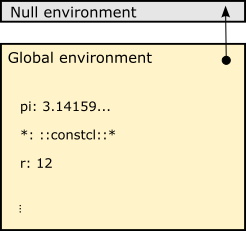
\includegraphics{images/env1.png}


During the call. Note how the global \texttt{r} is shadowed by the local one, and how the local environment links to the global one to find \texttt{*} and \texttt{pi}.


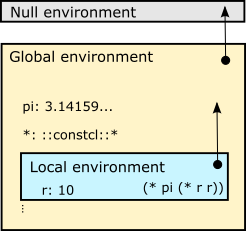
\includegraphics{images/env2.png}


After the call, we are back to the first state again.


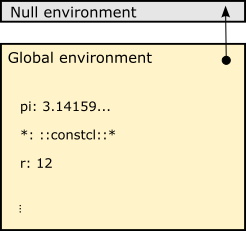
\includegraphics{images/env1.png}

\chapter{Lookup tables}
\label{lookup-tables}

Lisp languages have two simple variants of key/value lookup tables: property lists (plists) and association lists (alists).


A property list is simply a list where every odd-numbered item (starting from 1) is a key and every even-numbered item is a value. Example:

\noindent\makebox[\linewidth]{\rule{\linewidth}{0.4pt}}
\begin{lstlisting}
'(a 1 b 2 c 3 d 4 e 5)
\end{lstlisting}
\noindent\makebox[\linewidth]{\rule{\linewidth}{0.4pt}}

Values can be retrieved in a two-step process:

\noindent\makebox[\linewidth]{\rule{\linewidth}{0.4pt}}
\begin{lstlisting}
> (define plist (list 'a 1 'b 2 'c 3 'd 4 'e 5))
> (define v '())
> (set! v (memq 'c plist))
(c 3 d 4 e 5)
> (set! v (cadr v))
3
\end{lstlisting}
\noindent\makebox[\linewidth]{\rule{\linewidth}{0.4pt}}

If a key doesn't occur in the plist, \texttt{memq} returns \texttt{\#f}.


Alternatively, ConsTcl users can use \texttt{get} to access the value in one step.

\noindent\makebox[\linewidth]{\rule{\linewidth}{0.4pt}}
\begin{lstlisting}
> (get plist 'c)
3
\end{lstlisting}
\noindent\makebox[\linewidth]{\rule{\linewidth}{0.4pt}}

\texttt{get} returns \texttt{\#f} if the key isn't present in the plist.


Values can be added with a single statement:

\noindent\makebox[\linewidth]{\rule{\linewidth}{0.4pt}}
\begin{lstlisting}
> (set! plist (append '(f 6) plist))
(f 6 a 1 b 2 c 3 d 4 e 5)
\end{lstlisting}
\noindent\makebox[\linewidth]{\rule{\linewidth}{0.4pt}}

or with the \texttt{put!} macro, which can both update existing values and add new ones:

\noindent\makebox[\linewidth]{\rule{\linewidth}{0.4pt}}
\begin{lstlisting}
> (put! plist 'c 9)
(f 6 a 1 b 2 c 9 d 4 e 5)
> (put! plist 'g 7)
(g 7 f 6 a 1 b 2 c 9 d 4 e 5)
\end{lstlisting}
\noindent\makebox[\linewidth]{\rule{\linewidth}{0.4pt}}

To get rid of a key/value pair, the simplest way is to add a masking pair:

\noindent\makebox[\linewidth]{\rule{\linewidth}{0.4pt}}
\begin{lstlisting}
> (set! plist (append '(d #f) plist))
(d #f g 7 f 6 a 1 b 2 c 3 d 4 e 5)
\end{lstlisting}
\noindent\makebox[\linewidth]{\rule{\linewidth}{0.4pt}}

But instead, one can use the \texttt{del!} macro:

\noindent\makebox[\linewidth]{\rule{\linewidth}{0.4pt}}
\begin{lstlisting}
> plist
(g 7 f 6 a 1 b 2 c 9 d 4 e 5)
> (del! plist 'd)
(g 7 f 6 a 1 b 2 c 9 e 5)
\end{lstlisting}
\noindent\makebox[\linewidth]{\rule{\linewidth}{0.4pt}}

An alist is a list where the items are pairs, with the key as the \texttt{car} and the value as the \texttt{cdr}. Example:

\noindent\makebox[\linewidth]{\rule{\linewidth}{0.4pt}}
\begin{lstlisting}
> (define alist (list (cons 'a 1) (cons 'b 2) (cons 'c 3) (cons 'd 4)))
> alist
((a . 1) (b . 2) (c . 3) (d . 4))
\end{lstlisting}
\noindent\makebox[\linewidth]{\rule{\linewidth}{0.4pt}}

An alist can also be created from scratch using the \texttt{pairlis} procedure:

\noindent\makebox[\linewidth]{\rule{\linewidth}{0.4pt}}
\begin{lstlisting}
> (define alist (pairlis '(a b c) '(1 2 3)))
((a . 1) (b . 2) (c . 3))
\end{lstlisting}
\noindent\makebox[\linewidth]{\rule{\linewidth}{0.4pt}}

The procedure \texttt{assq} retrieves one pair based on the key:

\noindent\makebox[\linewidth]{\rule{\linewidth}{0.4pt}}
\begin{lstlisting}
> (assq 'a alist)
(a . 1)
> (cdr (assq 'a alist))
1
> (assq 'x alist)
#f
\end{lstlisting}
\noindent\makebox[\linewidth]{\rule{\linewidth}{0.4pt}}

As an alternative, the \texttt{get-alist} procedure fetches the value directly, or \#f for a missing item:

\noindent\makebox[\linewidth]{\rule{\linewidth}{0.4pt}}
\begin{lstlisting}
> (get-alist 'a)
1
> (get-alist 'x)
#f
\end{lstlisting}
\noindent\makebox[\linewidth]{\rule{\linewidth}{0.4pt}}

We can add another item to the alist with the \texttt{push!} macro:

\noindent\makebox[\linewidth]{\rule{\linewidth}{0.4pt}}
\begin{lstlisting}
> (push! (cons 'e 5) alist)
((e . 5) (a . 1) (b . 2) (c . 3) (d . 4))
\end{lstlisting}
\noindent\makebox[\linewidth]{\rule{\linewidth}{0.4pt}}

The \texttt{set-alist!} procedure can be used to update a value (it returns the alist unchanged if the key isn't present):

\noindent\makebox[\linewidth]{\rule{\linewidth}{0.4pt}}
\begin{lstlisting}
> alist
((a . 1) (b . 2) (c . 3) (d . 4))
> (set-alist! alist 'b 7)
((a . 1) (b . 7) (c . 3) (d . 4))
\end{lstlisting}
\noindent\makebox[\linewidth]{\rule{\linewidth}{0.4pt}}
\chapter{A Scheme base}
\label{a-scheme-base}
\noindent\makebox[\linewidth]{\rule{\linewidth}{0.4pt}}
\begin{lstlisting}
 
; An assortment of procedures to supplement the builtins.
 
(define (get plist key)
  (let ((v (memq key plist)))
    (if v
      (cadr v)
      #f)))
 
(define (list-find-key lst key)
 
(define (lfk lst key count)
  (if (null? lst)
    -1
    (if (eq? (car lst) key)
      count
      (lfk (cddr lst) key (+ count 2)))))
 
(define (list-set! lst idx val)
  (if (zero? idx)
    (set-car! lst val)
    (list-set! (cdr lst) (- idx 1) val)))
 
(define (delete! lst key)
  (let ((idx (list-find-key lst key)))
      lst
        (set! lst (cddr lst))
        (let ((bef (del-seek lst (- idx 1)))
              (aft (del-seek lst (+ idx 2))))
          (set-cdr! bef aft))))
    lst))
 
(define (del-seek lst idx)
  (if (zero? idx)
    lst
    (del-seek (cdr lst) (- idx 1))))
 
(define (get-alist lst key)
  (let ((item (assq key lst)))
    (if item
      (cdr item)
      #f)))
 
(define (pairlis a b)
  (if (null? a)
    ()
    (cons
      (cons (car a) (car b))
      (pairlis (cdr a) (cdr b)))))
 
(define (set-alist! lst key val)
  (let ((item (assq key lst)))
    (if item
      (begin (set-cdr! item val) lst)
      lst)))
 
(define (fact n)
  (if (<= n 1)
    1
    (* n (fact (- n 1)))))
 
\end{lstlisting}
\noindent\makebox[\linewidth]{\rule{\linewidth}{0.4pt}}

\end{document}
